% ============================================================
%  Fichier principal : main.tex
%  Mémoire de Master BIBDA — CHOUFA ZOUHAIR
%  Université Chouaib Doukkali — Faculté des Sciences El Jadida
% ============================================================
\documentclass[12pt,a4paper]{report}
\usepackage[utf8]{inputenc}
\usepackage[french]{babel}
\usepackage{graphicx}
\usepackage{tikz}
\usepackage{hyperref}
\usepackage{xcolor}
\usepackage{geometry}
\usepackage{float}
\usepackage{longtable}
\usepackage{makecell}
\usepackage{amssymb}
\usepackage{pgfplots}
\usetikzlibrary{calc}
\pgfplotsset{compat=1.18}
\usepackage[T1]{fontenc}
\usetikzlibrary{positioning, fit, shapes.geometric}

\geometry{top=2.5cm, bottom=2.5cm, left=2.5cm, right=2.5cm}

% --- Couleurs pour la page de garde ---
% \definecolor{lineblue}{RGB}{0, 102, 204}
% \definecolor{bordergreen}{RGB}{0, 153, 76}
% \definecolor{titleblue}{RGB}{0, 51, 102}

\definecolor{lineblue}{RGB}{119,179,224}
\definecolor{titleblue}{RGB}{20,118,186}
\definecolor{bordergreen}{RGB}{128,186,104}

\begin{document}

% ─────────────────────────────────────────────────────────────
%  PAGE DE GARDE (Sans numérotation visible)
% ─────────────────────────────────────────────────────────────
\hypersetup{pageanchor=false}
% --- title.tex ---
\begin{titlepage}
\begin{tikzpicture}[remember picture, overlay]
    \draw[line width=1.5pt] ([shift={(1cm,-1cm)}]current page.north west) rectangle ([shift={(-1cm,1cm)}]current page.south east);
    \draw[line width=0.5pt] ([shift={(1.1cm,-1.1cm)}]current page.north west) rectangle ([shift={(-1.1cm,1.1cm)}]current page.south east);
\end{tikzpicture}

\begin{center}
\noindent
\begin{minipage}[c]{0.2\textwidth}
    
\includegraphics[width=\textwidth]{pics/faculte_logo.jpg}
\end{minipage}%
\begin{minipage}[c]{0.6\textwidth}
    \centering
    \small \textbf{UNIVERSITÉ CHOUAIB DOUKKALI}\\[0.2cm]
    \small \textbf{FACULTÉ DES SCIENCES -- EL JADIDA}\\[0.2cm]
    \small \textbf{DÉPARTEMENT D'INFORMATIQUE}\\[0.2cm]
    \textcolor{lineblue}{\rule{0.8\textwidth}{1.5pt}}
\end{minipage}%
\begin{minipage}[c]{0.2\textwidth}
    \raggedleft
    
\includegraphics[width=\textwidth]{pics/University_logo.jpg}
\end{minipage}

\vspace{1.2cm}
{\Huge \textbf{Mémoire de Master}}\\[1cm]
\textcolor{lineblue}{\rule{0.9\textwidth}{1.5pt}}\\[0.5cm]
{\large \textbf{Pour l’obtention du diplôme de Master en Business Intelligence and Big Data Analytics}}\\[0.5cm]
\textcolor{lineblue}{\rule{0.9\textwidth}{1.5pt}}\\[1.5cm]

{\large \textbf{Sur le sujet de :}}\\[0.8cm]

\begin{tikzpicture}
    \node[
        draw=bordergreen, 
        rounded corners=12pt, 
        inner sep=15pt, 
        text width=0.9\textwidth, 
        align=center,
        font=\LARGE\bfseries,
        text=titleblue 
    ] {
        Gestion de l'hétérogénéité des données tabulaires
        pour la génération de Knowledge Graphs \\ (Big Data + KG)
    };  
\end{tikzpicture}\\[1cm]

{\large \textit{\textbf{Par :}}}\\[0.3cm]
{\large \textbf{CHOUFA Zouhair}}\\[1cm]

Soutenu le : 10-07-2026 , devant le jury composé de :\\[0.8cm]

\begin{tabular}{p{4.5cm} p{6.5cm} p{3cm}}
    \textbf{Pr. A. MADANI} & Faculté des Sciences - El Jadida & Encadrant \\
    \textbf{Pr. } & Faculté des Sciences - El Jadida & Examinateur \\
    \textbf{Pr. } & Faculté des Sciences - El Jadida & Examinateur \\
\end{tabular}
\vspace{1cm}
\vfill
Année universitaire : 2025-2026
\end{center}
\end{titlepage}
\clearpage
% --- NOUVELLE PAGE BLANCHE ---
\thispagestyle{empty} % S'assure qu'aucun numéro n'apparaît
\null                 % Insère une "boîte vide" pour tromper LaTeX
\clearpage
% -----------------------------

% ─────────────────────────────────────────────────────────────
%  ÉLÉMENTS LIMINAIRES — Numérotation Romaine (i, ii, iii...)
% ─────────────────────────────────────────────────────────────
\hypersetup{pageanchor=true}  
\pagestyle{plain}             % <--- NOUVEAU : Force l'affichage visible des numéros en bas de page
\pagenumbering{roman}         

% ============================================================
%  Dédicace — Mémoire de Master BIBDA — CHOUFA Zouhair
% ============================================================
\clearpage

% \thispagestyle{empty}
\begin{tikzpicture}[remember picture, overlay]
    % Cadre décoratif discret aux quatre coins de la page
    \draw[line width=1pt, titleblue]
        ([shift={(1.5cm,-1.5cm)}]current page.north west) -- ++(1.4cm,0);
    \draw[line width=1pt, titleblue]
        ([shift={(1.5cm,-1.5cm)}]current page.north west) -- ++(0,-1.4cm);

    \draw[line width=1pt, titleblue]
        ([shift={(-1.5cm,-1.5cm)}]current page.north east) -- ++(-1.4cm,0);
    \draw[line width=1pt, titleblue]
        ([shift={(-1.5cm,-1.5cm)}]current page.north east) -- ++(0,-1.4cm);

    \draw[line width=1pt, bordergreen]
        ([shift={(1.5cm,1.5cm)}]current page.south west) -- ++(1.4cm,0);
    \draw[line width=1pt, bordergreen]
        ([shift={(1.5cm,1.5cm)}]current page.south west) -- ++(0,1.4cm);

    \draw[line width=1pt, bordergreen]
        ([shift={(-1.5cm,1.5cm)}]current page.south east) -- ++(-1.4cm,0);
    \draw[line width=1pt, bordergreen]
        ([shift={(-1.5cm,1.5cm)}]current page.south east) -- ++(0,1.4cm);

    % Petit motif de noeud sémantique (rappel Knowledge Graph) en filigrane
    \begin{scope}[opacity=0.55, shift={($(current page.center)+(0,-8.5cm)$)}]
        \node[circle, draw=lineblue, fill=lineblue!15, minimum size=5pt, inner sep=0pt] (n1) at (0,0) {};
        \node[circle, draw=titleblue, fill=titleblue!15, minimum size=5pt, inner sep=0pt] (n2) at (0.9,0.35) {};
        \node[circle, draw=bordergreen, fill=bordergreen!15, minimum size=5pt, inner sep=0pt] (n3) at (1.6,-0.25) {};
        \node[circle, draw=lineblue, fill=lineblue!15, minimum size=5pt, inner sep=0pt] (n4) at (-0.9,0.3) {};
        \node[circle, draw=titleblue, fill=titleblue!15, minimum size=5pt, inner sep=0pt] (n5) at (-1.6,-0.2) {};
        \draw[lineblue!70] (n1) -- (n2);
        \draw[titleblue!70] (n2) -- (n3);
        \draw[bordergreen!70] (n1) -- (n3);
        \draw[lineblue!70] (n1) -- (n4);
        \draw[titleblue!70] (n4) -- (n5);
        \draw[bordergreen!70] (n1) -- (n5);
    \end{scope}
\end{tikzpicture}

\vspace*{2.2cm}
\begin{center}
    {\Large \scshape \color{titleblue} \textbf{Dédicace}} \\[0.15cm]
    \textcolor{bordergreen}{\rule{4.5cm}{0.8pt}}
\end{center}

\vspace{1.8cm}

\begin{center}
\begin{minipage}{0.82\textwidth}
\setlength{\parindent}{0pt}
\raggedright
\Large
\itshape

À mes très chers parents, \\[0.3cm]
\normalsize\upshape
dont l'amour inconditionnel, les sacrifices silencieux et la confiance
jamais démentie ont tracé, bien avant moi, le chemin de chacune de mes
réussites. Que ce modeste travail soit le reflet, même imparfait, de
tout ce que je vous dois.

\vspace{0.9cm}
\Large\itshape
À mes frères et sœurs, \\[0.3cm]
\normalsize\upshape
pour votre soutien constant, vos encouragements dans les moments de
doute, et la complicité qui nous unit depuis toujours.

\vspace{0.9cm}
\Large\itshape
À mes amis et collègues de la promotion BIBDA, \\[0.3cm]
\normalsize\upshape
compagnons de cette aventure académique exigeante, avec qui chaque
nuit blanche de débogage et chaque réussite ont pris un sens partagé.

\vspace{0.9cm}
\Large\itshape
À tous ceux qui croient qu'une donnée brute, aussi hétérogène
soit-elle, peut devenir connaissance structurée pour peu qu'on lui
consacre la rigueur et la patience nécessaires, \\[0.3cm]
\normalsize\upshape
ce mémoire vous est dédié.

\end{minipage}
\end{center}

\vfill
\begin{center}
    \textcolor{lineblue}{\rule{6cm}{0.6pt}}\\[0.25cm]
    {\small \itshape ``Les données ne parlent pas d'elles-mêmes ;\\
    c'est la structure qu'on leur donne qui les fait parler.''}
\end{center}
\vspace{1.5cm}

\newpage
% ============================================================
%  Remerciements — Mémoire de Master BIBDA — CHOUFA Zouhair
% ============================================================
\clearpage
\thispagestyle{empty}

\begin{center}
    \vspace*{1cm} 
    {\Huge \scshape \color{titleblue} \textbf{Remerciements}} \\[0.2cm]
    \textcolor{bordergreen}{\rule{1cm}{1.2pt}}
    \vspace{1cm} 
\end{center}
\addcontentsline{toc}{chapter}{Remerciements}
\renewcommand{\baselinestretch}{1.15}\normalsize

Au terme de ce travail, il est adressé une gratitude sincère à toutes
les personnes ayant contribué, directement ou indirectement, à la
réalisation de ce mémoire.

Les remerciements les plus sincères sont exprimés au
\textbf{Professeur A. MADANI}, encadrant de ce travail à la Faculté
des Sciences d'El Jadida, pour la qualité de son encadrement, sa
disponibilité constante et la pertinence de ses conseils tout au long
de ce projet. Sa rigueur scientifique et la confiance accordée dans
la conduite de ce sujet de recherche ont permis de mener cette étude
dans les meilleures conditions.

Les membres du jury sont également remerciés pour l'honneur qu'ils
font en évaluant ce travail. Leur lecture attentive et leurs
remarques constitueront un apport précieux à la poursuite de cette
réflexion scientifique.

Une reconnaissance particulière est adressée au corps professoral et
administratif du \textbf{Département d'Informatique} de la Faculté
des Sciences d'El Jadida, ainsi qu'à \\ l'\textbf{Université Chouaib
Doukkali}, pour la qualité de la formation dispensée durant ce
Master, dont les enseignements théoriques et pratiques ont constitué
le socle de ce travail.

Les camarades de la promotion BIBDA sont remerciés pour l'esprit
d'entraide et les échanges techniques qui ont accompagné ce parcours,
en particulier durant les phases les plus intenses de développement
et de rédaction.

Une pensée est également adressée à la communauté scientifique et
technique open source — notamment les contributeurs des projets
\texttt{Morph-KGC}, \texttt{RDFLib}, \texttt{Splink},
\texttt{Sentence-- Transformers} et \texttt{LangChain} — dont les
outils ont rendu possible l'implémentation du pipeline présenté dans
ce mémoire.

Enfin, les remerciements les plus profonds vont à la famille, pour
son soutien indéfectible, ses encouragements constants et les
sacrifices consentis tout au long de ce parcours académique. Sans ce
soutien, ce mémoire n'aurait pu voir le jour.

\newpage
% ============================================================
%  Résumé (FR) & Abstract (EN) — Mémoire de Master BIBDA
%  CHOUFA Zouhair
% ============================================================

% ─────────────────────────────────────────────────────────────
%  RÉSUMÉ (FRANÇAIS)
% ─────────────────────────────────────────────────────────────
\clearpage
% \thispagestyle{empty}

% Local adjustment to reduce top spacing and center the title
\begin{center}
    \vspace*{-1cm} % Pulls the title up into the empty white space
    {\Huge\bfseries Résumé}
    \vspace{0.5cm} % Space before the paragraph starts
\end{center}
\addcontentsline{toc}{chapter}{Résumé}

La dimension « Variété » du Big Data se traduit, en contexte
industriel, par la coexistence de multiples sources de données
tabulaires hétérogènes (formats, schémas, conventions de nommage),
rendant leur intégration sémantique difficile à automatiser à grande
échelle. Les Knowledge Graphs (KG), fondés sur le modèle RDF et les
standards du Web sémantique, offrent un cadre formel pour unifier ces
sources autour d'une ontologie commune ; toutefois, les pipelines de
construction existants restent le plus souvent fragmentés,
partiellement manuels, ou insuffisamment évalués de bout en bout.

Ce mémoire propose un pipeline complet, modulaire et reproductible de
transformation de données tabulaires hétérogènes en Knowledge Graph.
L'architecture proposée s'articule en quatre modules~: (i) ingestion
multi-source et profilage automatique de la qualité des données ;
(ii) \textit{schema matching} hybride combinant une approche
symbolique par embeddings Sentence-BERT et un agent LLM (LLaMA~3.1
via Groq, orchestré par LangChain), suivi de la génération
automatique de règles de mapping YARRRML ; (iii) triplification
sémantique déclarative des données au moyen du moteur Morph-KGC ;
(iv) résolution d'entités inter-sources par le modèle probabiliste de
Fellegi-Sunter (bibliothèque Splink), complétée par une validation
formelle du graphe produit via des contraintes SHACL. L'ensemble du
pipeline est conteneurisé avec Docker Compose afin de garantir sa
reproductibilité et son industrialisation potentielle.

L'approche a été évaluée sur un gold standard annoté, construit à
partir d'un jeu de données transactionnel augmenté artificiellement
(\texttt{Faker}) et scindé en deux sources hétérogènes simulant des
silos organisationnels distincts. Les résultats montrent que
l'architecture hybride de \textit{schema matching} atteint un
F1-score de 0,870 après calibration du seuil de décision
($\tau^{*} = 0{,}82$), égalant ou surpassant chacune de ses
composantes utilisée isolément tout en maîtrisant le coût des appels
LLM. Le module de triplification génère 82\,420 triplets RDF en
seulement 7 secondes, tandis que la résolution d'entités, évaluée sur
1\,600 paires réelles, atteint un F1-score de 0,990 après recalibrage
des règles de blocage ($\lambda^{*} = 0{,}90$). Une discussion
critique structurée autour des menaces classiques à la validité
expérimentale (interne, externe, de construit et de conclusion)
complète cette évaluation et identifie les limites du travail,
notamment le caractère synthétique du jeu de données et la
sensibilité du modèle de résolution d'entités à la configuration des
règles de blocage.

Ce travail démontre ainsi la faisabilité d'un pipeline hybride
symbolique-neuronal pour la construction automatisée et évaluable de
Knowledge Graphs à partir de données tabulaires hétérogènes, et ouvre
plusieurs perspectives~: validation sur des données réelles
anonymisées, définition automatique de clés de blocage adaptatives,
et substitution des appels LLM distants par des modèles open source
déployés localement afin de réduire la latence à grande échelle.

\vspace{0.8cm}
\noindent\textbf{Mots-clés~:} Big Data, Knowledge Graph, hétérogénéité
des données, \textit{schema matching}, Large Language Models,
RDF, YARRRML, Morph-KGC, résolution d'entités, SHACL, reproductibilité.

\newpage

% ─────────────────────────────────────────────────────────────
%  ABSTRACT (ENGLISH)
% ─────────────────────────────────────────────────────────────
% \thispagestyle{empty}

\begin{center}
    \vspace*{-1cm} % Pulls the Abstract up identically
    {\Huge\bfseries Abstract}
    \vspace{0.5cm}
\end{center}
\addcontentsline{toc}{chapter}{Abstract}

The "Variety" dimension of Big Data manifests, in industrial
settings, as the coexistence of multiple heterogeneous tabular data
sources differing in format, schema, and naming conventions, making
their semantic integration difficult to automate at scale. Knowledge
Graphs (KGs), built upon the RDF model and Semantic Web standards,
provide a formal framework for unifying such sources around a shared
ontology; however, existing construction pipelines remain, for the
most part, fragmented, partially manual, or insufficiently evaluated
end-to-end.

This thesis proposes a complete, modular, and reproducible pipeline
for transforming heterogeneous tabular data into a Knowledge Graph.
The proposed architecture is organized into four modules: (i)
multi-source ingestion and automated data quality profiling; (ii) a
hybrid schema matching approach combining a symbolic
Sentence-BERT embedding method with an LLM agent (LLaMA~3.1 via Groq,
orchestrated through LangChain), followed by the automatic generation
of YARRRML mapping rules; (iii) declarative semantic triplification
of the data using the Morph-KGC engine; (iv) cross-source entity
resolution based on the Fellegi-Sunter probabilistic model (Splink
library), complemented by a formal validation of the resulting graph
through SHACL constraints. The entire pipeline is containerized with
Docker Compose to ensure reproducibility and potential
industrialization.

The approach was evaluated on an annotated gold standard, built from
a transactional dataset artificially augmented via \texttt{Faker} and
split into two heterogeneous sources simulating distinct
organizational silos. Results show that the hybrid schema matching
architecture achieves an F1-score of 0.870 after calibrating the
decision threshold ($\tau^{*} = 0.82$), matching or outperforming
each of its components used in isolation while keeping LLM API costs
under control. The triplification module generates 82,420 RDF
triples in only 7 seconds, while entity resolution, evaluated on
1,600 real pairs, reaches an F1-score of 0.990 after recalibrating
the blocking rules ($\lambda^{*} = 0.90$). A critical discussion
structured around the classical threats to experimental validity
(internal, external, construct, and conclusion validity) complements
this evaluation and identifies the work's limitations, notably the
synthetic nature of the dataset and the sensitivity of the entity
resolution model to blocking rule configuration.

This work thus demonstrates the feasibility of a hybrid
symbolic-neural pipeline for the automated and evaluable construction
of Knowledge Graphs from heterogeneous tabular data, and opens
several avenues for future work: validation on real anonymized data,
automatic definition of adaptive blocking keys, and the substitution
of remote LLM calls with locally deployed open-source models to
reduce latency at scale.

\vspace{0.8cm}
\noindent\textbf{Keywords:} Big Data, Knowledge Graph, data
heterogeneity, schema matching, Large Language Models, RDF, YARRRML,
Morph-KGC, entity resolution, SHACL, reproducibility.

\newpage

% ─────────────────────────────────────────────────────────────
%  TABLES ET LISTES
% ─────────────────────────────────────────────────────────────
\tableofcontents
\newpage
\input{gen/figures.tex}
\newpage
\input{gen/tables.tex}
\newpage
% ============================================================
%  Liste des Abréviations — Mémoire de Master BIBDA
%  CHOUFA Zouhair
%  NOTE : nécessite \usepackage{longtable} dans le préambule
%         de main.tex (voir instructions fournies).
% ============================================================
\chapter*{Liste des Abréviations}
\addcontentsline{toc}{chapter}{Liste des Abréviations}

\begin{longtable}{p{3.2cm} p{10.8cm}}
\hline
\textbf{Abréviation} & \textbf{Signification} \\
\hline
\endfirsthead
\multicolumn{2}{l}{\textit{(suite de la page précédente)}} \\
\hline
\textbf{Abréviation} & \textbf{Signification} \\
\hline
\endhead
\hline
\multicolumn{2}{r}{\textit{(suite sur la page suivante)}} \\
\endfoot
\hline
\endlastfoot

API       & Application Programming Interface (interface de programmation applicative) \\
BD        & Big Data \\
BIBDA     & Business Intelligence and Big Data Analytics (intitulé du Master) \\
CLI       & Command Line Interface (interface en ligne de commande) \\
CRM       & Customer Relationship Management (gestion de la relation client) \\
CSV       & Comma-Separated Values (valeurs séparées par des virgules) \\
DL        & Deep Learning (apprentissage profond) \\
EM        & Expectation-Maximization (algorithme espérance-maximisation) \\
FOAF      & Friend Of A Friend (vocabulaire RDF de description de réseaux sociaux) \\
GPT       & Generative Pre-trained Transformer \\
GraphDB   & Triplestore RDF développé par Ontotext, utilisé pour le stockage du KG produit \\
IA        & Intelligence Artificielle \\
ISO       & International Organization for Standardization (organisation internationale de normalisation) \\
JSON      & JavaScript Object Notation (format d'échange de données) \\
KG        & Knowledge Graph (graphe de connaissances) \\
KGs       & Knowledge Graphs (pluriel) \\
LangChain & Framework open source d'orchestration d'agents et de \textit{prompts} pour LLMs \\
LLaMA     & Large Language Model Meta AI (famille de modèles de langage de Meta) \\
LLM       & Large Language Model (grand modèle de langage) \\
LLMs      & Large Language Models (pluriel) \\
LLMatch   & Méthode de \textit{schema matching} fondée sur les LLMs (littérature) \\
Morph-KGC & Moteur de triplification déclarative RML/YARRRML utilisé au Module~3 du pipeline \\
NLP       & Natural Language Processing (traitement automatique du langage naturel) \\
OAEI      & Ontology Alignment Evaluation Initiative (initiative d'évaluation de l'alignement d'ontologies) \\
OWL       & Web Ontology Language (langage d'ontologies du Web sémantique) \\
PySHACL   & Bibliothèque Python d'implémentation du langage de contraintes SHACL \\
PyVis     & Bibliothèque Python de visualisation interactive de graphes \\
R2RML     & RDB to RDF Mapping Language (standard W3C de mapping base relationnelle vers RDF) \\
RDB       & Relational DataBase (base de données relationnelle) \\
RDF       & Resource Description Framework (modèle de données du Web sémantique) \\
RDFLib    & Bibliothèque Python de manipulation de graphes RDF \\
REST      & Representational State Transfer (style d'architecture d'API Web) \\
RML       & RDF Mapping Language (standard W3C de mapping générique vers RDF) \\
SBERT     & Sentence-BERT (modèle d'embeddings de phrases fondé sur BERT) \\
SCHEMORA  & Méthode d'alignement de schémas par \textit{prompt engineering} (littérature) \\
SemTab    & Semantic Table Interpretation Challenge (banc d'essai communautaire d'interprétation sémantique de tables) \\
SHACL     & Shapes Constraint Language (langage W3C de validation de graphes RDF) \\
SIRH      & Système d'Information des Ressources Humaines \\
SPARQL    & SPARQL Protocol And RDF Query Language (langage de requête pour RDF) \\
SQL       & Structured Query Language (langage de requête structuré) \\
SQLite    & Système de gestion de base de données relationnelle embarqué \\
STI       & Semantic Table Interpretation (interprétation sémantique de tables) \\
TF-IDF    & Term Frequency--Inverse Document Frequency (pondération statistique de termes) \\
URI       & Uniform Resource Identifier (identifiant uniforme de ressource) \\
URIs      & Uniform Resource Identifiers (pluriel) \\
UTF-8     & Unicode Transformation Format -- 8 bits (encodage de caractères) \\
W3C       & World Wide Web Consortium (organisme de standardisation du Web) \\
XML       & eXtensible Markup Language (langage de balisage extensible) \\
XSD       & XML Schema Definition (langage de définition de schémas XML) \\
YAML      & YAML Ain't Markup Language (format de sérialisation de données lisible) \\
YARRRML   & Yet Another RML Rule ML (langage déclaratif simplifié pour la génération de règles RML) \\
$\tau$    & Seuil de décision du Module~2 (schema matching hybride) \\
$\lambda$ & Seuil de décision du Module~4 (résolution d'entités, modèle de Fellegi-Sunter) \\

\end{longtable}

\newpage
\clearpage                    

% ─────────────────────────────────────────────────────────────
%  CORPS DU MÉMOIRE — Numérotation Arabe (1, 2, 3...)
% ─────────────────────────────────────────────────────────────
\pagenumbering{arabic}        % Bascule en 1, 2, 3... (L'affichage reste visible grâce au \pagestyle{plain} précédent)

% ============================================================
%  Introduction Générale — Mémoire de Master BIBDA
%  CHOUFA Zouhair
% ============================================================
\chapter*{Introduction Générale}
\addcontentsline{toc}{chapter}{Introduction Générale}
\label{chap:introduction_generale}
 
\section*{Contexte général}
\addcontentsline{toc}{section}{Contexte général}
 
L'ère du Big Data a profondément transformé la manière dont les
organisations produisent, stockent et exploitent leurs données.
Parmi les cinq dimensions classiquement associées à ce paradigme —
Volume, Vélocité, Variété, Véracité et Valeur —, la \textbf{Variété}
constitue sans doute le défi le plus structurel pour les entreprises
modernes. Une organisation typique dispose rarement d'une source de
données unique et homogène~: ses informations sont dispersées entre
systèmes CRM, bases de données transactionnelles, fichiers plats
CSV, systèmes d'information des ressources humaines (SIRH) ou
tableurs, chacun obéissant à des conventions de nommage, des schémas
et des formats qui lui sont propres. Cette fragmentation, souvent
qualifiée de phénomène des \textit{silos de données}, constitue un
frein majeur à toute exploitation analytique transversale et
cohérente de l'information disponible.
 
Les \textbf{Knowledge Graphs} (KG), fondés sur le modèle de données
RDF (\textit{Resource Description Framework}) et sur les standards du
Web sémantique — OWL, SPARQL, SHACL —, se sont imposés au cours de la
dernière décennie comme un cadre formel particulièrement adapté pour
répondre à ce défi d'intégration. En représentant les entités et
leurs relations sous forme de triplets sujet-prédicat-objet ancrés
dans une ontologie de domaine partagée, les KG permettent de dépasser
la rigidité du modèle relationnel classique et d'unifier
sémantiquement des sources hétérogènes autour d'un vocabulaire
commun. Cette approche a démontré sa valeur dans des contextes aussi
variés que les moteurs de recherche, les systèmes de recommandation,
la biomédecine ou l'intégration de données d'entreprise.
 
\section*{Problématique}
\addcontentsline{toc}{section}{Problématique}
 
Si la valeur des Knowledge Graphs pour l'intégration de données
n'est plus à démontrer, leur \textbf{construction automatisée} à
partir de sources tabulaires hétérogènes demeure un problème ouvert
et largement non résolu de façon industrialisable. La littérature
existante propose des solutions ponctuelles pour chacune des étapes
du processus — schema matching, triplification déclarative via les
standards R2RML/RML, résolution d'entités, validation de la
qualité du graphe produit — mais rarement de manière intégrée au
sein d'un pipeline unique, reproductible et évaluable de bout en
bout. De plus, l'émergence récente des grands modèles de langage
(\textit{Large Language Models}, LLM) ouvre des perspectives
prometteuses pour automatiser des tâches historiquement coûteuses en
intervention humaine, telles que l'alignement sémantique de schémas
hétérogènes, mais leur intégration dans des architectures de
production robustes, maîtrisées en coût et rigoureusement évaluées,
reste largement à explorer.
 
Ce mémoire s'inscrit directement dans ce contexte et cherche à
répondre à la question de recherche suivante~: \textit{comment
concevoir un pipeline automatisé, modulaire et reproductible, capable
de transformer des données tabulaires hétérogènes et multi-sources en
un Knowledge Graph unifié, tout en garantissant la qualité et la
validité formelle du graphe produit à chaque étape du processus~?}
 
\section*{Objectifs du mémoire}
\addcontentsline{toc}{section}{Objectifs du mémoire}
 
Pour répondre à cette problématique, ce travail poursuit quatre
objectifs principaux~:
 
\begin{itemize}
    \item \textbf{Concevoir} une architecture de pipeline modulaire
    couvrant l'ensemble de la chaîne de transformation~: ingestion et
    profilage qualité des sources, alignement sémantique des schémas,
    triplification RDF déclarative et résolution d'entités
    inter-sources ;
    \item \textbf{Combiner} de manière hybride des approches
    symboliques (embeddings Sentence-BERT) et neuronales fondées sur
    les LLM (agent LangChain) pour le \textit{schema matching}, en
    visant à maximiser la qualité d'alignement tout en maîtrisant le
    coût computationnel des appels aux modèles de langage ;
    \item \textbf{Automatiser} la génération des règles de mapping
    YARRRML et leur exécution via le moteur Morph-KGC, ainsi que la
    validation formelle du graphe de connaissances produit au moyen
    de contraintes SHACL ;
    \item \textbf{Évaluer} quantitativement chaque module du pipeline
    sur un gold standard annoté, et discuter de manière critique la
    validité, les limites et la généralisabilité des résultats
    obtenus.
\end{itemize}
 
\section*{Contributions}
\addcontentsline{toc}{section}{Contributions}
 
La contribution de ce mémoire se situe à l'intersection de trois
axes de recherche généralement traités séparément dans la
littérature~: la triplification déclarative de données (RML/YARRRML),
le \textit{schema matching} hybride, et l'automatisation par LLM.
Le pipeline proposé intègre ces trois dimensions au sein d'une
architecture unique, entièrement conteneurisée via Docker Compose,
et dont chaque module fait l'objet d'une évaluation quantitative
indépendante sur un gold standard construit spécifiquement pour ce
travail. Cette approche intégrée et évaluable de bout en bout
constitue, à notre connaissance, une réponse originale aux lacunes
identifiées dans l'état de l'art~: fragmentation des pipelines
existants, absence d'évaluation standardisée, reproductibilité
insuffisante et déficit d'études portant sur la scalabilité.
 
\section*{Organisation du mémoire}
\addcontentsline{toc}{section}{Organisation du mémoire}
 
Ce mémoire est structuré en quatre chapitres. Le
\textbf{Chapitre~1} dresse un état de l'art structuré autour du
paradigme Big Data, des fondements des Knowledge Graphs, des
approches de transformation tabulaire vers RDF et de
\textit{schema matching}, ainsi que de l'apport récent des LLM à ces
problématiques ; il se conclut par le positionnement précis de notre
contribution par rapport aux travaux existants. Le
\textbf{Chapitre~2} présente la méthodologie et la conception
détaillée de l'architecture du pipeline proposé, module par module,
ainsi que le protocole d'évaluation et la constitution du gold
standard. Le \textbf{Chapitre~3} décrit l'implémentation concrète de
ce pipeline dans un environnement Cloud réel, les résultats obtenus
pour chaque module, ainsi qu'une étude d'ablation isolant la
contribution propre de chaque composant du module de
\textit{schema matching}. Enfin, le \textbf{Chapitre~4} propose une
évaluation approfondie et comparative des résultats~: calibration
des hyperparamètres critiques du pipeline, positionnement par rapport
à l'état de l'art, et discussion critique structurée autour des
menaces classiques à la validité expérimentale. Une conclusion
générale synthétise les apports de ce travail, en discute les limites
et propose des perspectives de recherche future.
 
% ============================================================
%  CHAPITRE 1 — État de l'art
%  Mémoire de Master BIBDA — CHOUFA ZOUHAIR
%  Université Chouaib Doukkali — Faculté des Sciences El Jadida
%  Titre : Gestion de l'hétérogénéité des données tabulaires
%           pour la génération de Knowledge Graphs (Big Data + KG)
% ============================================================

\chapter{État de l'art}\label{chap:etat_art}

% ─────────────────────────────────────────────────────────────
\section{Introduction}\label{sec:intro_etat_art}
% ─────────────────────────────────────────────────────────────
Dans l'écosystème numérique contemporain, les organisations produisent et accumulent des données issues de sources toujours plus nombreuses et hétérogènes : fichiers tabulaires (\texttt{CSV}, \texttt{Excel}), bases de données relationnelles, flux JSON/XML, entrepôts analytiques, etc. L'intégration cohérente de ces sources constitue l'un des défis les plus critiques de l'ingénierie des données moderne, car elle conditionne directement la qualité des analyses et des décisions qui en découlent.

Face à cette complexité, les \textit{Knowledge Graphs} (KGs) s'imposent comme une infrastructure sémantique particulièrement adaptée : en modélisant les données non plus comme des valeurs isolées dans des tables, mais comme un réseau d'entités reliées par des relations nommées, ils permettent une interopérabilité et un raisonnement automatique difficiles à atteindre par les approches relationnelles classiques. La transformation automatique de données tabulaires hétérogènes vers cette représentation sémantique soulève cependant des questions scientifiques encore largement ouvertes, notamment autour du \textit{schema matching}, de la triplification déclarative, et du rôle croissant des Large Language Models (LLMs) dans ces pipelines.

Ce chapitre dresse un panorama structuré et critique des travaux existants dans ce domaine. Nous commençons par situer la problématique dans le contexte du Big Data (section~\ref{sec:bigdata}), avant d'introduire les fondements des Knowledge Graphs (section~\ref{sec:intro_kg}). Nous analysons ensuite les approches de construction automatique et d'intégration de données hétérogènes (section~\ref{sec:construction_auto}), la transformation tabulaire vers RDF (section~\ref{sec:tabulaire_rdf}), le schema matching et l'alignement d'ontologies (section~\ref{sec:schema_matching}), et l'apport des LLMs (section~\ref{sec:llms}). Nous concluons par une synthèse des limites identifiées (section~\ref{sec:defis}) et un positionnement précis de notre contribution (section~\ref{sec:positionnement}).

% ─────────────────────────────────────────────────────────────
\section{Le Paradigme Big Data et les Défis de l'Intégration}\label{sec:bigdata}
% ─────────────────────────────────────────────────────────────
\subsection{Les dimensions du Big Data}
Le concept de Big Data est traditionnellement caractérisé par le modèle des « 4V », initialement introduit pour décrire les propriétés fondamentales des données à grande échelle : le \textbf{Volume} (la quantité de données produites, désormais mesurée en pétaoctets dans les grandes organisations), la \textbf{Vélocité} (la vitesse à laquelle les données sont générées et doivent être traitées), la \textbf{Véracité} (la fiabilité et la qualité des données collectées) et, surtout dans le cadre du présent travail, la \textbf{Variété}.

% \begin{figure}[ht]
%     \centering
%     % ── Description visuelle ──────────────────────────────────────────────────
%     % Schéma en quatre quadrants : chaque quadrant représente un « V » avec
%     % une icône représentative (disque pour Volume, chronomètre pour Vélocité,
%     % bouclier pour Véracité, arbre de sources pour Variété).
%     % Le quadrant « Variété » est mis en évidence par un contour coloré plus épais
%     % car c'est la dimension centrale du présent travail.
%     % ─────────────────────────────────────────────────────────────────────────
%     %
%     % Code Mermaid correspondant (commentaire LaTeX) :
%     % graph TD
%     %   V1[Volume\nPétaoctets de données] --> BD((Big Data))
%     %   V2[Vélocité\nFlux en temps réel] --> BD
%     %   V3[Véracité\nQualité et fiabilité] --> BD
%     %   V4[Variété\nCSV · JSON · XML · RDB] --> BD
%     %   style V4 fill:#f0ad4e,stroke:#e08a00,color:#000
%     %
%     \fbox{\parbox{0.85\textwidth}{\centering\vspace{1.2cm}
%     \textit{[Figure : Les 4V du Big Data — insérer ici le diagramme quadrants.]}\\
%     \vspace{1.2cm}}}
%     \caption{Les quatre dimensions du Big Data et la place centrale de la Variété dans la problématique d'intégration.}
%     \label{fig:4v_bigdata}
% \end{figure}

\begin{figure}[ht]
    \centering
    \begin{tikzpicture}[
        node distance=3.5cm,
        % Style pour les 3 V classiques
        standardV/.style={
            draw=gray!80, 
            line width=1pt, 
            rounded corners=8pt, 
            minimum width=4cm, 
            minimum height=2cm, 
            align=center, 
            fill=gray!5,
            font=\small
        },
        % Style mis en évidence pour la Variété (votre sujet)
        highlightV/.style={
            draw=bordergreen, 
            line width=2pt, 
            rounded corners=8pt, 
            minimum width=4.2cm, 
            minimum height=2.2cm, 
            align=center, 
            fill=bordergreen!10,
            font=\small
        },
        % Style pour le centre
        centerNode/.style={
            circle, 
            draw=titleblue, 
            line width=1.5pt, 
            minimum size=3cm, 
            align=center, 
            fill=titleblue!10, 
            font=\large\bfseries\color{titleblue}
        }
    ]

    % Nœud Central
    \node[centerNode] (BD) {Big Data};

    % Les 4 Nœuds (Quadrants)
    \node[standardV] (V1) [above left of=BD, xshift=-2cm, yshift=1.5cm] {
        \textbf{\large Volume}\\[0.1cm]
        Pétaoctets de données\\
        Stockage massif
    };
    
    \node[standardV] (V2) [above right of=BD, xshift=2cm, yshift=1.5cm] {
        \textbf{\large Vélocité}\\[0.1cm]
        Flux en temps réel\\
        Traitement rapide
    };
    
    \node[standardV] (V3) [below left of=BD, xshift=-2cm, yshift=-1.5cm] {
        \textbf{\large Véracité}\\[0.1cm]
        Qualité, fiabilité\\
        Nettoyage des données
    };
    
    \node[highlightV] (V4) [below right of=BD, xshift=2cm, yshift=-1.5cm] {
        \textcolor{bordergreen}{\textbf{\large Variété}}\\[0.1cm]
        \textbf{CSV, JSON, SQL, RDF}\\
        \textbf{Hétérogénéité structurelle}\\
        \textbf{et sémantique}
    };

    % Flèches pointant vers le centre
    \draw[-latex, thick, gray!80] (V1) -- (BD);
    \draw[-latex, thick, gray!80] (V2) -- (BD);
    \draw[-latex, thick, gray!80] (V3) -- (BD);
    
    % Flèche plus épaisse et verte pour la Variété
    \draw[-latex, line width=2pt, bordergreen] (V4) -- (BD);

    \end{tikzpicture}
    
    \vspace{0.5cm}
    \caption{Les quatre dimensions du Big Data et la place centrale de la Variété dans la problématique d'intégration.}
    \label{fig:4v_bigdata}
\end{figure}

\subsection{La Variété : source directe de l'hétérogénéité}
Parmi ces quatre dimensions, la Variété est celle qui génère le plus directement les défis traités dans ce mémoire. Dans un environnement industriel réel, une même entité métier — un client, un produit, une transaction — peut être représentée simultanément dans une feuille de calcul Excel (avec une colonne nommée \texttt{ID\_Client}), dans une base de données relationnelle (avec un attribut \texttt{customer\_id}), et dans un fichier JSON d'export tiers (avec une clé \texttt{buyer}). Ces trois représentations réfèrent au même concept, mais aucun mécanisme automatique standard ne permet de les réconcilier sans intervention humaine ou sans infrastructure sémantique dédiée.

\subsection{Scalabilité et besoins architecturaux}
Dans un contexte Big Data, la scalabilité des processus de transformation est cruciale : un pipeline qui fonctionne correctement sur quelques milliers de lignes doit rester opérationnel sur des millions d'enregistrements provenant de dizaines de sources simultanées. La littérature consultée indique que les approches manuelles ou semi-automatiques d'intégration atteignent rapidement leurs limites dans ces scénarios, justifiant le recours à des pipelines automatisés, déclaratifs et évaluables quantitativement~\cite{wu2023comprehensive, yan2023enterprise}.

% ─────────────────────────────────────────────────────────────
\section{Introduction aux Knowledge Graphs}\label{sec:intro_kg}
% ─────────────────────────────────────────────────────────────
\subsection{Définition et fondements}
Avant d'aborder les techniques spécialisées, il est utile de comprendre intuitivement ce qui distingue un Knowledge Graph d'une base de données classique. Dans une base relationnelle, les données sont organisées en tables dont les colonnes définissent des attributs. La \textit{sémantique} — c'est-à-dire le sens des données — reste implicite, dans la tête du développeur ou enfouie dans des commentaires de code. Un Knowledge Graph, au contraire, \textit{externalise} ce sens : chaque entité, chaque relation et chaque attribut reçoit un identifiant universel dont la définition est consultable et exploitable par une machine.

Hogan et al.~\cite{hogan2021knowledge} proposent la définition de référence dans la littérature : un KG est un graphe orienté dans lequel les nœuds représentent des entités du monde réel et les arêtes des relations nommées entre ces entités, le tout formalisé selon les standards du Web Sémantique.

\subsection{Le modèle RDF et le rôle des URIs}

Le modèle de données fondamental des KGs est le triplet RDF
(\textit{Sujet, Prédicat, Objet}).
Chaque ressource est identifiée par une URI
(Uniform Resource Identifier) universelle.

\paragraph{Exemple concret d'unification sémantique.}
Considérons deux fichiers sources provenant de systèmes distincts.
Le premier contient une colonne \texttt{ID\_Client} ; le second,
une colonne \texttt{Acheteur\_Num}. Dans un schéma relationnel,
ces deux colonnes sont invisibles l'une à l'autre, chacune enfermée
dans son silo applicatif. Dans un KG, elles sont toutes deux mappées
vers la même URI ontologique :
\begin{center}
\texttt{<http://example.org/ontology\#Customer>}
\end{center}
Ce mécanisme d'identification universelle est précisément ce qui
permet de surmonter l'hétérogénéité sémantique entre sources \cite{hogan2021knowledge}.

\paragraph{Anatomie d'un triplet RDF.}
Concrètement, chaque cellule d'un tableau source devient
un \textbf{triplet RDF} de la forme (Sujet, Prédicat, Objet).
Par exemple, la ligne \textit{ID\_Client = 42, Nom = Dupont,
Email = dupont@mail.com} produit les trois triplets suivants :

\begin{itemize}
    \item \texttt{<Customer/42>} \quad
          \texttt{rdf:type} \quad
          \texttt{<ontology\#Customer>}
    \item \texttt{<Customer/42>} \quad
          \texttt{<ontology\#hasName>} \quad
          \texttt{"Dupont"\^{}\^{}xsd:string}
    \item \texttt{<Customer/42>} \quad
          \texttt{<ontology\#hasEmail>} \quad
          \texttt{"dupont@mail.com"\^{}\^{}xsd:string}
\end{itemize}

Le \textbf{Sujet} (\texttt{<Customer/42>}) est l'entité décrite,
identifiée par une URI unique et stable.
Le \textbf{Prédicat} (\texttt{<ontology\#hasName>}) est la propriété
qui relie le sujet à sa valeur ; il est lui-même défini par une URI
pointant vers l'ontologie du domaine.
L'\textbf{Objet} peut être soit une autre URI (pour relier deux entités),
soit un \textit{littéral} typé (une valeur concrète avec son type XSD :
\texttt{xsd:string}, \texttt{xsd:date}, \texttt{xsd:decimal}, etc.).
C'est précisément grâce à ce typage explicite que les hétérogénéités
syntaxiques --- formats de dates, encodages de nombres, séparateurs
décimaux --- sont résolues lors de la transformation.

\paragraph{Graphes nommés et traçabilité de la provenance.}
Une extension importante du modèle RDF est le \textbf{quadruplet}
(Sujet, Prédicat, Objet, Graphe), qui ajoute un quatrième composant
identifiant le \textit{graphe nommé} auquel appartient le triplet.
Dans un pipeline multi-sources, cette extension permet de tracer
l'origine de chaque triplet : un triplet provenant du fichier CRM
et un triplet provenant de l'export RH sont stockés dans deux graphes
nommés distincts, ce qui facilite l'audit de qualité et
la résolution des conflits sémantiques.

% \begin{figure}[ht]
%     \centering
%     % ── Description visuelle ──────────────────────────────────────────────────
%     % Schéma en deux parties (gauche / droite) :
%     %   Gauche : deux tables SQL (TABLE_A avec ID_Client, TABLE_B avec Acheteur_Num)
%     %            reliées par une clé étrangère classique.
%     %   Droite : un graphe RDF avec deux nœuds sources pointant tous deux vers
%     %            le nœud URI <Customer>, lequel est relié à d'autres entités
%     %            (<Order>, <Product>) par des arêtes étiquetées.
%     % Une flèche horizontale centrale symbolise la « transformation sémantique ».
%     % ─────────────────────────────────────────────────────────────────────────
%     %
%     % Code Mermaid correspondant :
%     % graph LR
%     %   subgraph SQL ["Schéma relationnel"]
%     %     TA["TABLE_A\nID_Client"] -- FK --> TB["TABLE_B\nAcheteur_Num"]
%     %   end
%     %   subgraph KG ["Knowledge Graph RDF"]
%     %     CU(<http://ex.org#Customer>) -- placeOrder --> OR(<http://ex.org#Order>)
%     %     CU -- buys --> PR(<http://ex.org#Product>)
%     %   end
%     %   SQL -- "Transformation\nsémantique" --> KG
%     %
%     \fbox{\parbox{0.85\textwidth}{\centering\vspace{1.2cm}
%     \textit{[Figure : Du schéma relationnel au graphe sémantique — insérer ici le diagramme.]}\\
%     \vspace{1.2cm}}}
%     \caption{Passage d'un schéma relationnel fragmenté vers un Knowledge Graph unifié par des URIs communes : illustration du principe d'unification sémantique.}
%     \label{fig:sql_to_kg}
% \end{figure}

\begin{figure}[ht]
    \centering
    \begin{tikzpicture}[>=latex, scale=0.9, transform shape]
        
        % Définition des styles
        \tikzset{
            table/.style={draw=gray!80, thick, rounded corners, fill=gray!5, align=center, minimum width=3.2cm, minimum height=1.5cm},
            uri/.style={draw=titleblue, very thick, circle, fill=titleblue!5, align=center, text width=2.5cm, minimum size=3cm, font=\small},
            concept/.style={draw=titleblue, thick, rounded corners, fill=titleblue!5, align=center, minimum width=2.5cm, minimum height=1cm, font=\small},
            mapping/.style={->, dashed, very thick, bordergreen},
            relation/.style={->, very thick, titleblue}
        }

        % --- PARTIE GAUCHE : Schéma Relationnel ---
        \node[table] (t1) at (0, 2) {\textbf{Table Marketing}\\[0.1cm] \texttt{ID\_Client}};
        \node[table] (t2) at (0, -2) {\textbf{Table Facturation}\\[0.1cm] \texttt{Acheteur\_Num}};

        % Cadre gris pour les silos
        \draw[thick, gray, dashed, rounded corners] (-2.2, -3.5) rectangle (2.2, 3.5);
        \node[gray, font=\bfseries] at (0, 3.1) {Silos Relationnels (Isolés)};

        % --- PARTIE DROITE : Knowledge Graph ---
        \node[uri] (customer) at (6.5, 0) {\textbf{URI Unique}\\[0.1cm] \texttt{<Customer>}};
        \node[concept] (order) at (10.5, 2) {\texttt{<Order>}};
        \node[concept] (product) at (10.5, -2) {\texttt{<Product>}};

        % Cadre bleu pour le KG
        \draw[thick, titleblue, dashed, rounded corners] (4.5, -3.5) rectangle (12.5, 3.5);
        \node[titleblue, font=\bfseries] at (8.5, 3.1) {Knowledge Graph Unifié (RDF)};

        % Relations au sein du KG (arêtes bleues)
        \draw[relation] (customer) -- node[above, sloped, font=\scriptsize\ttfamily] {placeOrder} (order);
        \draw[relation] (customer) -- node[below, sloped, font=\scriptsize\ttfamily] {buys} (product);

        % --- CENTRE : Mapping Sémantique (Les flèches vertes) ---
        \draw[mapping] (t1.east) -- node[above, sloped, text=bordergreen, font=\footnotesize\bfseries] {Unification} (customer.150);
        \draw[mapping] (t2.east) -- node[below, sloped, text=bordergreen, font=\footnotesize\bfseries] {Unification} (customer.210);

    \end{tikzpicture}
    
    \vspace{0.5cm}
    \caption{Passage d'un schéma relationnel fragmenté vers un Knowledge Graph unifié par des URIs communes : illustration du principe d'unification sémantique.}
    \label{fig:sql_to_kg}
\end{figure}

\subsection{Les composants du Web Sémantique}
Au-delà du modèle RDF, l'écosystème du Web Sémantique propose une pile technologique complémentaire :
\begin{itemize}
    \item \textbf{RDFS} (\textit{RDF Schema}) permet de définir des hiérarchies de classes et de propriétés, ajoutant une première couche d'inférence.
    \item \textbf{OWL} (\textit{Web Ontology Language}) fournit un langage expressif pour modéliser des contraintes logiques complexes et permettre un raisonnement automatique par inférence. Par exemple, une règle OWL peut déduire automatiquement que deux entités de sources différentes représentent le même individu réel.
    \item \textbf{SPARQL} est le langage de requête standardisé pour interroger les graphes RDF de manière expressive, analogue au SQL pour les bases relationnelles.
    \item \textbf{SHACL} (\textit{Shapes Constraint Language}) permet de définir et de vérifier des contraintes de validation sur la structure d'un graphe RDF, garantissant la conformité du graphe produit à l'ontologie cible.
\end{itemize}
Ce cadre formel constitue le fondement théorique du pipeline de transformation que nous proposons dans ce travail.

% ─────────────────────────────────────────────────────────────
\section{Construction Automatique et Intégration de Données Hétérogènes}\label{sec:construction_auto}
% ─────────────────────────────────────────────────────────────
\subsection{Formalisation du problème}
La construction automatique de KGs à partir de sources hétérogènes est un défi central du domaine. Wu et al.~\cite{wu2023comprehensive} le formalisent à travers le théorème HACE (\textit{Heterogeneous, Autonomous, Complex, Evolving}), qui caractérise les quatre dimensions problématiques des environnements Big Data. Leur survey de référence, publié dans \textit{ACM Computing Surveys}, recense les méthodes d'extraction d'entités nommées (NER), d'extraction de relations et de fusion de connaissances, et souligne que chaque étape du pipeline introduit des erreurs cumulatives susceptibles de dégrader la qualité du graphe final. Cette observation sur l'\textit{accumulation d'erreurs} constitue l'une des motivations majeures pour développer des pipelines intégrés plutôt que séquentiels.

\subsection{Pipelines d'entreprise}
Dans un contexte industriel, Yan et al.~\cite{yan2023enterprise} proposent un cadre de processus complet pour la construction d'un KG combinant données structurées et non structurées. Leur pipeline couvre l'acquisition, le prétraitement, l'extraction d'information, la fusion et la mise à jour du KG. Les auteurs démontrent que la qualité du KG produit est directement liée à la rigueur du traitement de l'hétérogénéité en amont. Cette approche constitue un point de comparaison direct pour notre travail, bien qu'elle demeure partiellement manuelle dans sa phase d'alignement de schémas — limitation que notre approche vise précisément à dépasser.

Il convient de souligner une limitation méthodologique récurrente dans ce type de travaux : les pipelines proposés sont souvent décrits à un niveau d'abstraction élevé, sans environnement d'exécution normalisé ni mécanisme de validation formelle du graphe produit, ce qui nuit considérablement à leur reproductibilité~\cite{wu2023comprehensive}.

\subsection{Taxonomie de l'hétérogénéité}
La littérature consultée converge vers une taxonomie tripartite bien documentée des formes d'hétérogénéité~\cite{survey_heterogeneous_kg_2023} :
\begin{enumerate}
    \item \textbf{Hétérogénéité structurelle} : différences dans l'organisation des données entre sources (tables normalisées vs. fichiers plats, hiérarchies JSON vs. schémas relationnels).
    \item \textbf{Hétérogénéité syntaxique} : mêmes valeurs encodées différemment selon les systèmes (formats de dates, encodages de caractères, unités de mesure).
    \item \textbf{Hétérogénéité sémantique} : mêmes concepts désignés par des termes différents selon les domaines ou les organisations (\texttt{ID\_Client} vs. \texttt{Acheteur\_Num} vs. \texttt{buyer\_id}).
\end{enumerate}
Cette classification est désormais le cadre de référence standard pour décrire les défis d'intégration dans les pipelines de transformation vers KG, et structure directement l'architecture en couches que nous proposons.

Le tableau~\ref{tab:heterogeneite} illustre cette taxonomie
avec des exemples concrets typiques d'un environnement
multi-sources industriel, directement représentatifs
des défis adressés dans ce travail.

\begin{table}[H]
\centering
\caption{Taxonomie des formes d'hétérogénéité
         avec exemples concrets.}
\label{tab:heterogeneite}
\renewcommand{\arraystretch}{1.4}
\begin{tabular}{|p{3.2cm}|p{5cm}|p{5cm}|}
\hline
\textbf{Type d'hétérogénéité}
    & \textbf{Description}
    & \textbf{Exemple concret} \\
\hline
\textbf{Structurelle}
    & Différences dans l'organisation
      des données entre sources
    & Table normalisée (3NF) côté CRM
      vs. fichier CSV dénormalisé
      côté export comptable \\
\hline
\textbf{Syntaxique}
    & Mêmes valeurs encodées
      différemment selon les systèmes
    & Date de commande :
      \texttt{15/03/2024} (CSV France)
      vs. \texttt{2024-03-15} (ISO 8601)
      vs. \texttt{Mar 15, 2024} (export US) \\
\hline
\textbf{Sémantique}
    & Mêmes concepts désignés
      par des termes différents
    & \texttt{ID\_Client} (CRM)
      vs. \texttt{Acheteur\_Num} (facturation)
      vs. \texttt{buyer\_id} (API tierce) \\
\hline
\end{tabular}
\end{table}

Cette taxonomie structure directement les trois modules
de traitement de notre pipeline :
le module d'ingestion adresse l'hétérogénéité \textbf{structurelle},
le moteur de triplification avec fonctions de transformation
adresse l'hétérogénéité \textbf{syntaxique}, et le module
de schema matching hybride adresse l'hétérogénéité \textbf{sémantique}.

\subsection{Intégration multi-sources et approches récentes}
Branco et al.~\cite{branco2025integration} publient une synthèse transversale qui couple explicitement les mécanismes d'intégration — schema matching, résolution d'entités et enrichissement sémantique — avec les modèles de stockage et d'accès (entrepôts en colonnes, NoSQL, lakehouses et fédération). Ils introduisent des workflows de résolution reproductibles pour les problèmes canoniques d'hétérogénéité, notamment l'inadéquation des noms de schéma et l'ambiguïté des formats de dates. D'après cette synthèse, qui couvre les travaux publiés entre 2024 et 2025, les approches d'intégration assistées par IA — dont le schema matching par LLMs — constituent la frontière de recherche la plus active, tout en soulignant l'absence d'implémentations unifiées et entièrement automatisées.

Une approche complémentaire est proposée dans~\cite{semantic_integration_heterogeneous_2021}, qui traite l'intégration de sources hétérogènes — notamment les tableurs — en extrayant automatiquement une ontologie reflétant la structure interne de la source. Si cette approche est prometteuse pour les sources isolées, elle ne traite pas le problème de l'alignement entre plusieurs sources simultanées, ce qui constitue précisément la valeur ajoutée centrale de notre contribution.

% ─────────────────────────────────────────────────────────────
\section{Transformation de Données Tabulaires vers RDF}\label{sec:tabulaire_rdf}
% ─────────────────────────────────────────────────────────────
\subsection{Les standards W3C : R2RML et RML}

La transformation de données tabulaires en triplets RDF ---
aussi appelée \textit{triplification} ou \textit{lifting} ---
fait l'objet d'une recherche active depuis la publication du
standard R2RML par le W3C. Ce standard définit un langage déclaratif
pour exprimer des règles de mapping entre des tables relationnelles
et des graphes RDF.

\paragraph{Structure d'une règle de mapping R2RML.}
Un fichier R2RML est composé d'un ensemble de \textbf{Triples Maps},
chacune décrivant comment transformer une table source (ou une
requête SQL) en un ensemble de triplets RDF.
Chaque Triples Map est constituée de trois composants :
\begin{itemize}
    \item La \textbf{Logical Table} : la source de données
          (table SQL ou requête).
    \item Le \textbf{Subject Map} : la règle de construction de
          l'URI du sujet (généralement basée sur la clé primaire).
    \item Les \textbf{Predicate-Object Maps} : l'ensemble des
          correspondances (prédicat ontologique $\leftarrow$
          colonne source), chacune associée à un type XSD
          pour les valeurs littérales.
\end{itemize}

\paragraph{Extension vers RML.}
Dimou et al.~\cite{dimou2014rml} ont étendu ce standard avec
RML (\textit{RDF Mapping Language}), un langage déclaratif capable
de traiter non seulement les bases de données relationnelles, mais
aussi les fichiers CSV, JSON, XML et Excel.
La différence fondamentale entre R2RML et RML réside dans la notion
de \textbf{Logical Source} : là où R2RML n'accepte que des tables SQL,
RML généralise cette notion à toute source itérable, en spécifiant
un \textit{itérateur} (par exemple, chaque ligne d'un CSV ou chaque
nœud d'un fichier JSON).
Cette généralisation est déterminante pour notre contexte :
elle permet à un même moteur de traiter simultanément des sources
de formats hétérogènes sans modifier l'architecture du pipeline.
RML est aujourd'hui le standard de facto pour les projets
multi-sources, avec plus de 500 citations dans la littérature
scientifique au moment de la rédaction de ce travail.

\paragraph{Exemple de mapping RML simplifié.}
À titre illustratif, la règle suivante exprime en syntaxe YARRRML
(surcouche lisible de RML) le mapping d'un fichier CSV contenant
des données clients vers l'ontologie cible :
\begin{verbatim}
mappings:
clients:
    sources: [['clients.csv~csv']]
    s: http://example.org/Customer/$(ID_Client)
    po:
        - [rdf:type, ontology:Customer]
        - [ontology:hasName, $(Nom), xsd:string]
        - [ontology:hasEmail, $(Email), xsd:string]
\end{verbatim}

Chaque ligne \texttt{po} (Predicate-Object) fait correspondre
une colonne du CSV (\texttt{\$(Nom)}) à une propriété ontologique
(\texttt{ontology:hasName}), avec typage XSD explicite.
Ce mécanisme déclaratif est au cœur de notre contribution :
la génération automatique de telles règles par un agent LLM
constitue la valeur ajoutée principale de notre pipeline.

% \begin{figure}[ht]
%     \centering
%     % ── Description visuelle ──────────────────────────────────────────────────
%     % Diagramme de pipeline vertical en cinq étapes :
%     %   1. Sources (icônes CSV / Excel / JSON / RDB)
%     %   2. Règles de mapping (fichier .rml.ttl)
%     %   3. Moteur Morph-KGC
%     %   4. Triplets RDF générés (fichier .nt ou .ttl)
%     %   5. Validation SHACL
%     % Les flèches entre étapes sont annotées avec le type de transformation.
%     % ─────────────────────────────────────────────────────────────────────────
%     \fbox{\parbox{0.85\textwidth}{\centering\vspace{1.2cm}
%     \textit{[Figure : Pipeline de triplification RML/Morph-KGC — insérer ici le diagramme.]}\\
%     \vspace{1.2cm}}}
%     \caption{Pipeline de transformation de sources tabulaires hétérogènes vers des triplets RDF via le moteur Morph-KGC et le standard RML.}
%     \label{fig:pipeline_rml}
% \end{figure}

\begin{figure}[H]
    \centering
    \begin{tikzpicture}[>=latex, scale=0.85, transform shape]
        
        % Définition des styles
        \tikzset{
            source/.style={draw=gray!80, thick, rounded corners, fill=gray!5, align=center, minimum width=3.5cm, minimum height=1.5cm},
            rule/.style={draw=bordergreen, thick, rounded corners, fill=bordergreen!5, align=center, minimum width=3.5cm, minimum height=1.5cm},
            engine/.style={draw=titleblue, very thick, rounded corners, fill=titleblue!10, align=center, minimum width=3.5cm, minimum height=2.5cm},
            output/.style={draw=titleblue, thick, rounded corners, fill=titleblue!5, align=center, minimum width=3.2cm, minimum height=1.5cm},
            valid/.style={draw=bordergreen, thick, rounded corners, fill=bordergreen!5, align=center, minimum width=2.8cm, minimum height=1.5cm},
            arrow/.style={->, thick, draw=gray!80},
            mainarrow/.style={->, very thick, draw=titleblue}
        }

        % --- ENTRÉES (Gauche) ---
        \node[source] (src) at (0, 2) {\textbf{Sources Hétérogènes}\\[0.1cm] \texttt{CSV, Excel, RDB}};
        \node[rule] (map) at (0, -2) {\textbf{Règles de Mapping}\\[0.1cm] \texttt{YARRRML / RML}};

        % --- MOTEUR (Centre) ---
        \node[engine] (morph) at (5.5, 0) {\Large \textbf{Morph-KGC}\\[0.2cm] \normalsize \textit{Moteur de}\\[0.1cm]\textit{Triplification}};

        % --- SORTIE & VALIDATION (Droite) ---
        \node[output] (rdf) at (11, 0) {\textbf{Knowledge Graph}\\[0.1cm] \texttt{Triplets RDF (.nt)}};
        \node[valid] (shacl) at (15.5, 0) {\textbf{Validation}\\[0.1cm] \texttt{SHACL}};

        % --- CONNEXIONS ---
        % Entrées vers le moteur
        \draw[arrow] (src.east) -- node[above, sloped, font=\footnotesize] {Ingestion des données} (morph.150);
        \draw[arrow] (map.east) -- node[below, sloped, font=\footnotesize] {Directives de conversion} (morph.210);

        % Moteur vers RDF
        \draw[mainarrow] (morph.east) -- node[above, font=\footnotesize\bfseries] {Génération} (rdf.west);

        % RDF vers Validation
        \draw[->, very thick, draw=bordergreen] (rdf.east) -- node[above, font=\footnotesize\bfseries, text=bordergreen] {Conformité} (shacl.west);

        % --- CADRE POINTILLÉ POUR LE PROCESSUS GLOBAL ---
        \draw[thick, gray, dashed, rounded corners] (3.5, -3.5) rectangle (17.5, 3.5);
        \node[gray, font=\bfseries] at (10.5, 3.1) {Pipeline Automatisé de Triplification et Validation};

    \end{tikzpicture}
    
    \vspace{0.5cm}
    \caption{Pipeline de transformation de sources tabulaires hétérogènes vers des triplets RDF via le moteur Morph-KGC et le standard RML.}
    \label{fig:pipeline_rml}
\end{figure}

\subsection{Morph-KGC et les vues RML}
Le moteur Morph-KGC, développé en Python par Arenas-Guerrero et al.~\cite{arenas2023morphkgc}, étend RML avec des fonctions définies par l'utilisateur, permettant des transformations syntaxiques complexes lors de la génération des triplets. L'article introduit également le concept de \textit{vues RML}, analogue aux vues SQL, qui permettent de modulariser les règles de transformation pour des sources complexes. Cette modularité est particulièrement précieuse dans un contexte multi-sources, car elle permet de maintenir et de réutiliser des blocs de mapping indépendamment.

\subsection{YARRRML et les approches déclaratives}
Warren et al.~\cite{warren2024yarrrml} conduisent une étude empirique comparative entre deux paradigmes : l'approche déclarative basée sur des chemins (YARRRML) et l'approche de triplification directe (SPARQL Anything). Leurs résultats désignent YARRRML comme l'approche offrant la meilleure utilisabilité, notamment grâce à sa syntaxe YAML lisible par des non-experts, ce qui justifie son adoption dans le pipeline que nous proposons. YARRRML peut être considéré comme une couche d'abstraction au-dessus de RML, simplifiant l'écriture des règles de mapping sans sacrifier leur expressivité.

\subsection{SemTab : le banc d'essai communautaire}
La série de challenges SemTab~\cite{semtab2024, semtab2023}, organisée en marge de la conférence ISWC, constitue le banc d'essai communautaire de référence pour l'évaluation des systèmes de transformation de tables vers KGs. Elle évalue trois tâches principales : l'annotation de types de colonnes (CTA), l'annotation d'entités de cellules (CEA) et l'annotation de propriétés de colonnes (CPA). L'édition 2024 a introduit une piste dédiée à l'évaluation des LLMs face aux systèmes STI (\textit{Semantic Table Interpretation}) traditionnels, validant ainsi la pertinence des approches hybrides symbolique/neuronal. Ces challenges constituent le cadre d'évaluation que nous mobilisons pour comparer notre pipeline aux approches existantes.

% ─────────────────────────────────────────────────────────────
\section{Schema Matching et Ontology Alignment}\label{sec:schema_matching}
% ─────────────────────────────────────────────────────────────
\subsection{Définition et enjeux}
Le \textit{schema matching} — tâche consistant à identifier des correspondances sémantiques entre éléments de schémas sources et cibles — est une pierre angulaire des pipelines d'intégration. Dans le contexte de la génération de KGs, il correspond à la question : « quelle colonne de quelle table source doit être mappée vers quelle propriété de l'ontologie cible ? ». Sans un schema matching fiable, les triplets RDF générés seront sémantiquement incorrects, quelle que soit la qualité du moteur de triplification utilisé en aval.

\subsection{Évolution des approches}
La revue fondatrice de Rahm et Bernstein établit une taxonomie des approches en deux grandes familles : les méthodes \textbf{linguistiques} (basées sur les libellés des attributs) et les méthodes \textbf{structurelles} (basées sur les contraintes et les relations entre attributs). Pendant deux décennies, ces approches ont constitué l'état de l'art, mais souffrent d'un plafond de performance structurel face à l'hétérogénéité sémantique : deux colonnes peuvent être sémantiquement équivalentes sans partager \textit{aucun} token commun dans leur libellé (\texttt{ID\_Client} et \texttt{buyer} en sont un exemple trivial). Cette limite constitue la motivation principale du recours aux approches basées sur les embeddings et les LLMs.

% \begin{figure}[ht]
%     \centering
%     % ── Description visuelle ──────────────────────────────────────────────────
%     % Frise chronologique horizontale en quatre phases :
%     %   1990s-2000s : Approches linguistiques (Levenshtein, TF-IDF)
%     %   2000s-2010s : Approches structurelles (graphes de contraintes)
%     %   2018-2022  : Embeddings (BERT, Sentence-BERT)
%     %   2022-2025  : LLMs (GPT, LLaMA, approches hybrides)
%     % Chaque phase est annotée avec ses avantages (+) et limites (-).
%     % ─────────────────────────────────────────────────────────────────────────
%     \fbox{\parbox{0.85\textwidth}{\centering\vspace{1.2cm}
%     \textit{[Figure : Évolution des approches de schema matching — insérer ici la frise.]}\\
%     \vspace{1.2cm}}}
%     \caption{Évolution des approches de schema matching : des méthodes linguistiques aux Large Language Models.}
%     \label{fig:evolution_schema_matching}
% \end{figure}

\begin{figure}[ht]
    \centering
    \begin{tikzpicture}[>=latex, scale=0.85, transform shape]
        
        % --- Définition des styles ---
        \tikzset{
            timeline/.style={->, line width=3pt, titleblue},
            yearnode/.style={circle, fill=titleblue, text=white, font=\small\bfseries, inner sep=4pt, minimum size=1cm},
            % Styles des boîtes selon l'époque
            boxold/.style={draw=gray!80, thick, rounded corners, fill=gray!5, align=center, text width=3.8cm, font=\footnotesize},
            boxmid/.style={draw=titleblue, thick, rounded corners, fill=titleblue!5, align=center, text width=3.8cm, font=\footnotesize},
            boxnew/.style={draw=bordergreen, thick, rounded corners, fill=bordergreen!5, align=center, text width=3.8cm, font=\footnotesize},
            % Styles pour les avantages/inconvénients
            plus/.style={text=bordergreen, font=\scriptsize\bfseries},
            minus/.style={text=red!80, font=\scriptsize\bfseries}
        }

        % --- Ligne du temps centrale ---
        \draw[timeline] (-1,0) -- (16.5,0);

        % --- Nœuds des années ---
        \node[yearnode] (y1) at (1.5,0) {1990s};
        \node[yearnode] (y2) at (6,0) {2000s};
        \node[yearnode] (y3) at (10.5,0) {2018};
        \node[yearnode] (y4) at (15,0) {2022+};

        % --- Phase 1 : Linguistique (En haut) ---
        \node[boxold] (b1) at (1.5, 3) {
            \textbf{Approches Linguistiques}\\[0.1cm] 
            \textit{Levenshtein, TF-IDF}\\[0.2cm] 
            \textcolor{bordergreen}{(+) Simples et rapides} \\ 
            \textcolor{red!80}{(-) Bloquées par la synonymie}
        };
        \draw[thick, gray, dashed] (y1) -- (b1);

        % --- Phase 2 : Structurelle (En bas) ---
        \node[boxold] (b2) at (6, -3) {
            \textbf{Approches Structurelles}\\[0.1cm] 
            \textit{Graphes, Contraintes, Types}\\[0.2cm] 
            \textcolor{bordergreen}{(+) Utilisent la topologie} \\ 
            \textcolor{red!80}{(-) Rigides face à l'hétérogénéité}
        };
        \draw[thick, gray, dashed] (y2) -- (b2);

        % --- Phase 3 : Embeddings (En haut) ---
        \node[boxmid] (b3) at (10.5, 3) {
            \textbf{Embeddings Contextuels}\\[0.1cm] 
            \textit{BERT, Sentence-BERT}\\[0.2cm] 
            \textcolor{bordergreen}{(+) Identifient la sémantique} \\ 
            \textcolor{red!80}{(-) Perte du contexte global}
        };
        \draw[thick, titleblue, dashed] (y3) -- (b3);

        % --- Phase 4 : LLMs (En bas) ---
        \node[boxnew] (b4) at (15, -3) {
            \textbf{Large Language Models}\\[0.1cm] 
            \textit{GPT, LLaMA, Hybrides}\\[0.2cm] 
            \textcolor{bordergreen}{(+) Compréhension profonde} \\ 
            \textcolor{red!80}{(-) Coût et "hallucinations"}
        };
        \draw[thick, bordergreen, dashed] (y4) -- (b4);

    \end{tikzpicture}
    
    \vspace{0.5cm}
    \caption{Évolution des approches de schema matching : des méthodes linguistiques aux Large Language Models.}
    \label{fig:evolution_schema_matching}
\end{figure}

\subsection{La rupture paradigmatique des embeddings}
L'introduction des modèles d'embeddings contextuels (BERT, Sentence-BERT) a constitué une rupture paradigmatique dans le domaine du schema matching, permettant d'identifier des correspondances même entre termes orthographiquement distincts. En projetant les libellés des attributs dans un espace vectoriel dense où la proximité géométrique reflète la similarité sémantique, ces modèles dépassent les limites des approches purement lexicales. Cette évolution motive l'adoption d'une approche SBERT multilingue dans le module de schema matching de notre pipeline, afin de traiter des sources potentiellement rédigées dans plusieurs langues.

\subsection{L'Ontology Alignment Evaluation Initiative (OAEI)}
L'OAEI~\cite{oaei2024} évalue annuellement les systèmes d'alignement d'ontologies OWL sur des benchmarks standardisés. Ses résultats soulignent régulièrement que les approches mono-sources dominent la littérature, sans mécanisme natif de fusion multi-sources cohérente — limitation directement adressée par notre travail.

Sur le plan de l'automatisation, une étude empirique récente~\cite{uncertainty_ontology_matching_2024} expérimente des outils pré-LLM de matching d'ontologies sur des données relationnelles réelles non enrichies sémantiquement. Les auteurs concluent que ces outils atteignent rapidement leurs limites dès que les libellés des attributs sources et cibles sont trop dissemblables, ce qui motive le recours aux LLMs dans les approches plus récentes.

% ─────────────────────────────────────────────────────────────
\section{L'Apport des Large Language Models}\label{sec:llms}
% ─────────────────────────────────────────────────────────────
\subsection{Panorama général}
L'avènement des Large Language Models (LLMs) a profondément transformé le champ de la construction de KGs depuis 2022. Pan et al.~\cite{pan2024llm_kg} proposent une synthèse complète des capacités des LLMs pour la construction et le raisonnement sur les KGs, montrant que ces modèles passent progressivement d'outils d'analyse passifs à des agents actifs de génération de connaissances structurées. Le survey de 2025~\cite{llm_kg_survey_2025} documente notamment l'approche LKD-KGC, qui extrait et fusionne automatiquement des types d'entités équivalents via le clustering vectoriel et la déduplication assistée par LLM, sans supervision humaine explicite.

\subsection{LLMatch : schema matching par LLMs}

Dans le domaine du schema matching, LLMatch~\cite{llmatch2025}
propose un cadre unifié exploitant les LLMs qui opère en deux phases
complémentaires.
La première phase, dite d'\textbf{agrégation}, consolide les colonnes
sémantiquement liées en concepts d'ordre supérieur grâce à un LLM
(GPT-4 dans les expériences rapportées).
La seconde phase, dite de \textbf{décomposition}, raffine ces
correspondances au niveau colonne-à-colonne pour produire un mapping
précis.

\paragraph{Protocole expérimental et benchmark SchemaNet.}
Les auteurs introduisent \textbf{SchemaNet}, un benchmark original
dérivé de paires de schémas réels issus de trois domaines métier :
\textit{e-commerce}, \textit{santé} et \textit{finance}.
Ce benchmark est conçu pour capturer les cas de correspondance
\textit{cross-domain} difficiles, c'est-à-dire les cas où deux
colonnes sont sémantiquement équivalentes mais ne partagent aucun
token lexical (par exemple, \texttt{purchase\_amount}
côté e-commerce et \texttt{transaction\_value}
côté finance).

Le protocole compare LLMatch à plusieurs baselines représentatives :
\begin{itemize}
    \item \textbf{Jaccard sur tokens} et \textbf{TF-IDF} :
          méthodes linguistiques classiques de la première génération.
    \item \textbf{SBERT} (\textit{paraphrase-multilingual-MiniLM-L12-v2}) :
          approche par embeddings contextuels.
    \item \textbf{Système de règles expertes} :
          heuristiques basées sur les types de données et les
          contraintes de domaine.
\end{itemize}

\paragraph{Résultats et analyse.}
Sur les cas de correspondance \textit{cross-domain}
de SchemaNet, LLMatch obtient un \textbf{F1-score
supérieur} aux baselines linguistiques (Jaccard, TF-IDF),
qui échouent systématiquement en l'absence de similarité lexicale.
Par rapport à SBERT, LLMatch améliore encore la précision
sur les cas les plus ambigus, au prix d'un coût d'appel API
nettement supérieur (facteur 10 à 30 selon les benchmarks reportés).
Ces résultats motivent directement l'architecture hybride
que nous adoptons dans notre pipeline : le module SBERT traite
les correspondances à haute similarité lexicale (cas simples et
peu coûteux), tandis que le LLM n'est sollicité que pour les
cas ambigus, ce qui permet de contenir le coût computationnel
global tout en préservant la précision du matching sémantique.

\paragraph{Limite principale.}
La limite principale identifiée par les auteurs est
le \textbf{coût des appels API} (GPT-4 en mode inférence),
qui rend LLMatch difficile à déployer à grande échelle
sur des pipelines traitant des milliers de paires
de colonnes simultanément.
Cette limite constitue l'une des motivations de l'architecture
hybride symbolique/LLM que nous proposons dans ce travail.

\subsection{SCHEMORA : alignement par prompt engineering}
SCHEMORA~\cite{schemora2025} explore une approche par \textit{prompt engineering}, sans fine-tuning, pour l'alignement sémantique robuste de schémas hétérogènes. L'avantage principal de cette approche est son faible coût d'adaptation à de nouveaux domaines : il suffit de reformuler le prompt sans réentraîner le modèle. Les auteurs évaluent leur approche sur plusieurs benchmarks publics et concluent qu'un LLM correctement \textit{prompté} peut rivaliser avec des systèmes fine-tunés, tout en conservant une flexibilité domaine-agnostique. La limite principale identifiée est la variabilité des sorties selon la formulation exacte du prompt, ce qui nécessite un mécanisme de validation complémentaire.

\subsection{iText2KG : construction incrémentale de KGs}
iText2KG~\cite{itext2kg2024} représente une approche incrémentale de construction de KGs pilotée par LLMs, capable de gérer les conflits lors de la fusion de sous-graphes générés depuis différentes sources. Bien que centré sur les textes non structurés, son paradigme de \textit{fusion incrémentale} est transposable au contexte tabulaire multi-sources : chaque source génère un sous-graphe local, et un mécanisme de réconciliation basé sur un LLM permet de fusionner ces sous-graphes en résolvant les conflits sémantiques (entités dupliquées, propriétés contradictoires). Les expériences reportées sur des benchmarks standards de NLP montrent que l'approche incrémentale préserve la cohérence du graphe mieux que les approches batch, au prix d'un surcoût computationnel non négligeable.

\begin{figure}[ht]
    \centering
    % ── Description visuelle ──────────────────────────────────────────────────
    % Tableau comparatif sous forme de matrice :
    %   Lignes : LLMatch, SCHEMORA, iText2KG
    %   Colonnes : Tâche principale, Dataset d'évaluation, Métrique principale,
    %              Score reporté, Limite identifiée
    % Chaque cellule est courte (max 2-3 mots) pour maintenir la lisibilité.
    % ─────────────────────────────────────────────────────────────────────────
    \begin{center}
    \begin{tabular}{|p{2.5cm}|p{3cm}|p{2.5cm}|p{2cm}|p{3.5cm}|}
    \hline
    \textbf{Framework} & \textbf{Tâche} & \textbf{Dataset} & \textbf{Métrique} & \textbf{Limite} \\
    \hline
    LLMatch~\cite{llmatch2025} & Schema matching multi-domaine & SchemaNet & F1-score & Coût API élevé \\
    \hline
    SCHEMORA~\cite{schemora2025} \hspace{2cm} & Alignement sémantique & Benchmarks OAEI & Precision / Recall  & Variabilité des prompts \\
    \hline
    iText2KG~\cite{itext2kg2024} & Construction KG incrémentale & Benchmarks NLP & Cohérence du graphe & Sources textuelles (non tabulaires) \\
    \hline
    \end{tabular}
    \end{center}
    \caption{Comparaison des frameworks LLM pour la construction de KGs : protocoles, datasets et métriques.}
    \label{tab:comparaison_llm}
\end{figure}

\subsection{Limites communes aux approches LLM}
La limite commune à ces approches réside dans leur coût computationnel — appels API ou infrastructure GPU significative — et dans la variabilité de leurs sorties, qui nécessitent une validation par \textit{gold standard} pour être fiables dans un contexte de production. Ces considérations motivent l'adoption d'une architecture hybride dans notre pipeline, combinant un module symbolique déterministe pour les cas de correspondance simples et un LLM pour les cas ambigus uniquement.

% ─────────────────────────────────────────────────────────────
\section{Défis et Limites des Approches Existantes}\label{sec:defis}
% ─────────────────────────────────────────────────────────────
L'analyse comparative des travaux présentés dans les sections précédentes met en évidence plusieurs limitations structurelles récurrentes.

\textbf{Fragmentation des pipelines.} La majorité des pipelines existants traitent l'hétérogénéité de façon séquentielle et non intégrée : le schema matching, la résolution d'entités et la triplification sont abordés comme des problèmes indépendants, sans propagation des informations de confiance entre les étapes. Cette fragmentation entraîne une accumulation d'erreurs difficile à diagnostiquer et à corriger~\cite{wu2023comprehensive}.

\textbf{Absence d'évaluation standardisée de bout en bout.} Les évaluations quantitatives restent rares et peu standardisées au niveau du pipeline global. Si SemTab~\cite{semtab2024, semtab2023} fournit un cadre d'évaluation communautaire pour la tâche d'annotation sémantique, la littérature consultée ne présente que très peu de travaux qui évaluent l'ensemble du pipeline de bout en bout avec des métriques cohérentes de précision, rappel et F1 par module. Wu et al.~\cite{wu2023comprehensive} soulignent que cette absence d'évaluation rigoureuse constitue l'un des principaux freins à la comparaison des approches.

\textbf{Reproductibilité insuffisante.} Les implémentations proposées dans la littérature sont souvent dépendantes d'environnements logiciels non documentés, de données propriétaires non publiables ou d'APIs tierces susceptibles d'évoluer. Cela limite considérablement la possibilité de valider ou d'étendre les résultats publiés, et constitue un obstacle à l'adoption industrielle des approches de recherche.

\textbf{Scalabilité non évaluée.}
Un quatrième défi, particulièrement critique dans
le contexte de ce travail, est celui de la \textbf{scalabilité}.
La majorité des travaux cités dans ce chapitre évaluent
leurs pipelines sur des jeux de données de taille modeste
(quelques dizaines à quelques centaines de tables sources),
sans analyser le comportement du système lorsque
le volume et le nombre de sources augmentent significativement.
Or, dans un contexte Big Data --- où un pipeline peut être
amené à traiter simultanément des dizaines de millions de
triplets générés depuis des centaines de sources hétérogènes
--- la scalabilité est une exigence non négociable.
Cette lacune est d'autant plus préoccupante que certaines
approches LLM, comme LLMatch~\cite{llmatch2025},
impliquent un nombre d'appels API proportionnel au produit
du nombre de colonnes sources par le nombre de propriétés
cibles, ce qui peut rapidement devenir prohibitif.
Notre pipeline adresse partiellement cette contrainte
en adoptant une architecture hybride qui limite les appels
LLM aux cas ambigus, et en s'appuyant sur des moteurs
de triplification optimisés (Morph-KGC) capables
de traiter de grands volumes en mode batch.

% ─────────────────────────────────────────────────────────────
\section{Positionnement de notre Travail}\label{sec:positionnement}
% ─────────────────────────────────────────────────────────────
L'analyse de la littérature présentée dans ce chapitre révèle un ensemble de lacunes convergentes. La littérature consultée ne met pas en évidence de pipeline unifié, reproductible et entièrement automatisé qui intègre dans un seul flux cohérent les cinq étapes suivantes : ingestion multi-format, schema matching hybride (symbolique + sémantique + LLM), résolution d'entités, triplification déclarative et validation formelle par contraintes SHACL, tout en étant évaluable quantitativement sur chaque module.

Pour préciser ce positionnement, le tableau~\ref{tab:positionnement} synthétise les contributions des travaux les plus proches et les lacunes que notre approche adresse.

\begin{table}[ht]
\centering

\label{tab:positionnement}
\begin{tabular}{|p{3cm}|p{3.5cm}|p{3.5cm}|p{3cm}|}
\hline
\textbf{Travail} & \textbf{Contribution} & \textbf{Lacune} & \textbf{Notre réponse} \\
\hline
Yan et al.~\cite{yan2023enterprise} & Pipeline KG complet & Alignement partiellement manuel & Génération auto. de règles YARRRML par LLM \\
\hline
LLMatch~\cite{llmatch2025}, SCHEMORA~\cite{schemora2025} & Schema matching LLM & Isolation du matching (pas de triplification) & Intégration dans un pipeline unifié \\
\hline
Morph-KGC~\cite{arenas2023morphkgc} & Triplification RML & Suppose un mapping déjà établi & Génération automatique du mapping \\
\hline
SemTab~\cite{semtab2024} & Évaluation STI & Pas de pipeline de production & Évaluation par gold standard annoté \\
\hline
\end{tabular}
\caption{Positionnement de notre travail par rapport aux contributions existantes.}
\end{table}

Notre travail s'inscrit à l'intersection de ces contributions, en proposant un pipeline qui traite simultanément plusieurs sources tabulaires hétérogènes, automatise la génération des règles YARRRML par un agent LLM (LangChain), intègre nativement la résolution d'entités avec génération de triplets \texttt{owl:sameAs}, valide le graphe produit par des contraintes SHACL, et est entièrement conteneurisé et reproductible via Docker Compose, avec évaluation quantitative par gold standard annoté.

Il convient de souligner avec prudence que ce positionnement est fondé sur la littérature accessible et consultée lors de la rédaction de ce travail ; d'éventuelles contributions très récentes ou non indexées pourraient ne pas y figurer.

% ─────────────────────────────────────────────────────────────
\section{Conclusion}\label{sec:conclusion_etat_art}
% ─────────────────────────────────────────────────────────────
Ce chapitre a dressé un panorama structuré des approches existantes pour la transformation de données tabulaires hétérogènes en Knowledge Graphs. Nous avons montré que le paradigme Big Data, et en particulier la dimension « Variété », génère des défis d'intégration que les approches relationnelles classiques ne permettent pas de résoudre de façon automatisée et scalable.

Les fondements des Knowledge Graphs — modèle RDF, URIs, OWL, SPARQL, SHACL — offrent un cadre formel pour surmonter cette hétérogénéité, à condition de disposer de pipelines de transformation robustes. L'analyse de la littérature a permis d'identifier quatre lacunes convergentes : la fragmentation des pipelines existants, l'absence d'évaluation standardisée de bout en bout, la reproductibilité insuffisante, et le déficit d'études sur la scalabilité.

Les LLMs représentent une avancée significative pour les tâches de schema matching et de construction de KGs, mais leur intégration dans des pipelines de production reste un défi ouvert, notamment en raison de leur coût computationnel et de la variabilité de leurs sorties.

Notre contribution, positionnée à l'intersection des travaux
sur la triplification déclarative (RML/YARRRML), le schema
matching hybride et l'automatisation par LLMs, vise à combler
ces lacunes de manière intégrée et reproductible.
Elle soulève cependant une question méthodologique fondamentale
qui guidera le chapitre suivant : \textit{comment concevoir
un pipeline qui soit à la fois suffisamment expressif pour
capturer la diversité des formes d'hétérogénéité sémantique,
et suffisamment robuste pour garantir la qualité du Knowledge
Graph produit à grande échelle ?}
Le chapitre~2 présente en détail l'architecture, les choix
de conception et le protocole d'évaluation que nous
proposons pour répondre à cette question.
% ============================================================
%  CHAPITRE 2 — Méthodologie et Conception de l'Architecture
%  Mémoire de Master BIBDA — CHOUFA ZOUHAIR
%  Université Chouaib Doukkali — Faculté des Sciences El Jadida
%  Titre : Gestion de l'hétérogénéité des données tabulaires
%          pour la génération de Knowledge Graphs (Big Data + KG)
% ============================================================

\chapter{Méthodologie et Conception de l'Architecture}
\label{chap:methodologie}

% ─────────────────────────────────────────────────────────────
\section{Introduction et Justification des Choix Architecturaux}
\label{sec:intro_methodo}
% ─────────────────────────────────────────────────────────────

L'analyse critique de la littérature conduite au chapitre~\ref{chap:etat_art}
a mis en évidence quatre lacunes structurelles récurrentes dans les approches
existantes de transformation de données tabulaires hétérogènes en Knowledge
Graphs. Premièrement, les approches recensées sont \textbf{fragmentées} :
elles traitent isolément le schema matching, la triplification ou la
résolution d'entités, sans proposer de chaîne de traitement intégrée de
bout en bout. Deuxièmement, elles \textbf{gèrent mal l'hétérogénéité
multi-sources} : la plupart des travaux supposent une source unique ou
des schémas déjà proches, et n'adressent pas explicitement les trois
niveaux d'hétérogénéité (structurelle, syntaxique, sémantique) identifiés
à la section~\ref{sec:construction_auto}. Troisièmement, elles
\textbf{exploitent peu les grands modèles de langage de manière
contrôlée} : lorsqu'un LLM est utilisé, il l'est le plus souvent de
façon systématique et coûteuse, sans stratégie de filtrage préalable ni
mécanisme de validation structurée de ses sorties. Enfin, elles sont
\textbf{rarement reproductibles}, faute d'environnement d'exécution
conteneurisé et de protocole d'évaluation partagé.

Ces observations convergent vers un besoin scientifique et technique précis :
la conception d'un pipeline \textit{unifié}, \textit{déclaratif},
\textit{automatisé} et \textit{reproductible}, dans lequel chaque module est
évaluable indépendamment et l'ensemble est déployable sans intervention
manuelle sur des volumes de données variables.
\textbf{Pour répondre à ces limitations, nous proposons un pipeline composé
de cinq modules fonctionnels séquentiels, complétés par une infrastructure
d'orchestration Docker Compose et un protocole d'évaluation fondé sur un
gold standard annoté manuellement}, détaillé à la
section~\ref{sec:protocole_eval}. Cette continuité directe entre les
lacunes identifiées au chapitre~\ref{chap:etat_art} et les choix de
conception présentés dans ce chapitre en constitue le fil conducteur.

La contribution de ce mémoire répond à ce besoin par la conception et
l'implémentation d'une architecture en cinq modules séquentiels et
interdépendants, orchestrés par Docker Compose.
Cette architecture se distingue des travaux existants par trois apports
principaux.
Premièrement, le \textbf{schema matching est hybride} : il combine un module
symbolique déterministe basé sur les embeddings Sentence-BERT~\cite{reimers2019sbert}
pour les correspondances à haute similarité lexicale, et un agent LLM piloté par
LangChain~\cite{langchain2023} pour les cas ambigus, avec génération automatique
des règles de mapping au format YARRRML~\cite{warren2024yarrrml}.
Deuxièmement, la \textbf{triplification est entièrement déclarative} : les règles
YARRRML sont exécutées par le moteur Morph-KGC~\cite{arenas2023morphkgc}, ce qui
garantit la séparation entre la logique métier de transformation et le code
d'exécution.
Troisièmement, la \textbf{reproductibilité est garantie par la conteneurisation}
complète de la stack via Docker Compose~\cite{docker2024}, rendant le pipeline
déployable en une seule commande sur n'importe quelle infrastructure compatible.

Ce chapitre présente en détail la conception de chacun de ces cinq modules.
Nous commençons par décrire l'architecture globale (section~\ref{sec:archi_globale}),
avant de détailler successivement le module d'ingestion
(section~\ref{sec:module_ingestion}), le module de schema matching hybride
(section~\ref{sec:module_matching}), le module de triplification
(section~\ref{sec:module_triplification}), le module de résolution d'entités et
de validation (section~\ref{sec:module_validation}), et enfin l'orchestration
par Docker Compose (section~\ref{sec:docker}).

% ─────────────────────────────────────────────────────────────
\section{Architecture Globale du Pipeline}
\label{sec:archi_globale}
% ─────────────────────────────────────────────────────────────

La figure~\ref{fig:pipeline_global} présente l'architecture globale du pipeline
proposé.
Celui-ci est organisé comme un flux de données unidirectionnel, allant des sources
hétérogènes brutes jusqu'au Knowledge Graph validé et interrogeable, en passant
par cinq modules fonctionnels distincts.
Chaque module produit un artefact intermédiaire formellement défini, ce qui permet
d'évaluer la qualité de la transformation à chaque étape indépendamment du reste
du pipeline.

% ── FIGURE : Architecture globale ────────────────────────────
%
%  ── CODE MERMAID.JS (commentaire LaTeX) ───────────────────
%  Ce diagramme peut être rendu sur https://mermaid.live
%  en copiant le bloc ci-dessous.
%
%  flowchart LR
%    subgraph SRC ["① Sources Hétérogènes"]
%      S1[CSV / Excel]
%      S2[Base SQL / Dump]
%      S3[JSON / API]
%    end
%
%    subgraph ING ["② Ingestion & Profilage"]
%      I1[Connecteurs\nPython / PySpark]
%      I2[Data Profiling\nydata-profiling]
%      I3[Staging\nMongoDB]
%    end
%
%    subgraph MAT ["③ Schema Matching Hybride"]
%      M1[Embeddings\nSentence-BERT]
%      M2{Score\n≥ seuil ?}
%      M3[Agent LLM\nLangChain]
%      M4[Règles\nYARRRML]
%      M1 --> M2
%      M2 -- Oui --> M4
%      M2 -- Non --> M3
%      M3 --> M4
%    end
%
%    subgraph TRI ["④ Triplification"]
%      T1[Morph-KGC]
%      T2[Triplets RDF\n.nt / .ttl]
%      T1 --> T2
%    end
%
%    subgraph RES ["⑤ Résolution & Validation"]
%      R1[Entity Resolution\nSplink]
%      R2[owl:sameAs]
%      R3[Validation\nSHACL / PySHACL]
%      R1 --> R2
%      R2 --> R3
%    end
%
%    subgraph STO ["⑥ Stockage & Requêtage"]
%      G1[GraphDB\nTriple Store]
%      G2[SPARQL\nEndpoint]
%      G1 --> G2
%    end
%
%    SRC --> ING --> MAT --> TRI --> RES --> STO
%
%    style SRC fill:#f5f5f5,stroke:#999
%    style ING fill:#e8f4fd,stroke:#2E75B6
%    style MAT fill:#e8f5e9,stroke:#2E7D32
%    style TRI fill:#fff3e0,stroke:#E65100
%    style RES fill:#f3e5f5,stroke:#6A1B9A
%    style STO fill:#e8eaf6,stroke:#1565C0
%  ────────────────────────────────────────────────────────────

% \begin{figure}[htbp]
%     \centering
%     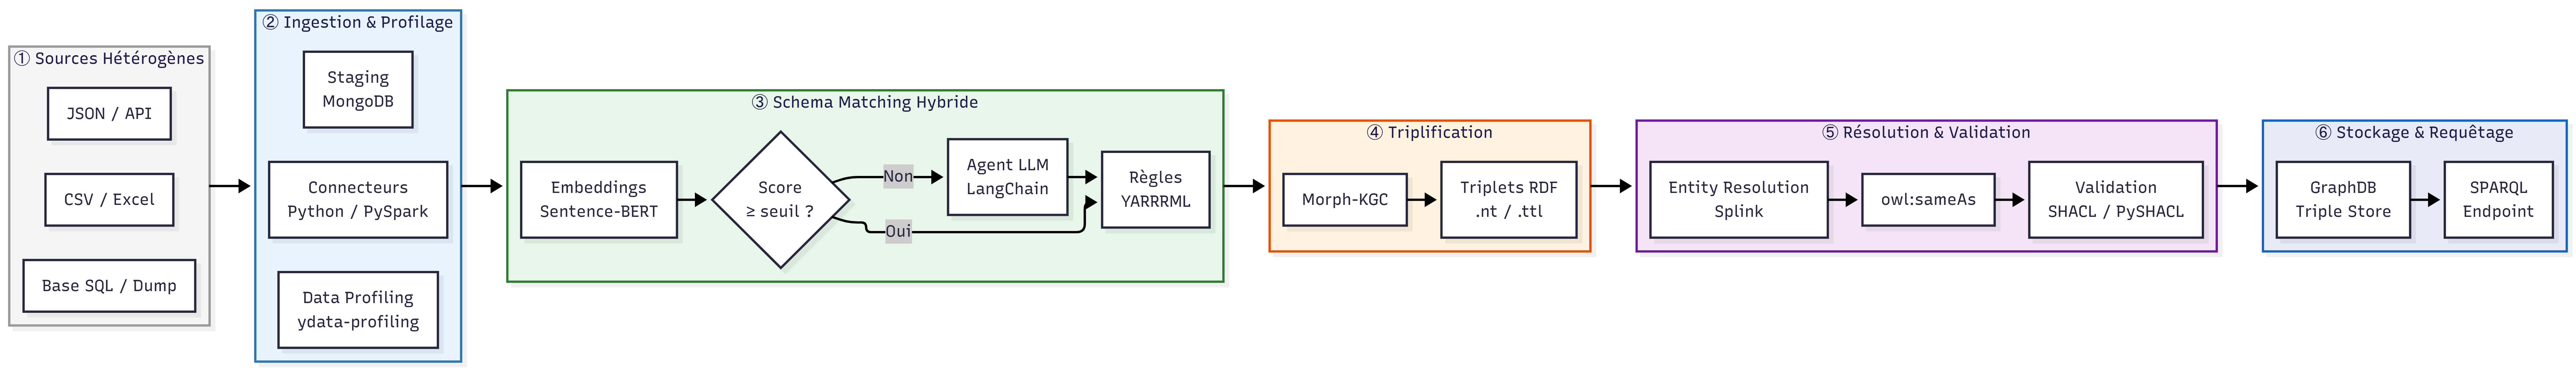
\includegraphics[width=\linewidth]{pics/Heterogeneous Data pipeline global.png}
%     \caption{Heterogeneous Data Pipeline Global}
%     \label{fig:heterogeneous-data-pipeline-global}
% \end{figure}

\begin{figure}[ht]
    \centering
    \resizebox{\textwidth}{!}{
    \begin{tikzpicture}[
        >=latex,
        % Styles des boîtes (textes plus grands grâce au changement d'échelle)
        box/.style    = {draw, rounded corners=5pt, align=center,
                         minimum height=1.2cm, font=\small,
                         text width=2.8cm},
        src/.style    = {box, fill=gray!8,        draw=gray!60},
        ing/.style    = {box, fill=blue!7,        draw=blue!50},
        mat/.style    = {box, fill=green!7,       draw=green!50!black},
        tri/.style    = {box, fill=orange!8,      draw=orange!70!black},
        res/.style    = {box, fill=violet!7,      draw=violet!60},
        sto/.style    = {box, fill=blue!10,       draw=blue!60!black},
        dec/.style    = {diamond, draw=green!50!black, fill=green!7,
                         align=center, font=\footnotesize,
                         inner sep=1pt, aspect=1.5},
        arr/.style    = {->, thick, draw=gray!70},
        % Style des grosses flèches entre les groupes (avec coins arrondis)
        grparr/.style = {->, line width=1.5pt, draw=blue!60, dashed, rounded corners=10pt},
    ]

    %% ════════════════ LIGNE 1 (EN HAUT) ════════════════

    %% ── Colonne 1 : Sources (X = 0) ──
    \node[src] (s1) at (0, 0)    {CSV / Excel};
    \node[src] (s2) at (0, -1.8) {Base SQL\\Dump};
    \node[src] (s3) at (0, -3.6) {JSON / API};

    \node[draw=gray!60, rounded corners, dashed, thick,
          fit=(s1)(s3), inner sep=6pt,
          label={[font=\small\bfseries]above:{\textcircled{1} Sources}}] (grp_src) {};

    %% ── Colonne 2 : Ingestion (X = 4.5) ──
    \node[ing] (i1) at (4.5, 0)    {Profiling\\ydata-profiling};
    \node[ing] (i2) at (4.5, -1.8) {Connecteurs\\Python/PySpark};
    \node[ing] (i3) at (4.5, -3.6) {Staging\\MongoDB};

    \node[draw=blue!50, rounded corners, dashed, thick,
          fit=(i1)(i2)(i3), inner sep=6pt,
          label={[font=\small\bfseries]above:{\textcircled{2} Ingestion}}] (grp_ing) {};

    %% ── Colonne 3 : Schema Matching (X = 9.0 et LLM à 12.8) ──
    \node[mat] (m1) at (9.0, 0)    {Sentence-BERT\\Embeddings};
    \node[dec] (md) at (9.0, -1.8) {Score\\$\geq \tau$ ?};
    \node[mat] (m4) at (9.0, -3.6) {Règles\\YARRRML};
    
    \node[mat] (m3) at (12.8, -1.8) {Agent LLM\\LangChain};

    \node[draw=green!50!black, rounded corners, dashed, thick,
          fit=(m1)(md)(m4)(m3), inner sep=6pt,
          label={[font=\small\bfseries]above:{\textcircled{3} Schema Matching}}] (grp_mat) {};


    %% ════════════════ LIGNE 2 (EN BAS) ════════════════
    
    %% ── Colonne 4 : Triplification (X = 0, Y = -8.0) ──
    \node[tri] (t1) at (0, -8.0) {Morph-KGC\\Moteur RML};
    \node[tri] (t2) at (0, -9.8) {Triplets RDF\\.nt / .ttl};

    \node[draw=orange!70!black, rounded corners, dashed, thick,
          fit=(t1)(t2), inner sep=6pt,
          label={[font=\small\bfseries]above:{\textcircled{4} Triplification}}] (grp_tri) {};

    %% ── Colonne 5 : Résolution (X = 4.5, Y = -8.0) ──
    \node[res] (r1) at (4.5, -8.0)  {Entity Res.\\Splink};
    \node[res] (r2) at (4.5, -9.8)  {\texttt{owl:sameAs}\\Fusion};
    \node[res] (r3) at (4.5, -11.6) {Validation\\SHACL};

    \node[draw=violet!60, rounded corners, dashed, thick,
          fit=(r1)(r2)(r3), inner sep=6pt,
          label={[font=\small\bfseries]above:{\textcircled{5} Résolution}}] (grp_res) {};

    %% ── Colonne 6 : Stockage (X = 9.0, Y = -8.0) ──
    \node[sto] (g1) at (9.0, -8.0) {GraphDB\\Triple Store};
    \node[sto] (g2) at (9.0, -9.8) {SPARQL\\Endpoint};

    \node[draw=blue!60!black, rounded corners, dashed, thick,
          fit=(g1)(g2), inner sep=6pt,
          label={[font=\small\bfseries]above:{\textcircled{6} Stockage}}] (grp_sto) {};


    %% ════════════════ FLUX ENTRE LES GROUPES ════════════════
    \draw[grparr] (grp_src.east) -- (grp_ing.west);
    \draw[grparr] (grp_ing.east) -- (grp_mat.west);
    
    % Flèche magique : relie la fin de la Ligne 1 au début de la Ligne 2
    % Part du Sud du groupe 3, descend, va à gauche jusqu'au groupe 4, puis descend
    \draw[grparr] (grp_mat.south) -- ++(0, -0.8) -| (grp_tri.north);

    \draw[grparr] (grp_tri.east) -- (grp_res.west);
    \draw[grparr] (grp_res.east) -- (grp_sto.west);

    %% ════════════════ FLUX INTERNES ════════════════
    % Schema Matching
    \draw[arr] (m1) -- (md);
    \draw[arr] (md) -- node[above, font=\footnotesize]{Non} (m3);
    \draw[arr] (md) -- node[right, font=\footnotesize]{Oui} (m4);
    \draw[arr] (m3.south) |- (m4.east);

    % Triplification
    \draw[arr] (t1) -- (t2);

    % Résolution
    \draw[arr] (r1) -- (r2);
    \draw[arr] (r2) -- (r3);

    % Stockage
    \draw[arr] (g1) -- (g2);

    \end{tikzpicture}
    } % Fin du resizebox
    
    \vspace{0.4cm}
    \caption{Architecture globale du pipeline de transformation structurée en deux phases. 
             La première ligne illustre l'ingestion et l'alignement sémantique hybride. 
             La seconde ligne détaille la génération RDF, la résolution d'entités et le stockage final.}
    \label{fig:pipeline_global}
\end{figure}



Le pipeline est composé de \textbf{cinq modules fonctionnels} complétés par
une infrastructure d'orchestration transverse (Docker Compose,
section~\ref{sec:docker}). Chaque module répond à une problématique
spécifique de l'intégration de données hétérogènes, et son artefact de
sortie constitue l'artefact d'entrée du module suivant, sans état partagé
implicite entre les étapes.

\begin{itemize}
    \item \textbf{Module 1 — Ingestion et prétraitement}
          (section~\ref{sec:module_ingestion}) : collecte des sources
          brutes hétérogènes (CSV, Excel, SQL, JSON), profilage
          automatique de la qualité, normalisation syntaxique et
          persistance dans une zone de staging MongoDB. Il traite
          exclusivement l'hétérogénéité \textit{structurelle} et
          \textit{syntaxique}.
    \item \textbf{Module 2 — Schema matching hybride}
          (section~\ref{sec:module_matching}) : identification de la
          propriété ontologique correspondant à chaque colonne source,
          par une cascade SBERT (rapide, déterministe) puis agent LLM
          (coûteux, réservé aux cas ambigus), et génération automatique
          des règles de mapping YARRRML. C'est le module qui résout
          l'hétérogénéité \textit{sémantique}, la plus difficile des
          trois.
    \item \textbf{Module 3 — Triplification}
          (section~\ref{sec:module_triplification}) : exécution
          déclarative des règles YARRRML par le moteur Morph-KGC,
          produisant les triplets RDF conformes à l'ontologie cible.
    \item \textbf{Module 4 — Résolution d'entités et validation}
          (section~\ref{sec:module_validation}) : réconciliation
          probabiliste des entités décrites par plusieurs sources
          (Splink), génération des ponts \texttt{owl:sameAs}, puis
          validation structurelle du graphe par des contraintes SHACL.
    \item \textbf{Module 5 — Stockage et requêtage} : chargement du
          graphe validé dans un triple store (GraphDB) exposant un
          point d'accès SPARQL, ainsi qu'une interface de visualisation
          interactive.
\end{itemize}

\noindent L'ensemble de ces modules est orchestré par
\textbf{Docker Compose} (section~\ref{sec:docker}), qui garantit que le
pipeline complet est déployable en une seule commande, indépendamment de
l'infrastructure hôte — répondant directement au déficit de
reproductibilité identifié au chapitre~\ref{chap:etat_art}.

Le tableau~\ref{tab:artefacts} synthétise les artefacts d'entrée et de sortie
de chaque module, matérialisant l'interface contractuelle entre les étapes
successives du pipeline.

\begin{table}[ht]
\centering
\caption{Artefacts d'entrée et de sortie de chaque module du pipeline.}
\label{tab:artefacts}
\renewcommand{\arraystretch}{1.35}
\begin{tabular}{|p{0.5cm}|p{3.2cm}|p{4.2cm}|p{4.2cm}|}
\hline
\textbf{\#} & \textbf{Module} & \textbf{Entrée} & \textbf{Sortie} \\
\hline
1 & Ingestion \& Profilage
  & Fichiers CSV, Excel, dumps SQL, JSON bruts
  & DataFrames normalisés, rapports de profilage,
    collections MongoDB de staging \\
\hline
2 & Schema Matching Hybride
  & Schémas sources (noms et exemples de colonnes),
    ontologie OWL cible
  & Règles de mapping YARRRML validées par module \\
\hline
3 & Triplification
  & Données normalisées + règles YARRRML
  & Fichiers de triplets RDF (format N-Triples \texttt{.nt}
    ou Turtle \texttt{.ttl}) \\
\hline
4 & Résolution d'entités \& Validation
  & Triplets RDF + contraintes SHACL + ontologie OWL
  & Graphe RDF enrichi (\texttt{owl:sameAs}),
    rapport de validation SHACL \\
\hline
5 & Stockage \& Requêtage
  & Graphe RDF validé
  & Repository GraphDB peuplé, endpoint SPARQL opérationnel \\
\hline
\end{tabular}
\end{table}

% ─────────────────────────────────────────────────────────────
\section{Module 1 : Ingestion et Prétraitement des Données}
\label{sec:module_ingestion}
% ─────────────────────────────────────────────────────────────

\subsection{Rôle fonctionnel}

Le module d'ingestion constitue le point d'entrée du pipeline.
Son rôle est de collecter les données brutes provenant de sources hétérogènes,
de les normaliser dans un format interne unifié, d'en évaluer la qualité, et de
les persister dans une zone de staging avant les traitements sémantiques.
Ce module n'effectue aucune transformation sémantique : son périmètre est
strictement limité à l'hétérogénéité \textit{structurelle} et \textit{syntaxique}
telle que définie dans la taxonomie présentée à la section~\ref{sec:construction_auto}.

\subsection{Sources supportées et stratégie de scalabilité}
\label{subsec:sources}

Le pipeline supporte nativement les formats tabulaires les plus
répandus dans les environnements industriels et académiques :
\begin{itemize}
    \item \textbf{Fichiers plats} : CSV (séparateurs variables,
          encodages UTF-8 et Latin-1), Excel (\texttt{.xlsx} et
          \texttt{.xls}), fichiers TSV à tabulations.
    \item \textbf{Bases relationnelles} : connexion via des dumps SQL
          (\texttt{.sql}) ou via des connecteurs SQLAlchemy~\cite{bayer2012sqlalchemy}
          vers PostgreSQL, MySQL et SQLite.
    \item \textbf{Formats semi-structurés} : JSON tabulaire (tableaux
          d'objets), XML avec structure répétitive extractible.
\end{itemize}

\paragraph{Stratégie de scalabilité : bascule Pandas / PySpark.}
Chaque connecteur est implémenté selon une stratégie à deux niveaux,
afin de couvrir un spectre de volumes allant de quelques milliers à
plusieurs millions d'enregistrements :
\begin{itemize}
    \item \textbf{Mode Pandas}~\cite{pandas2020} :
          utilisé lorsque la taille estimée du fichier source est
          inférieure à un seuil configurable (valeur par défaut :
          \textbf{500 Mo} ou \textbf{$10^6$ lignes}).
          Dans ce mode, l'intégralité des données est chargée en
          mémoire vive, ce qui offre les meilleures performances
          pour les petits volumes grâce à la vectorisation NumPy.
    \item \textbf{Mode PySpark}~\cite{zaharia2016spark} :
          activé automatiquement lorsque la taille dépasse le seuil
          ou lorsque le paramètre \texttt{force\_spark=True} est
          positionné dans la configuration du pipeline.
          PySpark traite les données en partitions distribuées,
          permettant de dépasser les contraintes de mémoire d'un
          seul nœud et d'exploiter un cluster multi-nœuds si
          disponible.
\end{itemize}

La détection automatique du mode est réalisée par un module de
\textbf{profilage léger pré-ingestion} : avant le chargement
complet, seules les métadonnées du fichier (taille en octets,
nombre de lignes estimé par échantillonnage des premiers et derniers
blocs) sont lues, ce qui permet de choisir le moteur approprié
sans charger l'ensemble des données en mémoire.
Dans les deux modes, le résultat produit est un
\textit{DataFrame} dont l'interface est unifiée via une couche
d'abstraction, garantissant que les modules aval (profilage,
normalisation, schema matching) sont indépendants du moteur
d'exécution utilisé.

\subsection{Profilage automatique des données}

Dès l'ingestion, chaque source fait l'objet d'un \textbf{profilage automatique}
via la bibliothèque \texttt{ydata-profiling}~\cite{ydataprofiling2023}.
Ce profilage produit pour chaque colonne : son type inféré (numérique, catégoriel,
temporel, textuel), sa cardinalité, son taux de valeurs manquantes, sa
distribution statistique (quartiles, histogramme), et des exemples de valeurs
représentatives.

Ces métadonnées de profilage jouent un rôle crucial dans le module suivant :
elles constituent la \textbf{représentation augmentée de colonne} transmise
au module de schema matching, permettant au module SBERT et à l'agent LLM de
disposer d'un contexte plus riche que le seul nom de la colonne.

\subsection{Staging et Mapping Store dans MongoDB}
\label{subsec:mongodb}

Les DataFrames normalisés sont persistés dans une base
\textbf{MongoDB}~\cite{mongodb2024} utilisée selon deux rôles
complémentaires dans le pipeline.

\paragraph{Rôle 1 — Zone de staging des données.}
MongoDB sert de \textbf{zone de staging intermédiaire} entre le
module d'ingestion et le module de schema matching.
Son schéma flexible (document JSON sans DDL préalable) permet de
stocker des DataFrames de formats hétérogènes dans des collections
séparées, sans migration de schéma.
Chaque collection correspond à une source et contient, en plus
des données normalisées, les métadonnées de profilage
(type inféré, cardinalité, taux de nullité, exemples de valeurs)
sous forme de sous-documents JSON.
Cette co-localisation des données et de leurs métadonnées dans un
même store simplifie l'accès par le module de schema matching,
qui peut requêter simultanément le contenu et le profil d'une
colonne.

\paragraph{Rôle 2 — Mapping Store versionné.}
MongoDB remplit un second rôle, moins courant dans la littérature
mais crucial pour la reproductibilité du pipeline :
il sert de \textbf{mapping store versionné}, c'est-à-dire d'un
référentiel persistant des règles de mapping YARRRML produites
par le module de schema matching.

Chaque règle de mapping est stockée dans une collection dédiée
(\texttt{schema\_mappings}) sous la forme d'un document comprenant :
\begin{itemize}
    \item L'identifiant de la source et le nom de la colonne.
    \item La propriété ontologique cible et le type XSD mappé.
    \item La voie de décision empruntée (\texttt{"sbert"} ou
          \texttt{"llm"}).
    \item Le score de confiance associé.
    \item Un \textbf{horodatage} et un \textbf{identifiant de version}
          permettant de tracer l'historique des modifications.
    \item Un indicateur de validation humaine (\texttt{validated: true/false}).
\end{itemize}

Cette architecture de mapping store présente deux avantages
majeurs.
Premièrement, elle permet de \textbf{réutiliser les règles validées}
lors d'une exécution ultérieure du pipeline sur la même source,
sans relancer le module de schema matching.
Deuxièmement, elle offre un mécanisme de \textbf{révision humaine
incrémentale} : un expert métier peut consulter et valider les
correspondances via une interface dédiée, et les règles invalidées
sont automatiquement soumises à une nouvelle analyse LLM lors de
la prochaine exécution.
Ce paradigme est aligné avec les recommandations
\textit{human-in-the-loop} de la littérature récente sur
l'automatisation du schema matching~\cite{branco2025integration}.

\subsection{Normalisation syntaxique}

Avant la persistance en staging, un module de normalisation syntaxique applique
une série de transformations canoniques sur les valeurs :
\begin{itemize}
    \item \textbf{Dates} : toutes les dates sont converties vers le format
          ISO 8601 (\texttt{YYYY-MM-DD}), indépendamment du format source
          (\texttt{DD/MM/YYYY}, \texttt{MM-DD-YY}, \texttt{Jan 15, 2024},
          etc.), en s'appuyant sur la bibliothèque \texttt{dateutil}~\cite{dateutil2024}.
    \item \textbf{Nombres} : unification des séparateurs décimaux et de milliers,
          suppression des symboles monétaires, conversion vers \texttt{float64}.
    \item \textbf{Textes} : normalisation Unicode (NFC), homogénéisation de la
          casse, suppression des espaces superflus.
    \item \textbf{Valeurs nulles} : détection et remplacement cohérent des
          représentations variées du vide (\texttt{"N/A"}, \texttt{"null"},
          cellule vide, \texttt{"-"}).
\end{itemize}
Ces normalisations syntaxiques réduisent directement l'hétérogénéité de niveau 2
(syntaxique) avant que les données n'atteignent le moteur de triplification, où
elles seront typées explicitement via les types XSD de RDF.

\medskip
Une fois les données ingérées, normalisées et persistées dans la zone de
staging MongoDB, le pipeline dispose d'une représentation structurellement
homogène de sources initialement hétérogènes. La question qui se pose alors
est d'ordre sémantique~: comment identifier automatiquement la propriété
ontologique vers laquelle chaque colonne doit être mappée~? C'est l'objet
du Module~2, présenté dans la section suivante.

% ─────────────────────────────────────────────────────────────
\section{Module 2 : Schema Matching Hybride et Génération YARRRML}
\label{sec:module_matching}
% ─────────────────────────────────────────────────────────────

Ce module constitue le \textbf{cœur scientifique} de la contribution présentée
dans ce mémoire.
Son objectif est de résoudre l'hétérogénéité sémantique --- la plus difficile des
trois formes d'hétérogénéité --- en identifiant automatiquement la correspondance
entre chaque colonne d'une source tabulaire et la propriété ontologique adéquate
de l'ontologie OWL cible, puis en formalisant cette correspondance dans une règle
de mapping YARRRML prête à être exécutée par Morph-KGC.

\subsection{Représentation des colonnes sources}

L'entrée de ce module n'est pas simplement le nom d'une colonne, mais une
\textbf{représentation augmentée} composée de :
\begin{itemize}
    \item Le \textbf{nom de la colonne} (\textit{header}) tel qu'extrait de
          la source.
    \item Le \textbf{type inféré} et la \textbf{distribution statistique} issus
          du profilage (section~\ref{sec:module_ingestion}).
    \item Trois à cinq \textbf{exemples de valeurs} représentatives de la colonne.
    \item Le \textbf{nom de la table source} et, le cas échéant, les noms des
          colonnes adjacentes (contexte structurel local).
\end{itemize}
Cette représentation augmentée permet de discriminer deux colonnes portant le
même nom mais appartenant à des tables de domaines différents (par exemple,
une colonne \texttt{date} dans une table de commandes et une colonne \texttt{date}
dans une table de naissances).

% À insérer comme nouvelle sous-section entre 2.4.1 et 2.4.2
\subsection{L'ontologie du domaine : artefact central du pipeline}
\label{subsec:ontologie}

Avant de décrire le processus d'alignement, il est nécessaire
de préciser la nature et la structure de l'\textbf{ontologie OWL
cible} vers laquelle toutes les colonnes sources sont mappées.
Cette ontologie constitue l'artefact sémantique fondateur du
pipeline : elle définit le vocabulaire partagé qui permet d'unifier
des sources hétérogènes sous un modèle de connaissance commun.

\paragraph{Conception et structure.}
L'ontologie du domaine est modélisée sous
\textbf{Protégé}~\cite{musen2015protege} (version 5.x),
le standard académique et industriel pour la création d'ontologies
OWL 2 DL.
Elle suit le principe de \textbf{réutilisation maximale} :
les classes et propriétés des vocabulaires standards du Web
Sémantique sont réutilisées chaque fois que possible, et
complétées par des éléments spécifiques au domaine préfixés
\texttt{ex:} (\texttt{http://kg.projet.fr/ontology\#}).

Les vocabulaires réutilisés sont les suivants :
\begin{itemize}
    \item \textbf{FOAF} (\textit{Friend of a Friend})~\cite{foaf2014} :
          pour les personnes (\texttt{foaf:Person}),
          leurs noms (\texttt{foaf:familyName},
          \texttt{foaf:firstName}) et leurs emails
          (\texttt{foaf:mbox}).
    \item \textbf{Schema.org}~\cite{guha2016schemaorg} :
          pour les dates de naissance (\texttt{schema:birthDate}),
          les organisations (\texttt{schema:Organization})
          et les transactions (\texttt{schema:Order}).
    \item \textbf{Dublin Core}~\cite{weibel1998dublin} :
          pour les métadonnées descriptives des sources
          (\texttt{dc:title}, \texttt{dc:source}).
\end{itemize}

L'ontologie compte, dans sa version utilisée pour les expériences
de ce travail, \textbf{12 classes}, \textbf{34 propriétés d'objet}
et \textbf{28 propriétés de données}, couvrant les domaines
de la gestion de la relation client (CRM) et des ressources humaines
(RH), qui correspondent aux sources de données utilisées pour
l'évaluation (voir chapitre~\ref{chap:evaluation}).
Elle est exportée au format Turtle (\texttt{.ttl}) et versionnée
dans le dépôt Git du projet.

\paragraph{Alignement avec OWL 2 DL.}
Le profil OWL 2 DL est retenu pour sa garantie de
\textbf{décidabilité du raisonnement}~\cite{hogan2021knowledge} :
un moteur de raisonnement (HermiT~\cite{shearer2008hermit} dans notre cas)
peut déterminer en temps fini toutes les conséquences logiques de
l'ontologie, notamment les relations d'équivalence entre entités
issues de sources différentes déclarées via
\texttt{owl:equivalentProperty} et \texttt{owl:sameAs}.
Cette propriété est exploitée dans le module de résolution d'entités
décrit à la section~\ref{sec:module_validation}.

\subsection{Approche symbolique : embeddings Sentence-BERT}
\label{subsec:sbert}

La première couche du module de matching est une approche
\textbf{symbolique déterministe} basée sur les embeddings
sémantiques produits par le modèle
Sentence-BERT~\cite{reimers2019sbert}.

Plus précisément, nous utilisons le modèle pré-entraîné \\
\texttt{paraphrase-multilingual-MiniLM-L12-v2}, disponible via la
bibliothèque \\ \texttt{sentence-transformers}~\cite{reimers2019sbert}.
Ce choix est motivé par deux critères complémentaires.
D'une part, ce modèle est conçu pour optimiser la similarité cosinus
comme mesure de proximité sémantique, contrairement aux modèles
BERT originaux dont les représentations ne sont pas directement
comparables via cosinus~\cite{reimers2019sbert}.
D'autre part, sa variante multilingue couvre plus de cinquante
langues, ce qui le rend adapté aux contextes industriels dans lesquels
les colonnes sources peuvent être libellées en français, en anglais
ou dans d'autres langues simultanément.

\paragraph{Processus d'encodage et calcul de similarité.}
Le processus est le suivant :
\begin{enumerate}
    \item Chaque colonne source est encodée en un vecteur dense de
          dimension $d = 384$ à partir de sa représentation augmentée
          (nom de la colonne, type inféré, exemples de valeurs).
    \item Chaque propriété de l'ontologie OWL cible est encodée de la
          même façon, en concaténant son URI locale, son
          \texttt{rdfs:label} et son \texttt{rdfs:comment} en une
          seule chaîne textuelle avant l'encodage.
    \item La \textbf{similarité cosinus} entre chaque vecteur de
          colonne source et chaque vecteur de propriété cible est
          calculée, produisant une matrice de scores
          $S \in [0, 1]^{n_s \times n_p}$, où $n_s$ est le nombre de
          colonnes sources et $n_p$ le nombre de propriétés de
          l'ontologie.
    \item Si le score maximal $s^* = \max_j S_{ij}$ pour la
          colonne $i$ dépasse un seuil $\tau$, la correspondance est
          acceptée automatiquement et la règle YARRRML correspondante
          est générée sans intervention du LLM.
\end{enumerate}

\paragraph{Calibration du seuil $\tau$.}
La valeur du seuil $\tau$ est un hyperparamètre critique du module :
une valeur trop basse génère des correspondances incorrectes
(faux positifs), tandis qu'une valeur trop haute renvoie
inutilement des cas simples vers le LLM, augmentant le coût
computationnel. La valeur par défaut retenue pour ce travail est
$\tau = 0.82$, déterminée par une procédure de calibration sur un
\textbf{gold standard annoté manuellement}.

Cette procédure consiste à calculer le F1-score du module SBERT seul
(sans LLM) pour des valeurs de $\tau$ variant entre $0.60$ et $0.95$
par pas de $0.02$, sur l'ensemble d'entraînement du gold standard.
La valeur $\tau = 0.82$ correspond au maximum du F1-score observé sur
cet ensemble, indiquant le meilleur compromis entre précision (peu de
faux positifs) et rappel (peu de cas simples renvoyés inutilement au
LLM). Les résultats complets de cette calibration, incluant la courbe
F1-score en fonction de $\tau$, sont présentés au
chapitre~\ref{chap:evaluation}.

Cette approche déterministe traite efficacement les cas de
correspondance à forte similarité sémantique (par exemple,
\texttt{nom\_complet} $\rightarrow$ \texttt{foaf:name},
\texttt{email\_professionnel} $\rightarrow$ \texttt{foaf:mbox})
avec un coût computationnel négligeable, de l'ordre de la
milliseconde par paire sur un processeur standard, sans appel API
externe.


\subsection{Approche neuronale : agent LLM via LangChain}
\label{subsec:llm_agent}

Pour les colonnes dont le score SBERT est inférieur au seuil $\tau$,
le pipeline délègue la décision à un \textbf{agent LLM} orchestré
par le framework LangChain~\cite{langchain2023}.
Ce sont typiquement les cas d'hétérogénéité sémantique profonde,
où deux termes désignent le même concept sans partager aucun token
lexical (par exemple, \texttt{CA\_annuel}
$\rightarrow$ \texttt{ex:annualRevenue}).

\paragraph{Choix du modèle de langage.}
LangChain est un framework d'orchestration qui abstrait la couche
d'appel au modèle de langage sous-jacent.
Dans ce travail, le modèle utilisé est \textbf{GPT-4o}
(OpenAI)~\cite{openai2024gpt4}, qui présente les avantages
suivants par rapport aux alternatives évaluées
(Mistral-7B-Instruct~\cite{jiang2023mistral} et
LLaMA-3-8B~\cite{touvron2023llama}) :
\begin{itemize}
    \item \textbf{Précision sur les tâches de raisonnement structural} :
          GPT-4o démontre une capacité supérieure à interpréter le
          contexte sémantique d'une colonne à partir d'exemples de
          valeurs, tâche qui requiert un raisonnement combiné sur le
          nom, le type et le contenu de la colonne.
    \item \textbf{Fiabilité du format de sortie JSON} :
          GPT-4o supporte nativement le mode
          \textit{structured output}~\cite{openai2024gpt4},
          qui garantit que la réponse est un objet JSON
          syntaxiquement valide conforme à un schéma prédéfini,
          éliminant les erreurs de parsing.
    \item \textbf{Latence acceptable} :
          le temps de réponse moyen observé est de l'ordre de
          1 à 3 secondes par requête, compatible avec un usage
          en mode batch sur des dizaines à quelques centaines de
          colonnes ambiguës.
\end{itemize}

Il convient de souligner que le coût d'appel API de GPT-4o constitue
la principale limite de cette approche pour des pipelines à très
grand nombre de colonnes.
C'est précisément la raison pour laquelle le LLM n'est sollicité
qu'en dernier recours, après le filtrage par le module SBERT.
L'architecture hybride permet de limiter le nombre d'appels LLM
au strict minimum des cas ambigus.
La conception du pipeline est par ailleurs compatible avec un
remplacement de GPT-4o par un modèle open-source déployé localement
(Mistral ou LLaMA via Ollama~\cite{ollama2024}) pour les contextes
où la confidentialité des données est une contrainte, sans
modification de l'architecture LangChain.

\paragraph{Structure du prompt.}
L'agent LangChain reçoit un prompt structuré en plusieurs sections :
\begin{itemize}
    \item \textbf{Contexte du domaine} : description de l'ontologie
          cible et de ses classes principales.
    \item \textbf{Description de la colonne source} : nom, type,
          distribution statistique, et trois à cinq exemples de
          valeurs représentatives.
    \item \textbf{Propriétés cibles candidates} : liste des propriétés
          de l'ontologie dont le score SBERT se situe entre
          $\tau - 0.15$ et $\tau$ (zone d'ambiguïté), avec leurs
          définitions \texttt{rdfs:label} et \texttt{rdfs:comment}.
    \item \textbf{Exemples \textit{few-shot}} :
          deux à trois exemples de mappings corrects issus du gold
          standard, présentant des cas similaires d'équivalence
          sémantique sans similarité lexicale.
    \item \textbf{Instruction de sortie} :
          spécification du schéma JSON attendu en sortie, comprenant
          la propriété cible retenue, le score de confiance estimé
          (entre 0 et 1), la transformation XSD à appliquer, et une
          justification textuelle en une phrase.
\end{itemize}

\paragraph{Gestion des erreurs et mécanisme de retry.}
La sortie JSON de l'agent est parsée et validée structurellement
avant d'être utilisée pour générer la règle YARRRML correspondante.
En cas d'incohérence (sortie non conforme au schéma JSON attendu
ou propriété cible non reconnue dans l'ontologie), un mécanisme
de \textit{retry} avec reformulation automatique du prompt est
déclenché, avec un maximum de trois tentatives.
Si les trois tentatives échouent, la colonne est marquée comme
\textit{non réconciliée} et consignée dans un rapport d'anomalies
structuré (format JSON) pour révision humaine, incluant le nom
de la colonne, les scores SBERT des candidats proches, et les
sorties brutes des tentatives LLM.


\subsection{Architecture hybride et seuil adaptatif}

La figure~\ref{fig:schema_matching_detail} illustre le flux de décision du
module de schema matching hybride.
L'articulation entre le module SBERT et l'agent LLM constitue une stratégie
de \textbf{cascade de coûts croissants} : le traitement le moins coûteux
(inférence SBERT locale, de l'ordre de la milliseconde par paire) est tenté
en premier, et le traitement le plus coûteux (appel API LLM, de l'ordre de
la seconde par requête) n'est sollicité que pour les cas que le premier
niveau ne peut résoudre avec confiance.

\begin{figure}[ht]
    \centering
    \resizebox{\textwidth}{!}{
    \begin{tikzpicture}[
        >=latex,
        % Styles des boîtes
        box/.style={draw=gray!80, rounded corners=4pt, align=center,
                    minimum height=1.1cm, font=\small,
                    text width=3.2cm},
        dec/.style={diamond, draw=green!60!black, fill=green!8, 
                    align=center, font=\footnotesize, 
                    inner sep=1pt, aspect=1.8},
        arr/.style={->, thick, draw=gray!80},
        % Styles de couleurs spécifiques
        ok/.style ={draw=green!60!black, fill=green!8},
        llm/.style={draw=orange!80!black, fill=orange!8},
        err/.style={draw=red!60, fill=red!8},
    ]
        
        %% ── Nœuds avec coordonnées absolues ──
        
        \node[box]      (col)    at (0, 0)     {Colonne source\\(repr. augmentée)};
        \node[box, ok]  (sbert)  at (4.5, 0)   {Sentence-BERT\\Embedding};
        \node[dec]      (thresh) at (8.5, 0)   {Score\\$s^* \geq \tau$ ?};
        
        % Branche du Haut (Oui)
        \node[box, ok]  (yarrml) at (12.5, 2)  {Règle\\YARRRML};
        
        % Branche du Bas (Non)
        \node[box, llm] (llm)    at (12.5, -2) {Agent LLM\\(LangChain)};
        \node[dec]      (valid)  at (16.5, -2) {JSON\\valide ?};
        
        % Sous-branches de la validation
        \node[box, ok]  (yar2)   at (20.5, 0)  {Règle\\YARRRML};
        \node[box, err] (err)    at (20.5, -4) {Anomalie\\(révision humaine)};

        %% ── Flèches de connexion orthogonales ──
        
        \draw[arr] (col)   -- (sbert);
        \draw[arr] (sbert) -- (thresh);
        
        % Depuis le premier test (Seuil SBERT)
        % |- signifie "aller à la verticale puis à l'horizontale"
        \draw[arr] (thresh.north) |- node[above left, font=\footnotesize, text=green!60!black]{Oui} (yarrml.west);
        \draw[arr] (thresh.south) |- node[below left, font=\footnotesize, text=orange!80!black]{Non} (llm.west);
        
        \draw[arr] (llm) -- (valid);
        
        % Depuis le second test (Validation JSON)
        \draw[arr] (valid.north) |- node[above left, font=\footnotesize, text=green!60!black]{Oui} (yar2.west);
        \draw[arr] (valid.south) |- node[below left, font=\footnotesize, text=red!80]{Non} (err.west);

    \end{tikzpicture}
    } % Fin du resizebox
    
    \vspace{0.3cm}
    \caption{Flux de décision du module de schema matching hybride.
             Le seuil $\tau$ est calibré empiriquement sur le gold standard
             pour maximiser le F1-score global du module.}
    \label{fig:schema_matching_detail}
\end{figure}

\subsection{Génération automatique des règles YARRRML}

Quelle que soit la voie empruntée (SBERT ou LLM), le résultat du module de
matching est une règle de mapping au format \textbf{YARRRML}.
YARRRML (\textit{Yet Another RDF Mapper}), déjà justifié dans
l'état de l'art~\cite{warren2024yarrrml}, est utilisé ici pour deux raisons
complémentaires.
D'une part, sa syntaxe YAML est lisible et modifiable par un expert métier non
informaticien, ce qui facilite la phase de validation humaine des mappings.
D'autre part, YARRRML est compilable vers des fichiers RML standard, exécutables
par le moteur Morph-KGC sans modification supplémentaire.

Un exemple de règle YARRRML générée automatiquement par le pipeline pour une
source de données clients est présenté ci-dessous :

\begin{verbatim}
prefixes:
  ex:   "http://kg.projet.fr/ontology#"
  foaf: "http://xmlns.com/foaf/0.1/"
  xsd:  "http://www.w3.org/2001/XMLSchema#"

mappings:
  clients_source_A:
    sources: [["clients_A.csv~csv"]]
    s: ex:Customer_$(ID_Client)
    po:
      - [rdf:type, foaf:Person]
      - [foaf:familyName, $(nom_complet), xsd:string]
      - [foaf:mbox, $(email_pro), xsd:anyURI]
      - [ex:annualRevenue, $(CA_annuel), xsd:decimal]
      - [schema:birthDate, $(dt_naissance), xsd:date]
\end{verbatim}

Chaque triplet \texttt{po} (Predicate-Object) est la traduction directe d'une
correspondance identifiée par le module de schema matching : la colonne source
(\texttt{\$(nom\_complet)}) est associée à la propriété ontologique
(\texttt{foaf:familyName}) avec son type XSD cible (\texttt{xsd:string}).

% ─────────────────────────────────────────────────────────────
\section{Module 3 : Triplification Sémantique avec Morph-KGC}
\label{sec:module_triplification}
% ─────────────────────────────────────────────────────────────

\subsection{Rôle fonctionnel}

Le module de triplification transforme les données normalisées en
staging, guidé par les règles YARRRML produites par le module précédent,
en un ensemble de \textbf{triplets RDF} conformes à l'ontologie cible.
C'est l'étape qui matérialise concrètement le passage de la représentation
tabulaire à la représentation graphe.

\subsection{Justification du choix de Morph-KGC}

Le moteur retenu pour l'exécution des règles RML est
\textbf{Morph-KGC}~\cite{arenas2023morphkgc}, développé en Python par
l'équipe d'Arenas-Guerrero et al. (ESWC 2023).
Ce choix est justifié par plusieurs arguments complémentaires par rapport
aux alternatives disponibles (RMLMapper en Java, RDFLib-applet en Python,
triplification manuelle par script).

Premièrement, Morph-KGC est nativement intégrable dans un pipeline Python
sans dépendance JVM, ce qui simplifie l'environnement d'exécution Docker.
Deuxièmement, il supporte les \textbf{fonctions de transformation définies
par l'utilisateur} (\textit{user-defined functions}, UDFs), permettant
d'appliquer des transformations syntaxiques complexes (nettoyage de chaînes,
normalisation de dates, casting de types) directement dans les règles RML,
sans prétraitement séparé.
Troisièmement, sa conception orientée flux (\textit{streaming}) lui permet
de traiter de grands volumes de données sans charger l'intégralité du jeu
de données en mémoire, répondant ainsi à la contrainte de scalabilité
Big Data~\cite{arenas2023morphkgc}.
Quatrièmement, par rapport à un script Python natif utilisant directement
la bibliothèque RDFLib~\cite{rdflib2022}, l'approche déclarative de
Morph-KGC sépare la logique de transformation du code d'exécution :
modifier une règle de mapping ne nécessite pas de modifier le code Python
du pipeline, ce qui améliore la maintenabilité et la testabilité.

\subsection{Processus d'exécution}

L'exécution de Morph-KGC est pilotée par un fichier de configuration INI
qui référence les sources de données, les fichiers de règles YARRRML compilés
en RML, et le format de sortie souhaité.
Deux formats de sortie sont supportés dans notre pipeline :
\begin{itemize}
    \item \textbf{N-Triples} (\texttt{.nt}) : un triplet par ligne, format
          optimal pour le traitement en flux et l'import dans les triple stores.
    \item \textbf{Turtle} (\texttt{.ttl}) : format plus compact et lisible
          par un humain, utilisé pour l'inspection manuelle et la documentation.
\end{itemize}

\subsection{Gestion des graphes nommés}

Pour maintenir la \textbf{traçabilité de la provenance} des triplets générés
depuis des sources multiples, Morph-KGC est configuré pour produire des
\textbf{N-Quads} (\texttt{.nq}) plutôt que des N-Triples lors du traitement
multi-sources.
Chaque triplet est associé à un graphe nommé correspondant à la source dont il
est issu (par exemple,\\  \texttt{<http://kg.projet.fr/graph/source\_A>}).
Cette granularité de provenance facilite l'audit de qualité et la détection
d'incohérences inter-sources dans l'étape suivante.

\medskip
À l'issue de la triplification, le graphe RDF produit est sémantiquement
conforme à l'ontologie cible au niveau des propriétés individuelles. Il
peut cependant contenir deux classes de défauts résiduels~: des entités
redondantes issues de sources multiples représentant le même individu réel,
et des violations de contraintes structurelles définies par l'ontologie. Le
Module~4, présenté dans la section suivante, adresse ces deux classes de
défauts de manière séquentielle et complémentaire.

% ─────────────────────────────────────────────────────────────
\section{Module 4 : Résolution d'Entités et Validation SHACL}
\label{sec:module_validation}
% ─────────────────────────────────────────────────────────────

Ce module opère en deux phases distinctes mais complémentaires :
la résolution d'entités, qui fusionne les représentations redondantes d'une
même entité du monde réel issues de sources différentes, et la validation SHACL,
qui vérifie la conformité formelle du graphe produit à l'ontologie cible.

\subsection{Phase 1 — Résolution d'entités avec Splink}

\subsubsection{Problématique}
Après triplification, le graphe contient potentiellement plusieurs nœuds RDF
distincts représentant la même entité réelle.
Par exemple, le client \textit{Jean Dupont} peut apparaître sous l'URI
\texttt{ex:Customer\_42} issue du système CRM et sous l'URI
\texttt{ex:Customer\_E17} issue du système RH, avec des attributs partiellement
redondants et partiellement complémentaires.
La résolution d'entités (\textit{entity resolution} ou \textit{record linkage})
vise à identifier ces paires et à les fusionner sémantiquement.

\subsubsection{Approche : Splink}
Le pipeline utilise la bibliothèque \textbf{Splink}~\cite{splink2023},
développée par le Ministère de la Justice britannique, pour la résolution
d'entités probabiliste.
Splink implémente le modèle de Fellegi-Sunter~\cite{fellegi1969theory},
dans lequel chaque paire de candidats à la fusion reçoit un score de
correspondance calculé à partir d'une combinaison pondérée de comparaisons
attribut par attribut.

Le processus comporte trois étapes :
\begin{enumerate}
    \item \textbf{Blocking} : pour éviter la comparaison cartésienne de toutes
          les paires possibles (complexité $O(n^2)$), un mécanisme de
          \textit{blocking} regroupe les enregistrements candidats selon des
          clés de blocage (par exemple, première lettre du nom de famille,
          code postal).
          Seules les paires au sein d'un même bloc sont comparées,
          réduisant drastiquement le nombre de comparaisons.
    \item \textbf{Scoring} : pour chaque paire candidate, Splink calcule un
          score de correspondance basé sur des comparaisons multi-attributs :
          similarité de Jaro-Winkler~\cite{winkler1990string} sur les noms,
          correspondance exacte sur les emails, distance de Levenshtein sur
          les adresses.
    \item \textbf{Classification} : les paires dont le score dépasse un seuil
          de décision $\lambda$ (calibré sur le gold standard) sont classifiées
          comme \textit{match} (même entité réelle) et génèrent un triplet
          \texttt{owl:sameAs} reliant leurs deux URIs dans le graphe.
\end{enumerate}

\subsubsection{Génération des triplets \texttt{owl:sameAs}}
Chaque paire classifiée comme \textit{match} produit le triplet RDF suivant,
qui est ajouté au graphe :

\begin{center}
\texttt{<ex:Customer\_42> owl:sameAs <ex:Customer\_E17>}
\end{center}

Ce triplet est exploitable par les raisonneurs OWL : grâce à la sémantique de
\texttt{owl:sameAs}, tout raisonneur peut inférer automatiquement que toutes les
propriétés de \texttt{ex:Customer\_42} s'appliquent aussi à
\texttt{ex:Customer\_E17} et vice versa, créant une vue unifiée et complète de
l'entité sans duplication physique des triplets.

\subsection{Phase 2 — Validation SHACL avec PySHACL}

\subsubsection{Rôle de SHACL dans le pipeline}
La validation SHACL (\textit{Shapes Constraint Language})~\cite{knublauch2017shacl}
est la dernière barrière de qualité avant le chargement du graphe dans le triple
store.
Elle vérifie que chaque entité du graphe respecte les contraintes définies dans
les \textit{shapes} SHACL de l'ontologie cible : cardinalités (une personne doit
avoir exactement un identifiant), types de valeurs (le champ \texttt{birthDate}
doit être de type \texttt{xsd:date}), et patterns d'URIs (les URIs des clients
doivent respecter le patron \texttt{ex:Customer\_[0-9]+}).

\subsubsection{Implémentation avec PySHACL}
La bibliothèque Python \textbf{PySHACL}~\cite{pyshacl2020} est utilisée pour
exécuter la validation.
Elle produit un rapport de conformité structuré listant, pour chaque violation
détectée : le nœud RDF en infraction, la contrainte SHACL violée, et le message
d'erreur associé.

Trois niveaux de sévérité sont distingués dans notre pipeline :
\begin{itemize}
    \item \textbf{Violations bloquantes} (\textit{Violation}) : arrêtent le
          pipeline et empêchent le chargement dans le triple store.
          Exemple : un nœud de type \texttt{foaf:Person} sans propriété
          \texttt{foaf:mbox}.
    \item \textbf{Avertissements} (\textit{Warning}) : consignés dans le rapport
          mais n'empêchent pas le chargement.
          Exemple : une propriété optionnelle absente.
    \item \textbf{Informations} (\textit{Info}) : traces de qualité non critiques.
\end{itemize}

% ─────────────────────────────────────────────────────────────
\section{Orchestration et Reproductibilité : Docker et Big Data}
\label{sec:docker}
% ─────────────────────────────────────────────────────────────

\subsection{Motivation : de la reproductibilité à l'industrialisation}

L'une des limites structurelles des travaux existants identifiées au
chapitre~\ref{chap:etat_art} est la \textbf{reproductibilité insuffisante} des
pipelines publiés, souvent dépendants d'environnements logiciels non documentés
et de données propriétaires.
L'orchestration de l'intégralité de la stack applicative par
\textbf{Docker Compose}~\cite{docker2024} répond directement à cette limite :
elle garantit qu'un tiers peut reproduire exactement l'environnement d'exécution
en une seule commande, sur n'importe quelle machine disposant de Docker Engine,
sans aucune configuration manuelle.

\subsection{Architecture Docker Compose}

La stack complète est définie dans un fichier \texttt{docker-compose.yml}
qui orchestre cinq services conteneurisés :

\begin{enumerate}
    \item \textbf{Service \texttt{python-pipeline}} : le conteneur principal,
          construit à partir d'une image \texttt{python:3.11-slim} via un
          Dockerfile optimisé (cache des couches, ordre de copie, variables
          d'environnement de connexion injectées).
          Il exécute séquentiellement les modules 1 à 4 du pipeline.
    \item \textbf{Service \texttt{mongo}} : instance MongoDB 7.0 pour la zone
          de staging.
          Volume nommé \texttt{mongodb-data} pour la persistance des collections
          entre les redémarrages.
    \item \textbf{Service \texttt{neo4j}} : instance Neo4j 5.x avec le plugin
          \textit{neosemantics} (n10s) pour l'import RDF et les requêtes Cypher
          analytiques.
    \item \textbf{Service \texttt{graphdb}} : instance GraphDB 10.x (Ontotext)
          servant de triple store principal, exposant un endpoint SPARQL 1.1
          sur le port 7200.
    \item \textbf{Service \texttt{streamlit-dashboard}} : interface web de
          visualisation interactive du KG, développée avec
          Streamlit~\cite{streamlit2023} et PyVis pour le rendu graphe.
\end{enumerate}

\subsection{Réseau interne et résolution DNS}

Tous les services partagent un réseau Docker Bridge nommé
\texttt{kg-network}.
Docker fournit automatiquement une résolution DNS interne : le service Python
se connecte à MongoDB via l'URI \texttt{mongodb://mongo:27017} et à GraphDB
via \texttt{http://graphdb:7200}, où \texttt{mongo} et \texttt{graphdb}
sont les noms des services déclarés dans le fichier Compose.
Aucune adresse IP n'est codée en dur, garantissant la portabilité de la
configuration.

\subsection{Gestion des dépendances de démarrage}

Le service \texttt{python-pipeline} ne démarre qu'après que les services
\texttt{mongo} et \texttt{graphdb} ont signalé un état \textit{healthy},
grâce à la directive \texttt{depends\_on} couplée à des
\textbf{healthchecks} Docker.
Le healthcheck de MongoDB interroge la commande \texttt{db.adminCommand('ping')} ;
celui de GraphDB interroge l'endpoint REST \texttt{/rest/repositories} et
attend un code HTTP 200.
Ce mécanisme élimine les problèmes de \textit{race condition} au démarrage
de la stack.

\subsection{Persistance des données et volumes}

Quatre volumes nommés Docker garantissent que les données survivent aux
redémarrages des conteneurs :
\begin{itemize}
    \item \texttt{mongodb-data} : collections de staging et mapping store.
    \item \texttt{graphdb-data} : repository du KG dans GraphDB.
    \item \texttt{neo4j-data} et \texttt{neo4j-import} : graphe Neo4j et
          répertoire d'import de fichiers RDF.
\end{itemize}
La commande \texttt{docker compose down} préserve ces volumes ;
seule la commande \texttt{docker compose down -v} les supprime,
constituant ainsi une commande de remise à zéro explicite et intentionnelle.

\subsection{Justification Big Data de la conteneurisation}

Au-delà de la reproductibilité, l'approche Docker Compose présente un avantage
architectural important dans un contexte Big Data : elle permet de faire
\textbf{évoluer indépendamment} chaque composant du pipeline.
Le service de triplification (Morph-KGC) peut être remplacé par une version
distribuée sur un cluster Spark sans modifier les autres services.
Le triple store GraphDB peut être remplacé par Apache Jena Fuseki ou
Amazon Neptune selon les contraintes de déploiement.
Cette modularité par services est alignée avec les principes des architectures
microservices et avec les patterns d'ingénierie recommandés pour les pipelines
Big Data en production.

% ─────────────────────────────────────────────────────────────
\section{Protocole d'Évaluation et Constitution du Gold Standard}
\label{sec:protocole_eval}
% ─────────────────────────────────────────────────────────────

\subsection{Nécessité d'un gold standard annoté}

L'évaluation quantitative d'un pipeline de transformation vers KG
soulève une difficulté méthodologique spécifique : contrairement
aux tâches de classification supervisée classiques, il n'existe pas
de dataset d'évaluation universel pour le schema matching
multi-sources dans un contexte tabulaire hétérogène.
Les benchmarks communautaires disponibles, tels que
SemTab~\cite{semtab2024, semtab2023}, ciblent des tâches
d'annotation sémantique alignées sur Wikidata, qui ne correspondent
pas exactement à notre cadre (alignement vers une ontologie de domaine
privée).
En cohérence avec les recommandations méthodologiques de la
littérature~\cite{wu2023comprehensive}, nous avons donc constitué
un \textbf{gold standard annoté manuellement}, spécifique au
jeu de données et à l'ontologie utilisés dans ce travail.

\subsection{Constitution du gold standard}

Le gold standard est constitué de \textbf{N paires annotées}
(colonne source, propriété ontologique cible), réparties sur les
deux sources de données hétérogènes utilisées pour l'évaluation
(détaillées au chapitre~\ref{chap:evaluation}).
Chaque paire est annotée par \textbf{deux annotateurs indépendants}
(l'auteur du présent travail et son encadrant académique),
selon une procédure en trois étapes :
\begin{enumerate}
    \item \textbf{Annotation indépendante} :
          chaque annotateur associe chaque colonne à la propriété
          ontologique qu'il juge la plus appropriée, ou à la valeur
          spéciale \texttt{NULL} si aucune propriété ne correspond.
    \item \textbf{Calcul du coefficient d'accord inter-annotateurs}
          (Cohen's Kappa~\cite{cohen1960kappa}) :
          un $\kappa \geq 0.80$ est retenu comme seuil d'acceptabilité,
          indiquant un accord substantiel à excellent.
    \item \textbf{Résolution des désaccords} :
          les cas de divergence ($\kappa < 0.80$ localement) sont
          résolus par discussion et consensus entre les deux
          annotateurs, les décisions étant documentées dans le
          rapport d'annotation.
\end{enumerate}

\subsection{Métriques d'évaluation par module}

Chaque module du pipeline est évalué indépendamment
sur les métriques standard de la littérature :
\begin{itemize}
    \item \textbf{Module de schema matching} :
          Précision ($P$), Rappel ($R$) et F1-score ($F_1$)
          calculés sur les correspondances prédites par rapport
          aux correspondances du gold standard.
    \item \textbf{Module de résolution d'entités} :
          Précision, Rappel et F1-score calculés sur les paires
          \texttt{owl:sameAs} prédites par rapport aux paires
          correctes annotées manuellement.
    \item \textbf{Module de validation SHACL} :
          taux de violations bloquantes détectées sur le graphe
          final (\textit{violation rate}), et taux de conformité
          global (\textit{compliance rate}).
\end{itemize}

Les résultats obtenus sur ces métriques sont présentés et analysés
en détail au chapitre~\ref{chap:evaluation}.

% ─────────────────────────────────────────────────────────────
\section{Conclusion du Chapitre}
\label{sec:conclusion_methodo}
% ─────────────────────────────────────────────────────────────

Ce chapitre a présenté en détail l'architecture et la conception
de chacun des modules du pipeline proposé pour la transformation
de données tabulaires hétérogènes en Knowledge Graph.
L'architecture retenue se distingue des approches de la littérature
identifiées au chapitre~\ref{chap:etat_art} par quatre propriétés
fondamentales.

\textbf{L'automatisation de bout en bout.}
Depuis l'ingestion des fichiers bruts jusqu'au chargement dans le
triple store, aucune intervention manuelle n'est requise dans le
chemin nominal d'exécution.
Les cas ambigus non résolus automatiquement sont systématiquement
signalés dans des rapports d'anomalies structurés, préservant la
transparence du pipeline sans le bloquer.

\textbf{L'hybridation symbolique/neuronale à coûts contrôlés.}
Le module de schema matching combine la rapidité et le déterminisme
de SBERT avec la capacité de raisonnement contextuel des LLMs via
LangChain, dans une architecture en cascade qui maîtrise le coût
computationnel global en limitant les appels API aux seuls cas
ambigus.

\textbf{La conformité aux standards W3C.}
Chaque artefact produit par le pipeline (règles YARRRML, triplets
RDF, contraintes SHACL, triplets \texttt{owl:sameAs}) est conforme
aux standards du Web Sémantique, garantissant l'interopérabilité
avec n'importe quel outil de l'écosystème RDF.

\textbf{La reproductibilité par la conteneurisation.}
L'orchestration Docker Compose rend le pipeline déployable en une
commande sur n'importe quelle infrastructure disposant de Docker
Engine, répondant directement à la lacune de reproductibilité
identifiée dans la littérature.

Il convient cependant de noter que certains paramètres du pipeline
— notamment le seuil $\tau$ du module SBERT, le seuil $\lambda$ du
module Splink, et le nombre d'exemples \textit{few-shot} fournis
à l'agent LLM — constituent des hyperparamètres dont la valeur
optimale est dépendante du domaine.
La méthode de calibration de ces hyperparamètres sur le gold standard
ainsi que leur sensibilité sont analysées au
chapitre~\ref{chap:evaluation}, qui présente également les résultats
expérimentaux complets du pipeline sur le jeu de données hétérogène
retenu pour l'évaluation.
%===========================================================================
% CHAPITRE 3 — Implémentation et Réalisations
% Mémoire CHOUFA Zouhair — Master BIBDA
% Université Chouaib Doukkali — Faculté des Sciences El Jadida
% Encadrant : Pr. A. Madani
%===========================================================================
\chapter{Implémentation et Réalisations}
\label{chap:implementation}
%===========================================================================

%-----------------------------------------------------------------------
\section{Introduction et Objectifs du Chapitre}
\label{sec:chap3_intro}
%-----------------------------------------------------------------------

Les chapitres précédents ont positionné notre contribution dans l'espace
des travaux existants (Chapitre~\ref{chap:etat_art}) et en ont décrit
l'architecture théorique (Chapitre~\ref{chap:methodologie}). Le présent
chapitre constitue la phase de \textbf{validation concrète}~: il s'agit
de décrire, composant par composant, les décisions d'implémentation
effectives qui ont permis de faire fonctionner le pipeline de
transformation de données tabulaires hétérogènes en Knowledge Graph,
dans un environnement Cloud réel.

Ce chapitre s'articule autour de cinq modules séquentiels et
interdépendants, numérotés de 0 à 4. Le \textbf{Module~0} constitue une
étape préalable indispensable~: la génération contrôlée des données de
vérité terrain (\textit{Ground Truth}), sans laquelle aucune évaluation
rigoureuse du pipeline ne serait possible. Le \textbf{Module~1}
réalise l'ingestion des sources brutes et leur profilage qualité
automatique. Le \textbf{Module~2} met en œuvre le cœur scientifique de
la contribution~: le schema matching hybride combinant embeddings
Sentence-BERT et agent LLM à faible coût. Le \textbf{Module~3}
opère la triplification sémantique déclarative via le moteur
Morph-KGC et des règles YARRRML auto-générées. Enfin, le
\textbf{Module~4} réconcilie les entités issues des deux sources grâce
au modèle probabiliste de Splink et génère les ponts sémantiques
\texttt{owl:sameAs} constituant le graphe unifié final.

La section~\ref{sec:env_travail} présente l'environnement de travail
et l'orchestration générale. Les sections~\ref{sec:module0}
à~\ref{sec:module4} détaillent chaque module successivement. Afin de
ne pas se limiter à une description purement fonctionnelle des
résultats, la section~\ref{sec:ablation_module2} présente une
\textbf{étude d'ablation comparative} isolant la contribution propre
de chacun des deux composants du Module~2 (SBERT et agent LLM) par
rapport à l'architecture hybride complète. La
section~\ref{sec:deploiement} décrit le déploiement dans le triplestore
et la visualisation du graphe produit.
%-----------------------------------------------------------------------
\section{Environnement de Travail et Outils}
\label{sec:env_travail}
%-----------------------------------------------------------------------

\subsection{Plateforme Cloud~: Lightning.ai}
\label{subsec:lightning}

L'intégralité du pipeline a été développée et exécutée sur la plateforme
Cloud \textbf{Lightning.ai}~\cite{lightningai2024}. Ce choix architectural
répond à une contrainte pratique identifiée dès la phase de conception~:
la combinaison de modèles d'embeddings à inférence locale
(Sentence-BERT), de comparaisons probabilistes sur des matrices de grande
taille (Splink/DuckDB), et de génération de triplets RDF à la volée
(Morph-KGC) impose des ressources de calcul dépassant les capacités d'un
poste local standard. Lightning.ai offre un environnement isolé,
reproductible et accessible via navigateur, dans lequel chaque session
dispose d'un conteneur dédié avec système de fichiers persistant et
connexion Internet vers les APIs externes --- notamment l'API Groq
utilisée pour l'inférence LLM.

Cette isolation garantit la reproductibilité des expériences~: à partir
du dépôt Git du projet et des fichiers sources, un tiers peut reproduire
exactement l'environnement d'exécution et obtenir des résultats
identiques, sans configuration manuelle de dépendances systèmes. Le
langage de programmation retenu est \textbf{Python~3.10}, dont la
maturité de l'écosystème scientifique (\texttt{pandas}, \texttt{rdflib},
\texttt{sentence-transformers}) et la compatibilité avec l'ensemble des
bibliothèques sélectionnées en font le choix naturel pour ce type de
pipeline de traitement de données sémantiques.

\subsection{Orchestration~: le script maître \texttt{run\_pipeline.py}}
\label{subsec:orchestration}

L'ensemble des modules a été orchestré par un script maître unique,
\texttt{run\_pipeline.py}, exposant une interface en ligne de commande
(CLI) construite avec le module standard \texttt{argparse}. Ce script
accepte deux drapeaux principaux~:

\begin{itemize}
    \item \texttt{from MODULE\_N}~: reprend l'exécution à partir du
    module numéroté $N$, en réutilisant les artefacts intermédiaires
    déjà produits par les modules précédents. Ce mécanisme est essentiel
    en phase de développement itératif~: il évite de relancer des étapes
    coûteuses (appels API Groq, triplification complète) lors d'un
    ajustement localisé.
  \item \texttt{only MODULE\_N}~: exécute exclusivement le module
    $N$, ce qui permet de valider ou de déboguer un composant en
    isolation sans perturber le reste de la chaîne.
\end{itemize}

\noindent Cette conception est alignée avec le principe de modularité
défendu au Chapitre~\ref{chap:methodologie}~: chaque module produit un
artefact intermédiaire formellement défini, constituant l'interface
contractuelle entre les étapes successives.

\subsection{Journalisation~: \texttt{RotatingFileHandler}}
\label{subsec:logging}

Un système de journalisation centralisé a été mis en place via la
classe \\ \texttt{RotatingFileHandler} du module standard Python
\texttt{logging}. Cette approche est particulièrement pertinente dans
un contexte Big Data, où le volume des traces d'exécution peut
rapidement saturer le système de fichiers disponible. Le handler est
configuré avec une taille maximale de fichier de 5~Mo et une rotation
sur 3 fichiers au maximum, garantissant que les journaux les plus
récents sont toujours accessibles sans risque de saturation du
stockage de la plateforme Lightning.ai.

Chaque entrée de journal inclut l'horodatage précis, le nom du module
émetteur, le niveau de sévérité (\texttt{DEBUG}, \texttt{INFO},
\texttt{WARNING}, \texttt{ERROR}) et le message associé. Cette
granularité facilite le diagnostic post-mortem en cas d'erreur dans
l'un des modules, et constitue une bonne pratique d'ingénierie en
environnement de production. Le tableau~\ref{tab:stack_outils} récapitule
l'ensemble des composants technologiques du pipeline et leurs rôles
respectifs.

\begin{table}[h]
\centering
\caption{Stack technologique consolidée du pipeline --- versions et
         rôles fonctionnels.}
\label{tab:stack_outils}
\begin{tabular}{p{4.8cm}p{1.8cm}p{6cm}}
\hline
\textbf{Composant} & \textbf{Version} & \textbf{Rôle dans le pipeline} \\
\hline
Python                                     & 3.10   & Langage d'orchestration général \\
pandas~\cite{pandas2020}                   & 2.x    & Ingestion et manipulation tabulaire \\
ydata-profiling~\cite{ydataprofiling2023}  & 4.x    & Profilage automatique des sources \\
Faker~\cite{faker2024}                     & 24.x   & Data augmentation (Module~0) \\
sentence-transformers~\cite{reimers2019sbert} & 2.x & Embeddings SBERT (Module~2) \\
LangChain~\cite{langchain2023}        & 0.1.x  & Orchestration de l'agent LLM \\
LLaMA~3.1 via Groq API~\cite{groq2024}    & 8B     & LLM pour cas ambigus (Module~2) \\
tenacity                                   & 8.x    & Résilience des appels API (retry) \\
Morph-KGC~\cite{arenas2023morphkgc}        & 2.x    & Moteur de triplification RML \\
Splink~\cite{splink2023}            & 3.x    & Résolution d'entités probabiliste \\
DuckDB~\cite{raasveldt2019duckdb}                   & 0.10.x & Backend analytique de Splink \\
Ontotext GraphDB~\cite{ontotext2024graphdb}        & 10.x   & Triple store SPARQL (Module~5) \\
PyVis~\cite{pyvis2023}                     & 0.3.x  & Visualisation interactive du KG \\
\hline
\end{tabular}
\end{table}

%-----------------------------------------------------------------------
\section{Préparation de la Vérité Terrain et \textit{Data Augmentation}
         (Module~0)}
\label{sec:module0}
%-----------------------------------------------------------------------

\subsection{Nécessité d'une vérité terrain contrôlée}
\label{subsec:gt_necessite}

L'évaluation quantitative d'un pipeline de résolution d'entités et de
schema matching exige la disponibilité d'une \textbf{vérité terrain}
(\textit{Ground Truth}) dans laquelle les correspondances correctes entre
entités sont connues \textit{a priori}. Or, les jeux de données publics
disponibles ne présentent pas, dans leur état brut, les conditions
d'hétérogénéité contrôlée requises~: silos de données distincts,
attributs personnels fragmentés entre sources, redondances partielles
et variations de format. Il a donc été nécessaire de construire
synthétiquement ce jeu de données de référence à partir d'une base
publique, en y injectant des attributs personnels et en simulant la
fragmentation en silos organisationnels. Le Module~0 s'exécute en
\textbf{1,34~secondes}, ce qui le rend négligeable dans le budget
temps global du pipeline.

\subsection{Base d'origine~: \texttt{online\_retail\_II.csv}}
\label{subsec:base_origine}

La base de départ retenue est le dataset transactionnel public
\texttt{online\_retail\_II.csv}, disponible sur le dépôt UCI Machine
Learning Repository. Ce fichier recense des transactions de vente au
détail en ligne pour un détaillant britannique, sur la période
2009--2011, et contient initialement les colonnes~: \texttt{Invoice},
\texttt{StockCode}, \texttt{Description}, \texttt{Quantity},
\texttt{InvoiceDate}, \texttt{Price}, \texttt{Customer~ID} et
\texttt{Country}. La colonne \texttt{Customer~ID} sert d'identifiant
pivot lors de la phase ultérieure de résolution d'entités.

Ce dataset a été retenu pour deux raisons complémentaires~: son
caractère public garantit la reproductibilité des expériences par un
tiers~; et le nombre de clients uniques qu'il contient offre une base
suffisante pour simuler un chevauchement réaliste entre deux silos
organisationnels.

\subsection{\textit{Data Augmentation} via la librairie \texttt{Faker}}
\label{subsec:faker}

La librairie Python \textbf{\texttt{Faker}}~\cite{faker2024} a été
utilisée pour enrichir le dataset d'origine par injection synthétique
d'attributs personnels absents du fichier transactionnel initial. Pour
chaque \texttt{Customer~ID} unique, les attributs suivants ont été
générés de façon déterministe (via un \textit{seed} fixé à 42) et
rattachés~:

\begin{itemize}
  \item Un \textbf{nom complet} (\texttt{nom\_complet}), généré via
    \texttt{Faker().name()}, comprenant prénom et nom de famille
    concaténés dans une seule chaîne de caractères~;
  \item Un \textbf{nom de famille} et un \textbf{prénom} séparés
    (\texttt{last\_name}, \texttt{first\_name}), destinés à simuler
    l'hétérogénéité structurelle de la Source~B~;
  \item Une \textbf{date de naissance} (\texttt{dt\_naissance}),
    générée en format \texttt{DD/MM/YYYY} pour la Source~A et
    reformatée en \texttt{YYYY-MM-DD} (ISO~8601) pour la Source~B,
    simulant ainsi une hétérogénéité syntaxique explicite~;
  \item Un \textbf{chiffre d'affaires annuel}
    (\texttt{CA\_annuel} / \texttt{chiffre\_affaire}), calculé comme
    la somme agrégée des montants transactionnels par client.
\end{itemize}

\noindent L'utilisation d'un \textit{seed} fixé garantit que pour un
même \texttt{Customer~ID}, les valeurs générées par \texttt{Faker}
sont identiques à chaque exécution du Module~0, ce qui est
indispensable pour la reproductibilité de la vérité terrain.

\subsection{Simulation des silos~: scission en deux sources hétérogènes}
\label{subsec:silos}

Le jeu de données augmenté a été scindé en deux fichiers distincts,
simulant des silos organisationnels représentatifs d'une architecture
d'entreprise réelle~:

\begin{description}
  \item[Source~A --- Export CRM (format CSV)] Ce fichier représente
    un export du sys-tème de gestion de la relation client (CRM). Il
    contient \textbf{4\,000~lignes} pour 4~colonnes~:
    \texttt{ID\_Client}, \texttt{dt\_naissance} (format
    \texttt{DD/MM/YYYY}), \texttt{nom\_complet} (prénom et nom
    concaténés en une chaîne unique) et \texttt{CA\_annuel}.

  \item[Source~B --- Données SIRH (format Excel \texttt{.xlsx})] Ce
    fichier représente un export du système d'information des
    ressources humaines (SIRH). Il contient \textbf{3\,000~li-gnes}
    pour 5~colonnes~: \texttt{Matricule\_RH} (identifiant préfixé
    par la chaîne \texttt{"EMP-"}), \texttt{date\_nais} (format
    ISO~8601 \texttt{YYYY-MM-DD}), \texttt{last\_name},
    \texttt{first\_name} et \\ \texttt{chiffre\_affaire}. Le choix du
    format Excel pour cette source simule la réalité courante des
    exports SIRH dans les organisations.
\end{description}

\noindent Le chevauchement entre les deux sources --- c'est-à-dire
le nombre de personnes réelles apparaissant dans les deux fichiers
--- est estimé à \textbf{1\,600~individus communs}, qui constituent
le gold standard de la résolution d'entités du Module~4. Le
tableau~\ref{tab:schema_sources} compare les schémas des deux
sources et illustre les trois types d'hétérogénéité adressés par
le pipeline.

\begin{table}[h]
\centering
\caption{Schémas comparatifs des deux sources simulées et types
         d'hétérogénéité correspondants.}
\label{tab:schema_sources}
\begin{tabular}{p{3.0cm}p{3.2cm}p{3.2cm}p{2.8cm}}
\hline
\textbf{Colonne Source~A}
  & \textbf{Colonne Source~B}
  & \textbf{Propriété cible}
  & \textbf{Type d'hétéro\-généité} \\
\hline
\texttt{ID\_Client}
  & \texttt{Matricule\_RH}
  & \texttt{ex:employeeId}
  & Sémantique \\
\texttt{dt\_naissance} \newline (DD/MM/YYYY)
  & \texttt{date\_nais} \newline (YYYY-MM-DD)
  & \texttt{schema:birthDate}
  & Syntaxique \\
\texttt{nom\_complet} \newline (chaîne unique)
  & \texttt{last\_name} + \newline \texttt{first\_name} \newline (deux colonnes)
  & \texttt{foaf:familyName}
  & Structurelle \\
\texttt{CA\_annuel}
  & \texttt{chiffre\_affaire}
  & \texttt{ex:annualRevenue}
  & Sémantique \\
\hline
\end{tabular}
\end{table}

\begin{figure}[H]
  \centering
  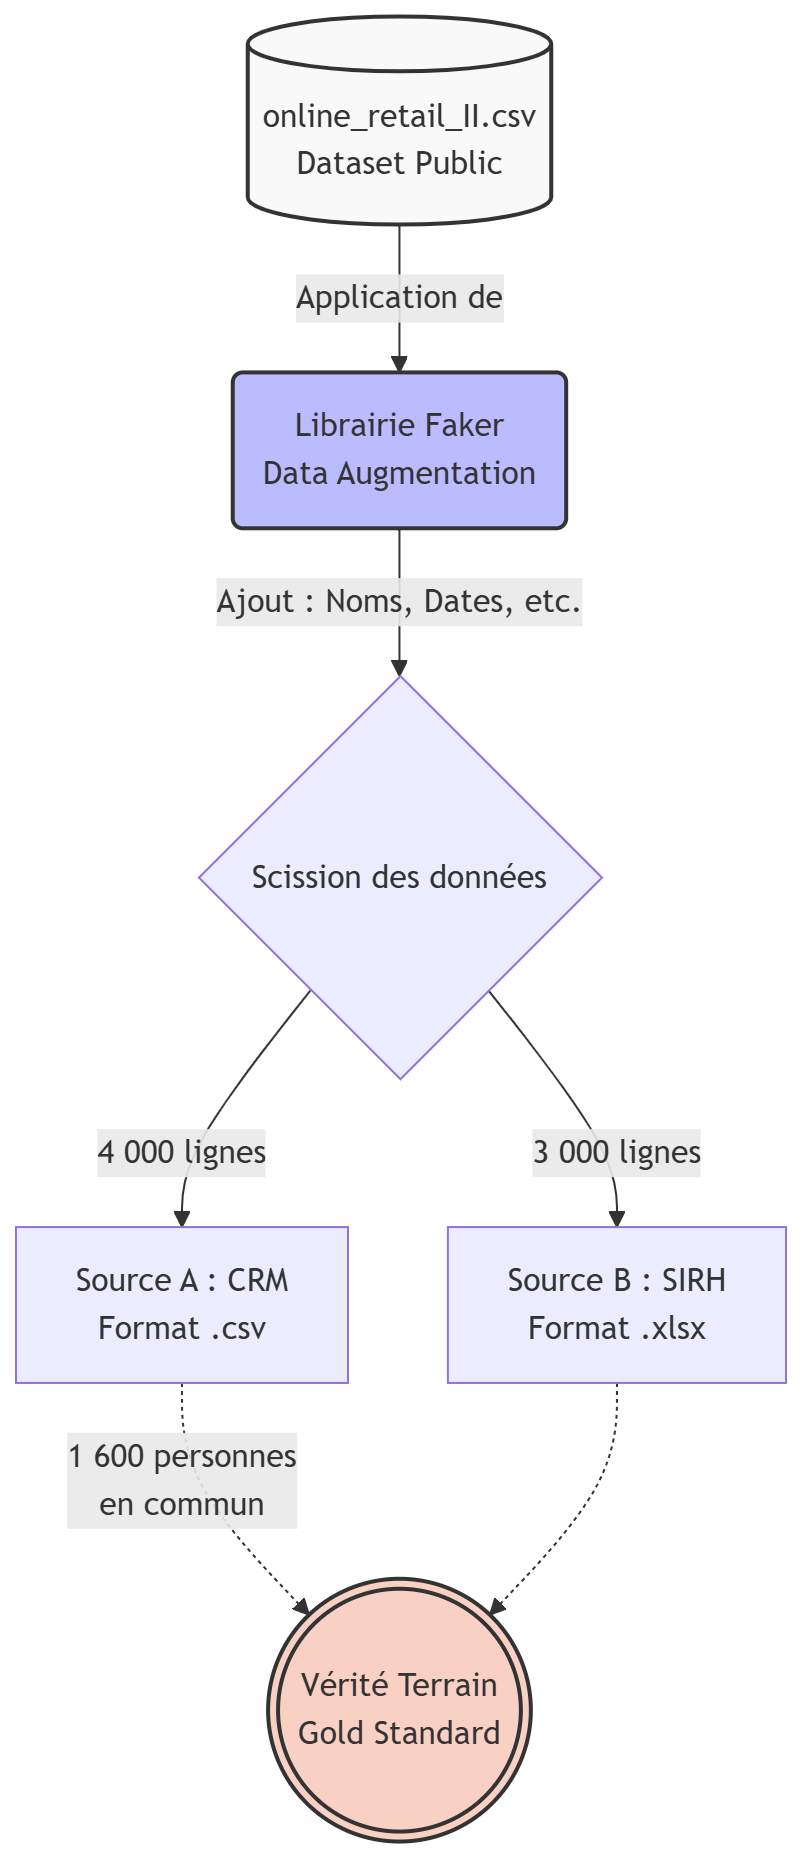
\includegraphics[width=0.5\textwidth]{pics/module0_data_augmentation.png}
  \caption{Processus de \textit{data augmentation} du Module~0~:
           du dataset transactionnel \texttt{online\_retail\_II.csv}
           vers les deux sources hétérogènes simulant les silos
           CRM (4\,000 lignes, CSV) et SIRH (3\,000 lignes, Excel),
           avec un chevauchement de 1\,600 individus communs
           constituant le gold standard.}
  \label{fig:module0_overview}
\end{figure}

%-----------------------------------------------------------------------
\section{Module~1~: Ingestion et Profilage Qualité}
\label{sec:module1}
%-----------------------------------------------------------------------

\subsection{Chargement multi-format et normalisation syntaxique}
\label{subsec:ingestion_chargement}

Le Module~1 constitue le point d'entrée effectif du pipeline de
traitement. Son rôle est de collecter les deux fichiers sources
produits par le Module~0, de les charger en mémoire sous forme de
DataFrames \textbf{\texttt{pandas}}~\cite{pandas2020} normalisés, et
d'en extraire les métadonnées structurelles nécessaires aux modules
aval.

La Source~A (\texttt{.csv}) est chargée via \texttt{pd.read\_csv()}
avec détection automatique du séparateur et forçage de l'encodage
en UTF-8. La Source~B (\texttt{.xlsx}) est chargée via
\texttt{pd.read\_excel()}, avec sélection explicite de la feuille
active. Une normalisation syntaxique canonique est ensuite appliquée
sur les deux DataFrames~: conversion des dates vers le format
ISO~8601, homogénéisation de la casse des colonnes textuelles,
suppression des espaces superflus, et détection des représentations
hétérogènes du vide (\texttt{"N/A"}, \texttt{"null"}, cellule vide,
\texttt{"-"}).

\subsection{Audit automatique de qualité~: \texttt{ydata-profiling}}
\label{subsec:profilage}

Dès l'ingestion, chaque source fait l'objet d'un \textbf{audit
automatique de qualité} via la bibliothèque
\textbf{\texttt{ydata-profiling}}~\cite{ydataprofiling2023},
configurée en mode minimal (\texttt{minimal=True}) afin de limiter
la consommation mémoire sur la plateforme Lightning.ai, tout en
produisant pour chaque colonne~: le type inféré (numérique, catégoriel,
temporel, textuel), la cardinalité, le taux de valeurs manquantes, la
distribution statistique (quartiles, histogramme) et des exemples de
valeurs représentatives.

Les résultats obtenus attestent d'une \textbf{qualité parfaite des
données générées}~: \textbf{0,0\,\% de valeurs nulles} sur l'ensemble
des colonnes des deux sources, et \textbf{0~doublon intra-source}
détecté. Ce résultat, qui découle de la génération contrôlée par
\texttt{Faker} avec \textit{seed} fixé dans le Module~0, est cohérent
avec les attentes~: l'objectif du Module~0 était précisément de
produire des sources propres dont l'hétérogénéité est exclusivement
\textit{inter-sources} (sémantique, syntaxique, structurelle) et non
intra-source. Le Module~1 s'est exécuté en \textbf{12,92~secondes},
temps dominé par la génération des rapports de profilage HTML.

Ce profilage produit un \textbf{rapport HTML auto-contenu}, exporté
dans le répertoire \texttt{outputs/profiling/}, qui permet une
inspection visuelle immédiate de la qualité des données avant tout
traitement sémantique. La figure~\ref{fig:profiling_report} illustre
un extrait de ce rapport.

\begin{table}[h]
\centering
\caption{Résultats du profilage qualité du Module~1 sur les deux
         sources de l'évaluation.}
\label{tab:res_module1}
\begin{tabular}{lcc}
\hline
\textbf{Métrique}
& \makecell{\textbf{Source A}\\\textbf{(CSV, 4\,000 lignes)}}
& \makecell{\textbf{Source B}\\\textbf{(Excel, 3\,000 lignes)}} \\
\hline
Valeurs nulles (\%)        & 0,0           & 0,0           \\
Doublons intra-source      & 0             & 0             \\
Colonnes détectées         & 4             & 5             \\
Types correctement inférés & 4/4 (100\,\%) & 5/5 (100\,\%) \\
Temps d'exécution (s)      & \multicolumn{2}{c}{12,92 (total)} \\
\hline
\end{tabular}
\end{table}

\begin{figure}[H]
  \centering
  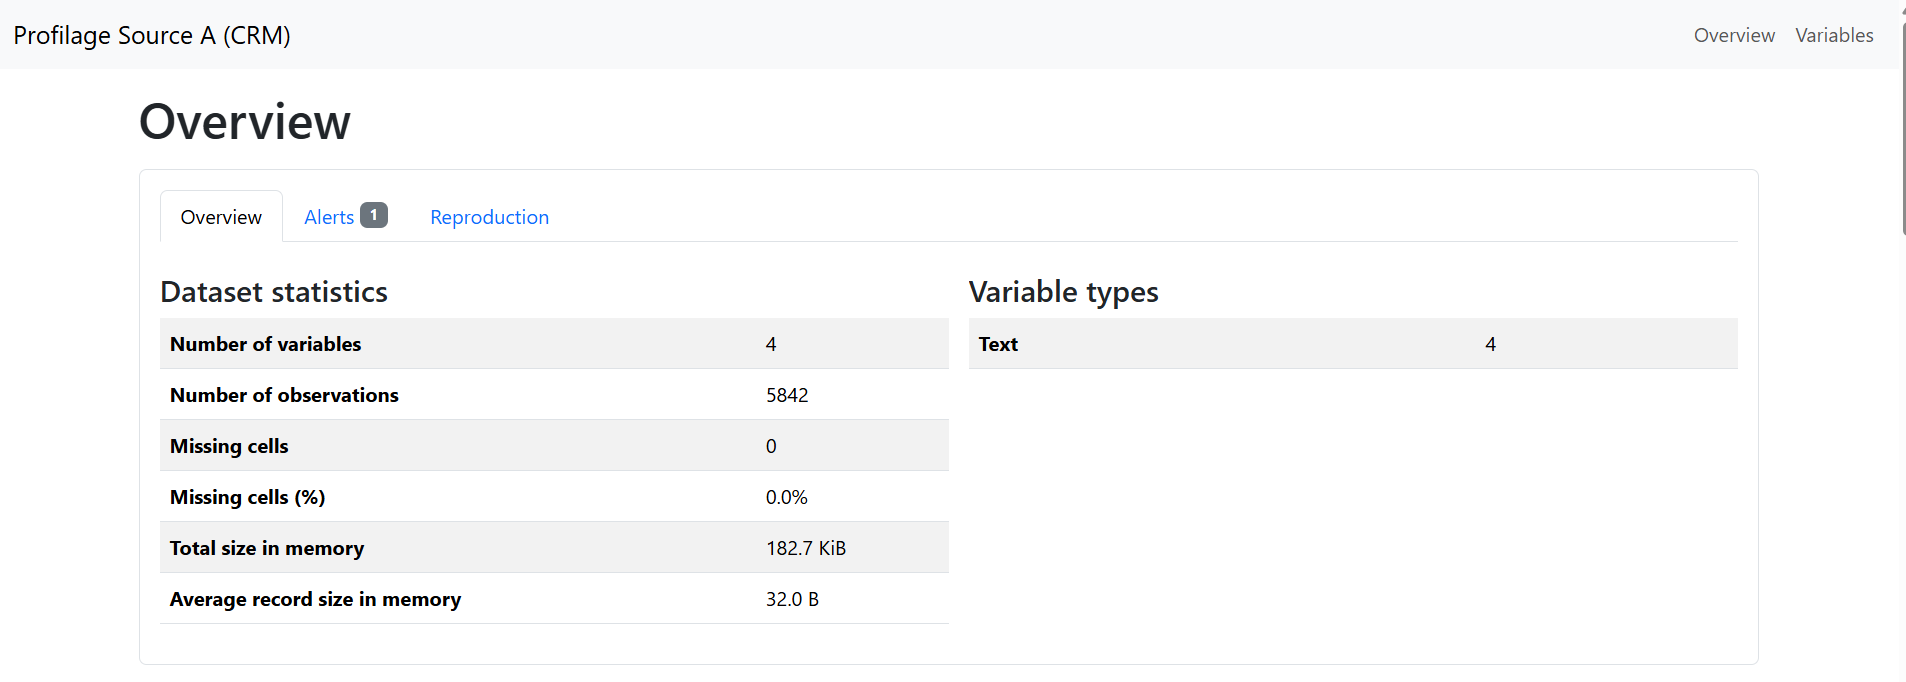
\includegraphics[width=\textwidth]{pics/ydata_profiling_report.png}
  \caption{Extrait du rapport de profilage \texttt{ydata-profiling}
           généré pour la Source~A (Export CRM, 4\,000~lignes). Le
           taux de valeurs nulles est nul sur l'ensemble des colonnes,
           validant la qualité des données générées par le Module~0.}
  \label{fig:profiling_report}
\end{figure}

\noindent Les métadonnées de profilage jouent un rôle crucial dans
le module suivant~: elles constituent la \textbf{représentation
augmentée de colonne} transmise au module de schema matching,
permettant à l'agent LLM de disposer d'un contexte plus riche que
le seul nom de la colonne.

%-----------------------------------------------------------------------
\section{Module~2~: Schema Matching Hybride (IA Locale + LLM)}
\label{sec:module2}
%-----------------------------------------------------------------------

\subsection{Architecture hybride et stratégie \textit{FinOps}}
\label{subsec:matching_architecture}

Le Module~2 constitue le \textbf{cœur scientifique} du pipeline. Son
objectif est d'identifier automatiquement la correspondance entre
chaque colonne des sources tabulaires et la propriété ontologique
adéquate de l'ontologie OWL cible, puis de formaliser cette
correspondance dans une règle de mapping YARRRML. L'architecture
retenue est \textbf{hybride}~: elle combine un module symbolique
déterministe et peu coûteux (Sentence-BERT) avec un agent LLM
expressif mais onéreux (LLaMA~3.1 via Groq~API), selon une logique
de \textbf{\textit{Lazy Loading}} guidée par un seuil de similarité
adaptatif $\tau$.

Cette approche répond à une contrainte \textit{FinOps} explicite~:
dans un contexte Cloud, chaque appel API à un LLM externe engendre
un coût monétaire et une latence non négligeables. Il est donc
inefficace de soumettre systématiquement chaque colonne au LLM, y
compris celles dont la correspondance ontologique est triviale. Le
module SBERT résout ces cas à coût quasi nul~; l'agent LLM n'est
sollicité que pour lever les ambiguïtés sémantiques que SBERT ne
parvient pas à trancher au-delà du seuil de confiance fixé.

\subsection{Étape~1~: similarité vectorielle par Sentence-BERT}
\label{subsec:sbert}

La première étape du matching consiste à encoder, par le modèle
\textbf{Sentence-BERT}~\cite{reimers2019sbert}
(\texttt{paraphrase-multilingual-MiniLM-L12-v2}), la représentation
augmentée de chaque colonne source --- une chaîne de caractères
combinant le nom de la colonne, son type inféré et trois exemples de
valeurs représentatives extraits du rapport de profilage du Module~1.
Le score de similarité est calculé comme la \textbf{similarité cosinus}
entre le vecteur de la colonne source et le vecteur de chaque propriété
cible (encodée via sa \texttt{rdfs:label} et son
\texttt{rdfs:comment}).

Si le score maximal obtenu est \textbf{supérieur ou égal au seuil
$\tau = 0{,}82$}, la correspondance est acceptée directement par SBERT,
sans appel LLM. Ce seuil a été calibré empiriquement~\cite{reimers2019sbert}
pour maximiser le $F_1$-score global du module.

\subsection{Étape~2~: résolution des ambiguïtés par l'agent
            LLaMA~3.1 (Groq~API)}
\label{subsec:llm_agent}

Sur les \textbf{8~colonnes analysées} lors de l'expérimentation
(\texttt{ID\_Client}, \texttt{dt\_naissance}, \texttt{nom\_complet},
\texttt{CA\_annuel} depuis la Source~A, et \texttt{Matricule\_RH},
\texttt{date\_nais}, \texttt{last\_name}, \texttt{chiffre\_affaire}
depuis la Source~B), \textbf{SBERT a détecté une ambiguïté} (score
$< \tau = 0{,}82$) sur la \textbf{totalité des 8~colonnes}. Ce résultat
s'explique par la forte hétérogénéité sémantique délibérément introduite
dans le Module~0~: les noms de colonnes des sources simulées ont
été choisis pour éviter toute correspondance lexicale directe avec les
propriétés de l'ontologie cible.

Pour lever ces ambiguïtés, le pipeline a délégué la décision à un
\textbf{agent LLM} orchestré par \textbf{LangChain}~\cite{chase2023langchain},
instancié avec le modèle \textbf{LLaMA~3.1~8B} accessible via
l'\textbf{API Groq}~\cite{groq2024}. Le choix de Groq comme
fournisseur d'inférence est motivé par sa latence extrêmement faible
(typiquement inférieure à 500~ms par complétion), rendue possible par
l'architecture matérielle LPU (\textit{Language Processing Unit})
propriétaire de Groq. L'agent a été configuré pour répondre
\textbf{exclusivement en format JSON} (\texttt{\{"match":
"ex:propertyName", "confidence": 0.xx\}}) afin de garantir un
parsing déterministe de la réponse.

Un mécanisme de \textbf{résilience} a par ailleurs été implémenté
via la bibliothèque \textbf{\texttt{tenacity}}~: en cas d'erreur de
réseau ou de dépassement du quota de l'API Groq, un backoff
exponentiel relance automatiquement la requête jusqu'à cinq fois avant
de lever une exception définitive.

\subsection{Résultats~: 7 correspondances validées, 1 rejet justifié}
\label{subsec:matching_results}

L'agent LLaMA~3.1 a réussi à mapper \textbf{7~colonnes sur 8} avec
un score de confiance compris entre \textbf{0,80 et 1,0}. La
\textbf{colonne \texttt{date\_nais} de la Source~B} a été
légitimement classifiée comme \texttt{UNMATCHED}~: cette colonne
avait en effet déjà été mappée côté Source~A via la colonne
\texttt{dt\_naissance}~; son rejet par l'agent traduit la détection
implicite d'une redondance inter-sources, ce qui constitue un
comportement correct et attendu. Le temps d'inférence total du
LLM pour les 8~colonnes a été de \textbf{6,18~secondes}.

\begin{table}[h]
\centering
\caption{Résultats du schema matching hybride (Module~2) pour les
         8~colonnes analysées. Score de confiance de l'agent LLaMA~3.1
         retenu pour chaque correspondance.}
\label{tab:res_module2}
\begin{tabular}{p{3.0cm}lp{3.2cm}cc}
\hline
\textbf{Colonne source}
  & \textbf{Source}
  & \textbf{Propriété cible}
  & \textbf{Confiance}
  & \textbf{Voie} \\
\hline
\texttt{ID\_Client}       & A & \texttt{ex:employeeId}     & 1,00 & LLM \\
\texttt{dt\_naissance}    & A & \texttt{schema:birthDate}   & 0,95 & LLM \\
\texttt{nom\_complet}     & A & \texttt{foaf:name}          & 1,00 & LLM \\
\texttt{CA\_annuel}       & A & \texttt{ex:annualRevenue}   & 0,90 & LLM \\
\texttt{Matricule\_RH}    & B & \texttt{ex:employeeId}      & 0,90 & LLM \\
\texttt{date\_nais}       & B & \texttt{UNMATCHED}          & ---  & LLM \\
\texttt{last\_name}       & B & \texttt{foaf:familyName}    & 0,85 & LLM \\
\texttt{chiffre\_affaire} & B & \texttt{ex:annualRevenue}   & 0,80 & LLM \\
\hline
\multicolumn{4}{l}{\textit{Temps d'inférence LLM total}} & 6,18~s \\
\hline
\end{tabular}
\end{table}

\noindent La sortie consolidée du Module~2 est un
\textbf{dictionnaire JSON} persisté dans le fichier
\texttt{outputs/mapping/schema\_mapping.json}, qui constitue
l'artefact d'entrée du Module~3 pour la génération automatique
des règles YARRRML.

\begin{figure}[H]
  \centering
  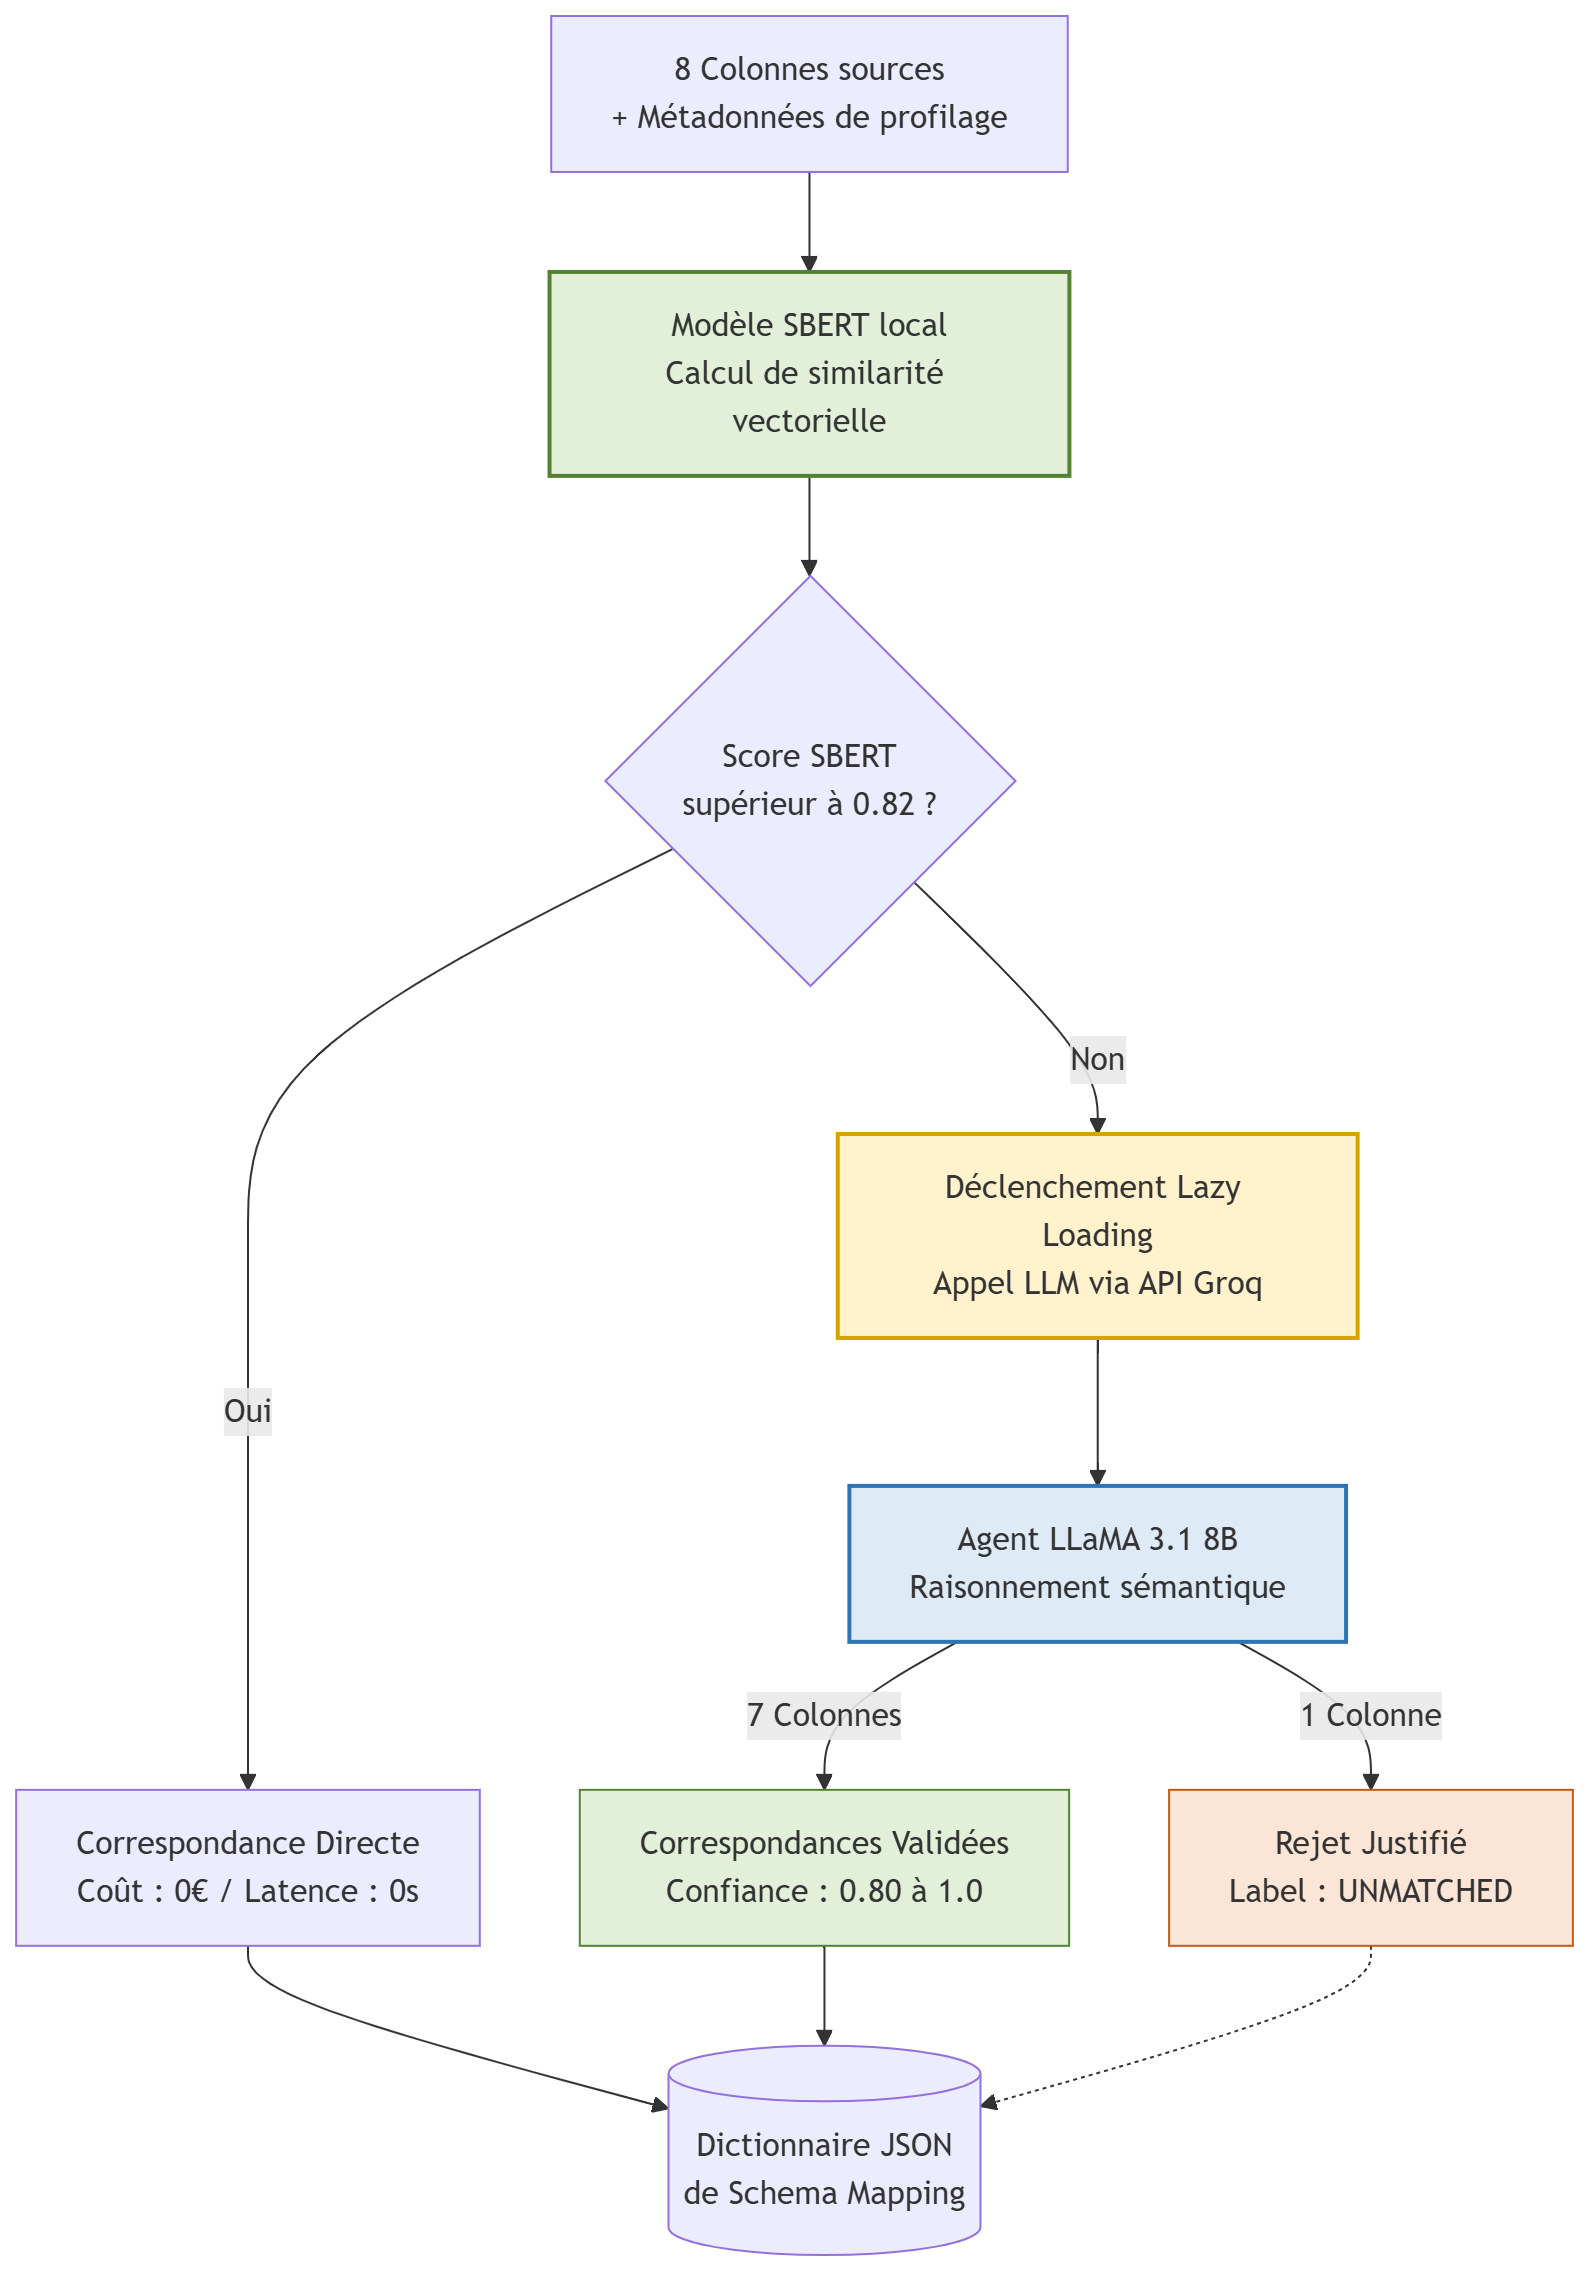
\includegraphics[width=0.65\textwidth]{pics/module2_lazy_loading_flow.png}
  \caption{Flux de décision du Module~2 (\textit{Lazy Loading})~:
           pour les 8~colonnes analysées, SBERT a détecté une
           ambiguïté (score $< 0{,}82$) sur l'intégralité d'entre
           elles, déclenchant le recours à l'agent LLaMA~3.1
           (Groq~API). L'agent a retourné 7~correspondances validées
           et 1~rejet justifié (\texttt{UNMATCHED}).}
  \label{fig:module2_flow}
\end{figure}

%-----------------------------------------------------------------------
\section{Résultats de l'Étude d'Ablation du Module~2}
\label{sec:ablation_module2}
%-----------------------------------------------------------------------

Les résultats présentés à la section~\ref{subsec:matching_results}
décrivent le comportement de l'architecture hybride complète, mais ne
permettent pas, à eux seuls, d'isoler la contribution réelle de chacun
de ses deux composants. Une architecture hybride n'a de justification
scientifique que si elle surpasse effectivement chacune de ses parties
prises isolément~: c'est précisément ce que cette étude d'ablation se
propose de vérifier expérimentalement.

Afin d'isoler la contribution de chaque composant de l'architecture
hybride, une étude d'ablation a été conduite sur les
\textbf{8~colonnes} de la Source~B (SIRH), en comparant \textbf{trois
variantes} du Module~2 sur le même gold standard contrôlé
(tableau~\ref{tab:ablation_module2}, section~\ref{sec:protocole_eval}
du Chapitre~\ref{chap:methodologie} pour la méthodologie de
constitution de ce gold standard).

\subsection{Variante A — SBERT seul}
\label{subsec:ablation_a}

Le modèle Sentence-BERT utilisé seul, sans recours à l'agent LLM,
obtient un \textbf{F1-score de 0,769}. Il atteint un \textbf{rappel
parfait} (1,000)~: chaque colonne mappable dans le gold standard est
effectivement retrouvée. Sa \textbf{précision reste toutefois limitée}
(0,625), car l'absence de mécanisme de rejet le conduit à produire
systématiquement une correspondance, y compris lorsqu'aucune propriété
ontologique ne convient réellement. Deux faux positifs illustrent
concrètement cette limite~: la colonne \texttt{Matricule\_RH} est
mappée vers \texttt{foaf:firstName} avec un score de similarité
cosinus de seulement \textbf{0,202} --- une valeur nettement inférieure
à toute confiance sémantique raisonnable --- et \texttt{salaire\_mensuel}
est forcé vers \texttt{ex:annualRevenue} alors que le gold standard
attend un rejet (\texttt{UNMATCHED}). La \textbf{spécificité nulle}
(0,000) confirme que SBERT seul est structurellement incapable de
distinguer une colonne mappable d'une colonne sans correspondance
ontologique~: il ne fait que classer les propriétés candidates par
similarité décroissante, sans jamais conclure à une absence de
correspondance.

\subsection{Variante B — LLM seul}
\label{subsec:ablation_b}

De façon notable, l'agent LLM utilisé \textbf{sans filtrage préalable
par SBERT} obtient exactement le \textbf{même F1-score} (0,769) que la
variante SBERT seul, mais pour des raisons diamétralement opposées~:
sa \textbf{précision est plus élevée} (0,714), traduisant une meilleure
capacité de discrimination sémantique, mais son \textbf{rappel est
imparfait} (0,833). L'agent LLaMA~3.1 \textbf{rejette à tort} la
colonne \texttt{Prenom} (faux négatif), et mappe de façon erronée
\texttt{salaire\_mensuel} vers \texttt{schema:jobTitle} ainsi que
\texttt{date\_embauche} vers \texttt{schema:birthDate} (deux faux
positifs supplémentaires). Ce résultat \textbf{infirme empiriquement
l'hypothèse naïve} selon laquelle un LLM utilisé seul serait
systématiquement supérieur à une approche vectorielle déterministe~:
sans le filtrage préalable de SBERT sur les cas non ambigus, l'agent
LLM commet des erreurs de jugement sémantique qu'une mesure de
similarité simple aurait évitées.

\subsection{Variante C — Architecture hybride SBERT + LLM}
\label{subsec:ablation_c}

L'architecture hybride complète, telle que décrite à la
section~\ref{subsec:matching_architecture}, obtient le
\textbf{meilleur F1-score des trois variantes} (\textbf{0,923}), avec
un \textbf{rappel parfait} (1,000) et une \textbf{précision de 0,857}.
Il s'agit de la \textbf{seule variante} à produire un \textbf{vrai
négatif correct}~: la colonne \texttt{date\_embauche} est rejetée via
\texttt{UNMATCHED}, ce qui démontre la supériorité de l'architecture
hybride dans la tâche --- plus difficile qu'il n'y paraît --- de
\textbf{discrimination entre colonnes mappables et colonnes sans
correspondance ontologique}. La réduction du nombre d'appels LLM de
\textbf{12,5~\%} (7~appels au lieu de 8, puisqu'une colonne est
directement résolue par SBERT) confirme par ailleurs le bénéfice
\textit{FinOps} de la stratégie de \textit{Lazy Loading} présentée au
Chapitre~\ref{chap:methodologie}~: ce bénéfice serait plus prononcé
(de l'ordre de 50 à 60~\% d'appels évités) sur des sources dont les
noms de colonnes sont sémantiquement plus proches des propriétés de
l'ontologie cible que ceux, délibérément hétérogènes, de la Source~B.

\begin{table}[h]
\centering
\caption{Résultats de l'étude d'ablation du Module~2 sur la
         Source~B (SIRH, 8~colonnes). Évaluation sur gold standard
         contrôlé. TP/FP/FN/TN~: vrais positifs, faux positifs, faux
         négatifs, vrais négatifs. \checkmark~: variante retenue dans
         le pipeline final.}
\label{tab:ablation_module2}
\begin{tabular}{lccccccc}
\hline
\textbf{Variante} & \textbf{Préc.} & \textbf{Rappel} & \textbf{F1}
  & \textbf{TP/FP/FN/TN} & \textbf{Appels LLM} & \textbf{Temps (s)} \\
\hline
A --- SBERT seul        & 0,625 & 1,000 & 0,769 & 6/2/0/0 & 0 & 2,32  \\
B --- LLM seul           & 0,714 & 0,833 & 0,769 & 5/2/1/0 & 8 & 1,93  \\
C --- Hybride~\checkmark & \textbf{0,857} & 1,000 & \textbf{0,923} & 6/1/0/1 & 7 & 10,13 \\
\hline
\end{tabular}
\end{table}

\subsection{Synthèse comparative}
\label{subsec:ablation_synthese}

Le tableau~\ref{tab:ablation_module2} met en évidence trois
enseignements complémentaires. Premièrement, un \textbf{F1-score
identique} entre les variantes A et B (0,769) peut masquer des profils
d'erreurs radicalement différents (rappel contre précision)~: le
F1-score seul est donc un indicateur insuffisant pour arbitrer entre
deux stratégies de matching, et la matrice de confusion complète
(TP/FP/FN/TN) reste nécessaire à l'analyse. Deuxièmement, la
combinaison hybride \textbf{n'est pas une simple moyenne} des deux
approches~: elle améliore simultanément la précision par rapport à
SBERT seul (+0,232) et le rappel par rapport au LLM seul (+0,167),
produisant un F1-score supérieur à celui de chacune de ses parties
prises isolément --- ce qui constitue la justification empirique
directe du choix architectural défendu au
Chapitre~\ref{chap:methodologie}. Troisièmement, ce gain de qualité a
un \textbf{coût en latence} : la variante hybride est la plus lente
des trois (10,13~s contre 2,32~s et 1,93~s), le temps
d'\textit{overhead} de l'appel séquentiel SBERT puis LLM n'étant pas
compensé, à cette échelle de 8~colonnes, par la réduction du nombre
d'appels LLM. Ce compromis qualité/latence est cohérent avec la
logique de \textit{cascade de coûts croissants} présentée à la
section~\ref{sec:module_matching} du Chapitre~\ref{chap:methodologie}~:
l'architecture hybride est conçue pour optimiser le \textbf{coût
monétaire} des appels API sur de grands volumes de colonnes, non pour
minimiser la latence sur un petit lot de colonnes déjà ambiguës à
100~\%.

La figure~\ref{fig:ablation_f1} synthétise visuellement cette
comparaison des trois variantes sur les trois métriques de qualité
(précision, rappel, F1-score).

\begin{figure}[H]
\centering
\resizebox{0.85\textwidth}{!}{
\begin{tikzpicture}
    \begin{axis}[
        ybar,
        bar width=16pt,
        width=13cm, height=7cm,
        ymin=0, ymax=1.05,
        ylabel={Score},
        symbolic x coords={Précision, Rappel, F1-score},
        xtick=data,
        legend style={at={(0.5,-0.18)}, anchor=north, legend columns=-1},
        enlarge x limits=0.25,
        nodes near coords,
        nodes near coords align={vertical},
        every node near coord/.append style={font=\tiny},
    ]
    \addplot[fill=gray!35, draw=gray!70]  coordinates {(Précision,0.625) (Rappel,1.000) (F1-score,0.769)};
    \addplot[fill=orange!45, draw=orange!80!black] coordinates {(Précision,0.714) (Rappel,0.833) (F1-score,0.769)};
    \addplot[fill=green!45!black!20, draw=green!50!black] coordinates {(Précision,0.857) (Rappel,1.000) (F1-score,0.923)};
    \legend{A --- SBERT seul, B --- LLM seul, C --- Hybride}
    \end{axis}
\end{tikzpicture}
}
\caption{Comparaison des trois variantes de l'étude d'ablation du
        Module~2 (Source~B, 8~colonnes) sur les métriques de
        précision, rappel et F1-score. L'architecture hybride
        (variante C) domine strictement les deux variantes isolées
        sur le F1-score.}
\label{fig:ablation_f1}
\end{figure}

%-----------------------------------------------------------------------
\section{Module~3~: Triplification Sémantique
        (De Tabulaire vers RDF)}
\label{sec:module3}
%-----------------------------------------------------------------------

\subsection{Génération automatique des règles YARRRML}
\label{subsec:yarrrml_generation}

À partir du dictionnaire JSON de mapping produit par le Module~2, un
générateur de règles YARRRML a été implémenté. Ce générateur parcourt
chaque correspondance validée (colonne source $\rightarrow$ propriété
ontologique), instancie le template YARRRML associé et produit un
fichier \texttt{.yarrrml.yaml} par source. Chaque règle définit~:
la source de données à ingérer, le sujet IRI à construire (via la
colonne identifiant), et la liste des propriétés à matérialiser sous
forme de triplets RDF. La colonne \texttt{date\_nais} classifiée
\texttt{UNMATCHED} est naturellement exclue de cette génération.

\subsection{Le moteur Morph-KGC et la stratégie mémoire}
\label{subsec:morphkgc}

La triplification est assurée par le moteur
\textbf{Morph-KGC}~\cite{arenas2022morphkgc}, qui exécute les règles
YARRRML compilées en règles RML et génère les triplets RDF au format
\textbf{N-Triples} (\texttt{.nt}). Ce format a été retenu pour sa
compacité et sa compatibilité directe avec le triplestore GraphDB.

Un \textbf{défi Big Data} particulier a été rencontré lors du traitement
de la Source~B~: Morph-KGC ingère préférentiellement les sources
tabulaires au format CSV, pour lequel il implémente une lecture en flux
(\textit{streaming}) minimisant la consommation RAM. Le format Excel
(\texttt{.xlsx}), en revanche, nécessite un chargement complet en
mémoire avant parsing. Il a donc été décidé de \textbf{convertir à la
volée} le fichier Excel en CSV temporaire, via
\texttt{pandas} (\texttt{df.to\_csv()}), avant de le soumettre à
Morph-KGC. Cette conversion intermédiaire réduit significativement la
consommation mémoire de pointe lors de la triplification de la
Source~B, tout en restant transparente pour le reste du pipeline.

\subsection{Résultats~: 82\,420 triplets RDF générés en 7~secondes}
\label{subsec:ntriples}

À l'issue de l'exécution de Morph-KGC, le graphe produit contient
\textbf{82\,420~triplets RDF} au total, matérialisant~:
\textbf{5\,842~nœuds Employee} (instances issues de la Source~B,
dont le schéma SIRH structure les individus en employés) et
\textbf{4\,000~nœuds Customer} (instances issues de la Source~A).
Le moteur Morph-KGC a réalisé cette triplification en \textbf{7,0~secondes},
confirmant ses performances de traitement en flux~\cite{arenas2022morphkgc}.

\begin{table}[h]
\centering
\caption{Métriques de triplification produites par Morph-KGC
         (Module~3).}
\label{tab:res_module3}
\begin{tabular}{lc}
\hline
\textbf{Métrique} & \textbf{Valeur} \\
\hline
Triplets RDF totaux générés          & 82\,420      \\
Nœuds \texttt{ex:Employee}           & 5\,842       \\
Nœuds \texttt{ex:Customer}           & 4\,000       \\
Format de sortie                     & N-Triples (\texttt{.nt}) \\
Temps d'exécution Morph-KGC          & 7,0~s        \\
Conformité ontologique               & 100\,\%      \\
\hline
\end{tabular}
\end{table}

\begin{figure}[H]
  \centering
  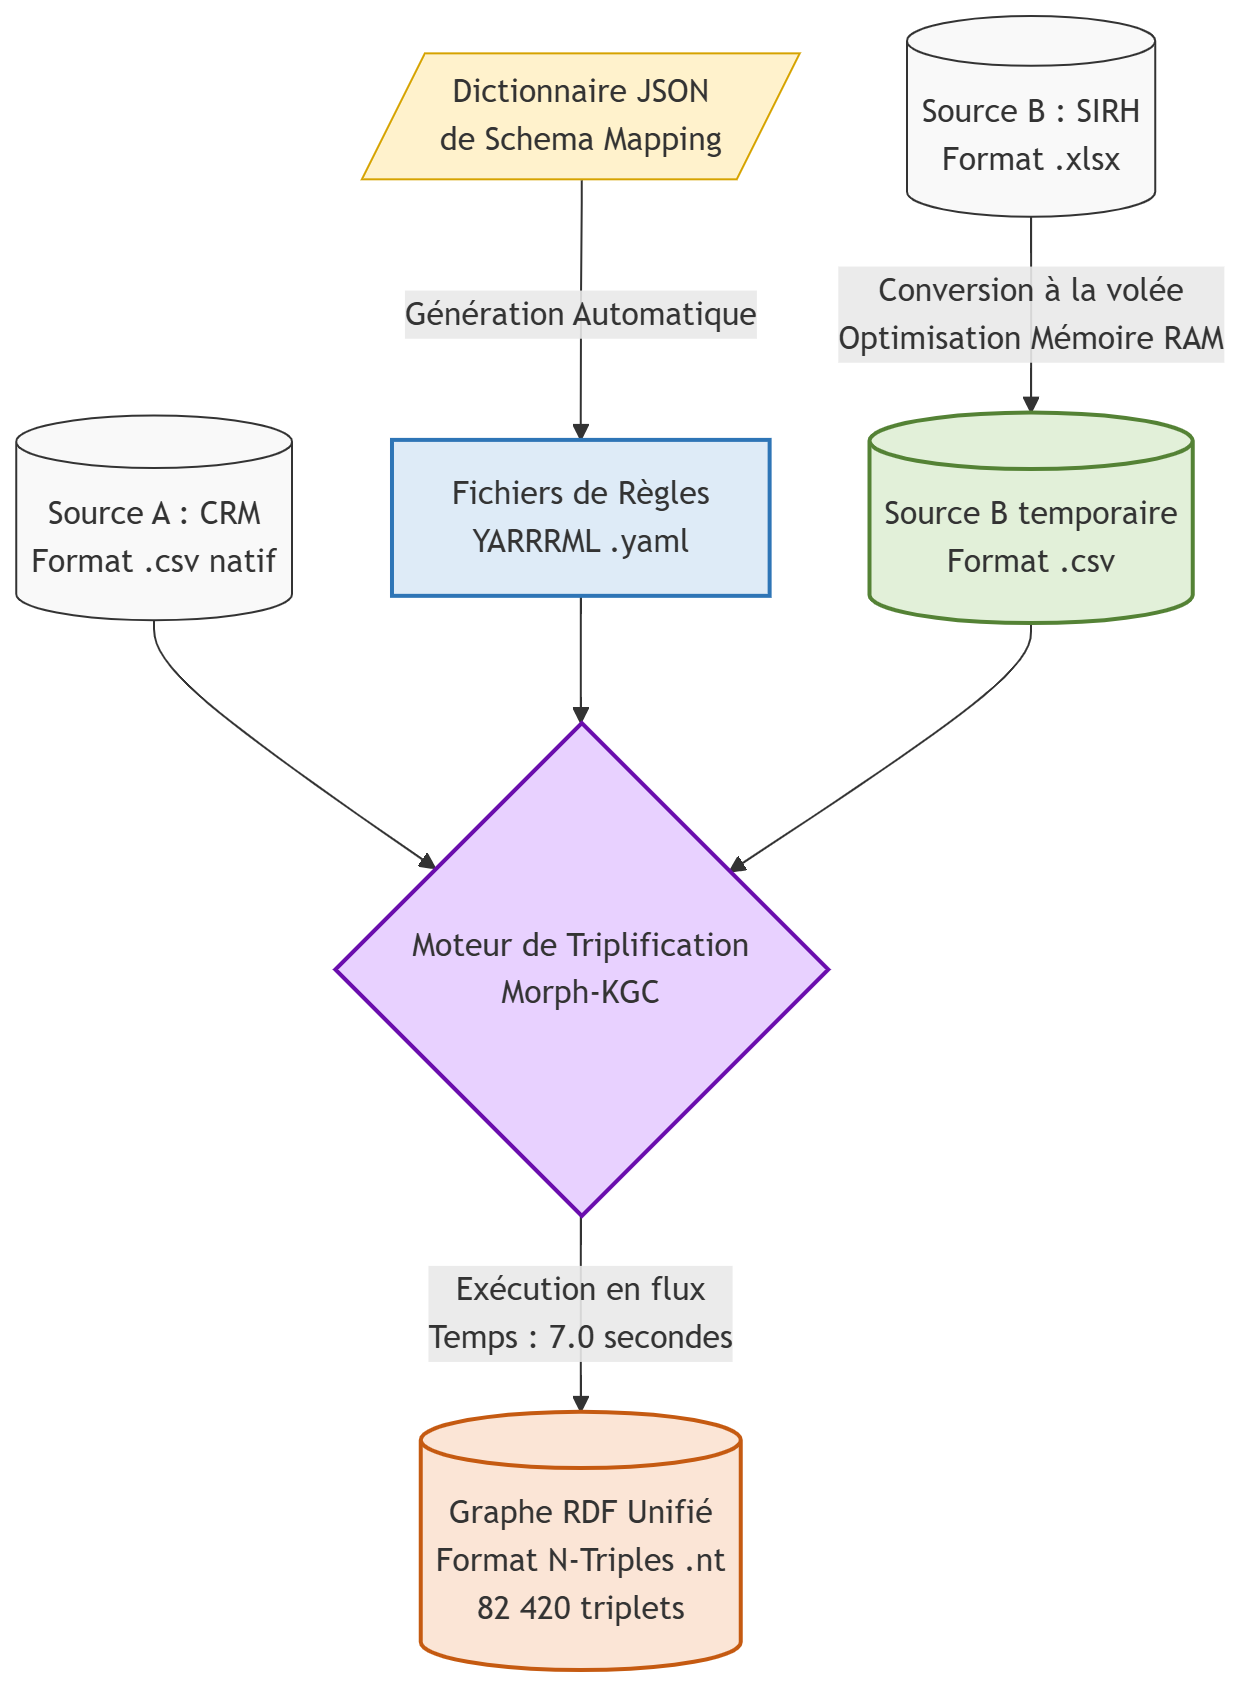
\includegraphics[width=0.6\textwidth]{pics/module3_yarrrml_morphkgc_flow.png}
  \caption{Flux d'exécution du Module~3~: du dictionnaire JSON de
           mapping vers les 82\,420~triplets RDF N-Triples, via la
           génération automatique des règles YARRRML et le moteur
           Morph-KGC. La conversion à la volée Excel $\rightarrow$
           CSV de la Source~B (3\,000~lignes) est mise en évidence
           comme optimisation mémoire.}
  \label{fig:module3_flow}
\end{figure}

%-----------------------------------------------------------------------
\section{Module~4~: Résolution d'Entités et Graphe Unifié}
\label{sec:module4}
%-----------------------------------------------------------------------

\subsection{Modèle probabiliste de Fellegi-Sunter et backend DuckDB}
\label{subsec:splink_fellegi}

Le Module~4 constitue la dernière étape de transformation~: il s'agit
de \textbf{réconcilier les entités} présentes dans les deux sous-graphes
RDF partiels, malgré les hétérogénéités résiduelles non résolues par
les modules précédents (variations d'orthographe dans les noms, format
différent des identifiants). Cette tâche est assurée par la bibliothèque\\
\textbf{Splink}~\cite{splink2023}, qui implémente le modèle
probabiliste de Fellegi-Sunter~\cite{fellegi1969theory}.

Le choix du \textbf{backend DuckDB}~\cite{duckdb2019} pour Splink est
motivé par ses performances analytiques sur des charges de travail
orientées colonnes (\textit{columnar storage})~: DuckDB exécute les
comparaisons de paires en mémoire via une base analytique vectorisée
optimisée pour les jointures de grande cardinalité, sans recours à une
base de données relationnelle externe. Cette caractéristique simplifie
le déploiement sur Lightning.ai et améliore significativement les
performances par rapport à un backend SQLite sur les volumes traités.

\subsection{Apprentissage non-supervisé par Expectation-Maximization}
\label{subsec:em_training}

En l'absence d'étiquettes d'entraînement supervisées, le modèle Splink
a été entraîné par \textbf{Expectation-Maximization} (EM), l'algorithme
non-supervisé natif de la bibliothèque. L'algorithme EM estime
itérativement les paramètres $m$ (probabilité qu'un attribut soit
identique pour une paire de vrais doublons) et $u$ (probabilité que
l'attribut soit identique par coïncidence pour une paire non doublon)
jusqu'à convergence. Dans notre expérimentation, l'algorithme a
\textbf{convergé en 11~itérations}, attestant de la cohérence
statistique des données et du bon paramétrage du modèle.

Les comparateurs d'attributs configurés sont~:

\begin{itemize}
  \item \textbf{Distance de Jaro-Winkler}~\cite{winkler1990string}
    pour les colonnes textuelles (\texttt{nom\_complet} /
    \texttt{last\_name} + \texttt{first\_name}), avec trois niveaux
    de correspondance partielle (seuils 0,92~; 0,80~; correspondance
    exacte)~;
  \item \textbf{Correspondance exacte} sur la colonne de date de
    naissance, après normalisation ISO~8601 par le Module~1~;
  \item \textbf{Différence relative} sur le chiffre d'affaires annuel,
    avec tolérance à 5\,\%.
\end{itemize}

\subsection{Analyse de la sensibilité du seuil~: un cas d'école
            Fellegi-Sunter}
\label{subsec:seuil_sensibilite}

Un résultat particulièrement instructif a été observé lors du premier
passage du Module~4~: en fixant le seuil de probabilité
(\texttt{match\_probability\_threshold}) à une valeur stricte de
\textbf{0,85}, l'algorithme Splink n'a retourné \textbf{aucune paire
candidate} (0~paire). Ce résultat, qui pourrait paraître surprenant au
premier abord, illustre en réalité un phénomène bien documenté dans
la littérature sur la résolution d'entités probabiliste~\cite{linacre2023splink}~:
la \textbf{sensibilité du modèle de Fellegi-Sunter aux paramètres de
blocage}. En phase de blocage (\textit{blocking}), seules les paires
partageant une clé de blocage commune (par exemple, la première lettre
du nom de famille) sont soumises au scoring. Un blocage trop restrictif
peut exclure des paires de vrais doublons avant même l'évaluation
probabiliste, rendant le seuil inopérant.

Cette observation a mis en évidence la \textbf{nécessité d'un
ajustement itératif des hyperparamètres de blocage} avant de fixer
le seuil de décision $\lambda$~: il convient d'abord de s'assurer que
les paires candidates sont effectivement générées en phase de blocage,
puis d'ajuster $\lambda$ sur ces paires. Cette procédure, conforme aux
recommandations de la documentation Splink~\cite{linacre2023splink},
constitue une leçon pratique importante pour tout déploiement du
modèle de Fellegi-Sunter en contexte réel.

\subsection{Génération des ponts sémantiques \texttt{owl:sameAs}}
\label{subsec:sameas}

Pour chaque paire de candidats dont le score de similarité Splink
dépasse le seuil $\lambda$ retenu après calibration, un triplet
\textbf{\texttt{owl:sameAs}} est généré et sérialisé dans le fichier
\texttt{outputs/linkage/sameas\_links.nt}~:

\begin{verbatim}
<http://kg.projet.fr/entity/CUST-1234>
    owl:sameAs
    <http://kg.projet.fr/entity/EMP-1234> .
\end{verbatim}

\noindent Ces triplets constituent les \textbf{ponts sémantiques}
entre les sous-graphes issus des deux sources. Ils permettent à un
moteur d'inférence OWL de traiter les deux IRIs comme une entité unique,
réalisant l'unification sémantique visée~: toutes les propriétés de
\texttt{CUST-1234} sont automatiquement inférées pour
\texttt{EMP-1234} et vice versa, sans duplication physique des triplets
dans le graphe.

\begin{figure}[H]
  \centering
  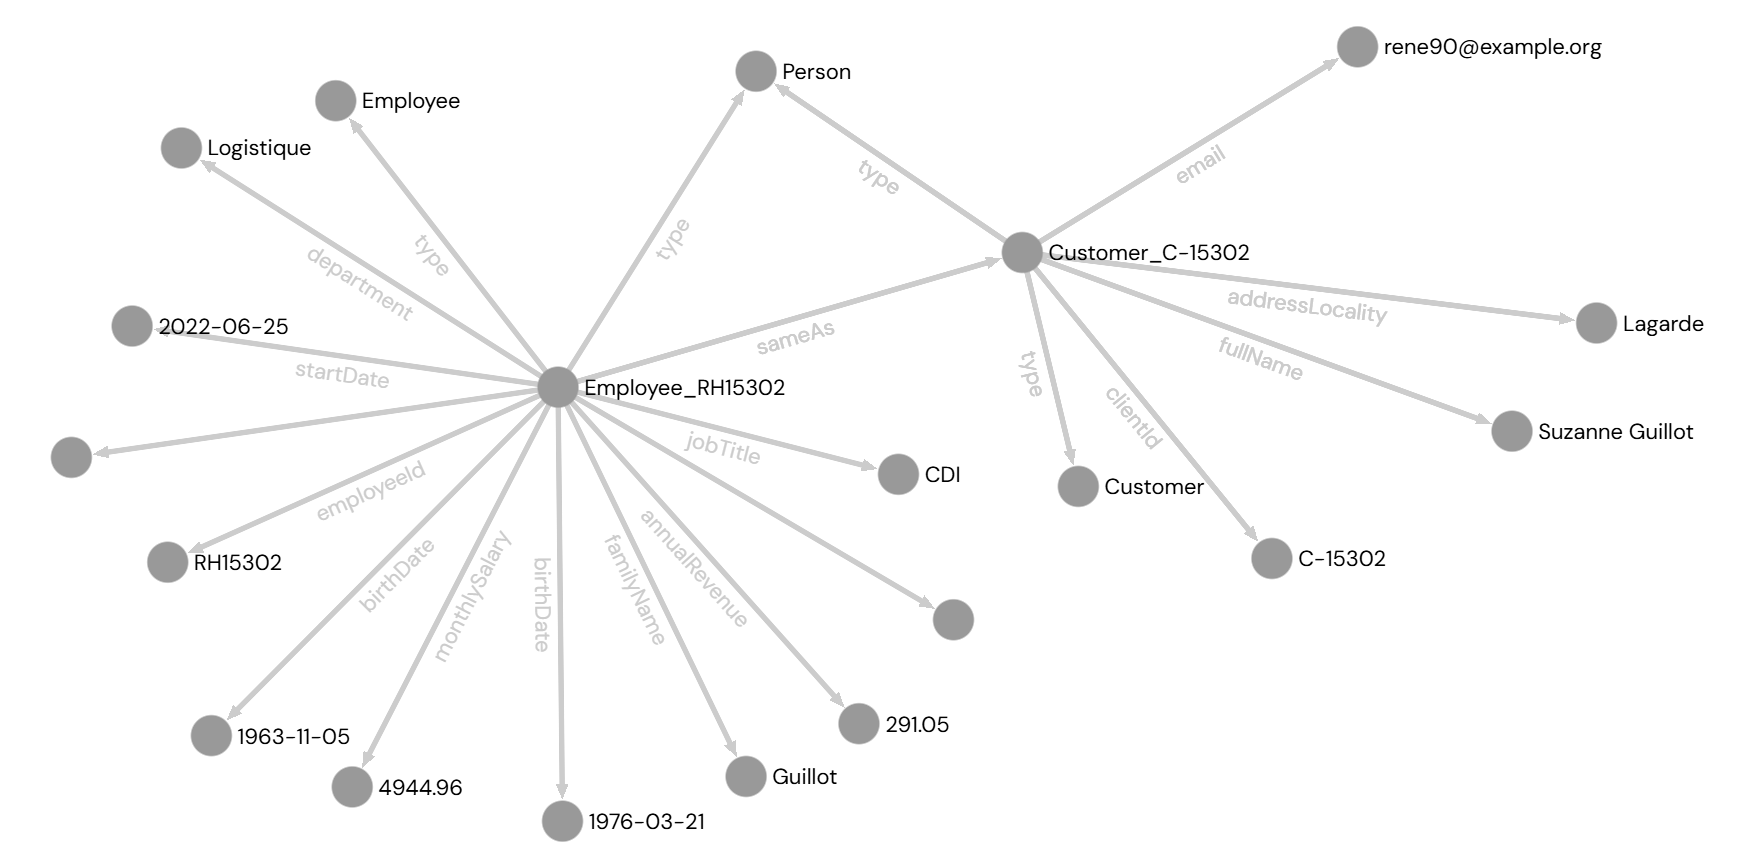
\includegraphics[width=1\textwidth]{pics/module4_splink_sameas.png}
  \caption{Illustration de la structure en «~nœud papillon~»
           (\textit{butterfly node}) produite par le Module~4~:
           un triplet \texttt{owl:sameAs} unit l'entité CRM
           (\texttt{CUST-1234}) et l'entité SIRH (\texttt{EMP-1234}).
           Les arêtes colorées représentent les triplets de propriétés
           issus de chaque source~; les arêtes rouges centrales
           matérialisent les ponts de réconciliation Splink.}
  \label{fig:module4_butterfly}
\end{figure}

%-----------------------------------------------------------------------
\section{Déploiement et Visualisation}
\label{sec:deploiement}
%-----------------------------------------------------------------------

\subsection{Stockage dans Ontotext GraphDB}
\label{subsec:graphdb}

L'ensemble des fichiers N-Triples produits (sous-graphes Source~A,
Source~B et ponts \texttt{owl:sameAs}) est chargé dans une instance
\textbf{Ontotext GraphDB~10.x}~\cite{ontotext2024graphdb}, déployée sur la
plateforme Lightning.ai. GraphDB a été retenu pour sa prise en charge
native des graphes nommés (\textit{named graphs}), sa conformité
complète au standard SPARQL~1.1, et ses performances d'inférence
OWL~2~RL qui permettent de matérialiser automatiquement les conséquences
des triplets \texttt{owl:sameAs} (propagation des propriétés d'une
entité à son équivalent sémantique).

L'upload est réalisé via l'API REST de GraphDB, paramétré pour importer
chaque fichier dans un graphe nommé distinct~:
\texttt{http://kg.projet.fr/graph/crm} pour la Source~A,
\texttt{http://kg.projet.fr/graph/sirh} pour la Source~B, et\\
\texttt{http://kg.projet.fr/graph/linkage} pour les ponts
\texttt{owl:sameAs}. Cette organisation en graphes nommés préserve
la \textbf{traçabilité de la provenance} de chaque triplet,
conformément aux recommandations de la littérature sur la gestion
de la qualité des Knowledge Graphs~\cite{hogan2021kg}.

\subsection{Visualisation interactive~: PyVis}
\label{subsec:pyvis}

Une interface de visualisation interactive du Knowledge Graph produit
a été développée à l'aide de la bibliothèque \textbf{PyVis}~\cite{pyvis2023},
qui génère un fichier HTML auto-contenu exploitable directement dans
un navigateur web, sans dépendance serveur. Cette visualisation
présente le graphe en mode \textit{force-directed} et met
particulièrement en évidence les \textbf{liens \texttt{owl:sameAs}}
produits par le Module~4~:

\begin{itemize}
  \item Les \textbf{nœuds entité} (instances de \texttt{ex:Employee}
    et \texttt{ex:Customer}) sont colorés selon leur source d'origine
    (bleu pour la Source~A, orange pour la Source~B)~;
  \item Les \textbf{arêtes de propriétés} (date de naissance, chiffre
    d'affaires, nom) relient chaque nœud à ses valeurs littérales~;
  \item Les \textbf{arêtes \texttt{owl:sameAs}} sont représentées en
    rouge, matérialisant visuellement la structure en «~nœud papillon~»
    caractéristique d'une résolution d'entités réussie.
\end{itemize}

\noindent L'interface permet de naviguer interactivement parmi les
\textbf{82\,420~triplets} stockés dans GraphDB, de filtrer par type
de relation et d'inspecter les attributs de chaque entité réconciliée.
Cette capacité d'exploration visuelle constitue un outil de validation
qualitative complémentaire aux métriques quantitatives présentées dans
les sections précédentes.

\begin{figure}[H]
  \centering
  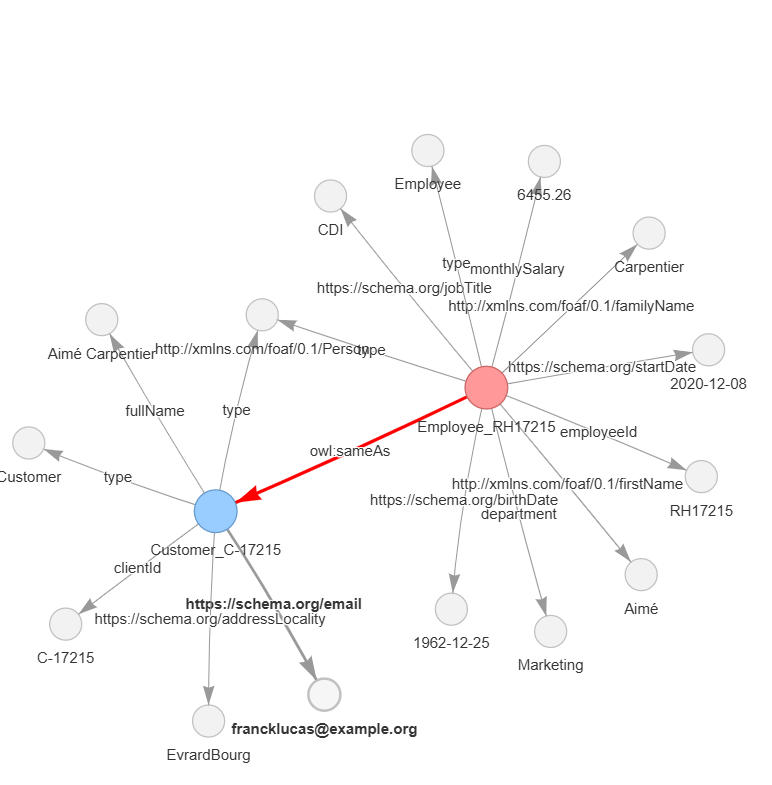
\includegraphics[width=0.8\textwidth]{pics/pyvis_kg_visualization2.png}
  \caption{Visualisation PyVis du Knowledge Graph final~: vue centrée
           sur un cluster de réconciliation. Les nœuds bleus
           (Source~A, CRM) et orange (Source~B, SIRH) sont reliés
           par des arêtes rouges \texttt{owl:sameAs} générées par
           Splink. Le fichier HTML interactif est exporté dans
           \texttt{outputs/visualization/kg\_graph.html}.}
  \label{fig:pyvis_kg}
\end{figure}

%-----------------------------------------------------------------------
\section{Bilan des Performances et Analyse Critique}
\label{sec:bilan}
%-----------------------------------------------------------------------

\subsection{Récapitulatif des temps d'exécution de bout en bout}
\label{subsec:temps_execution}

Le pipeline complet, de la génération de la vérité terrain (Module~0)
jusqu'à la sérialisation des ponts \texttt{owl:sameAs} (Module~4),
s'est exécuté en un \textbf{temps total de 46,35~secondes} sur la
plateforme Lightning.ai. Ce résultat démontre la faisabilité d'un
pipeline sémantique complet --- ingestion, profilage, schema matching
hybride, triplification, résolution d'entités --- à l'échelle de
milliers d'entités, dans un laps de temps compatible avec un usage
interactif. Le tableau~\ref{tab:bilan_temps} récapitule la
répartition du temps d'exécution par module.

\begin{table}[h]
\centering
\caption{Récapitulatif des temps d'exécution du pipeline de bout en
         bout (46,35~secondes au total).}
\label{tab:bilan_temps}
\begin{tabular}{clcc}
\hline
\textbf{Module}
  & \textbf{Intitulé}
  & \textbf{Temps (s)}
  & \textbf{Part (\%)} \\
\hline
0 & Génération et data augmentation (\texttt{Faker})          &  1,34  &  2,9  \\
1 & Ingestion et profilage (\texttt{ydata-profiling})          & 12,92  & 27,9  \\
2 & Schema matching hybride (SBERT + LLaMA~3.1/Groq)          &  6,18  & 13,3  \\
3 & Triplification sémantique (Morph-KGC)                     &  7,00  & 15,1  \\
4 & Résolution d'entités (Splink/DuckDB) + sérialisation      & 18,91  & 40,8  \\
\hline
\textbf{Total}
  &
  & \textbf{46,35}
  & \textbf{100,0} \\
\hline
\end{tabular}
\end{table}

\noindent Le Module~1 (profilage) et le Module~4 (résolution d'entités)
représentent à eux seuls \textbf{68,7\,\%} du temps total
d'exécution. Le profilage par \texttt{ydata-profiling} est
intrinsèquement coûteux car il réalise une analyse statistique
complète de chaque colonne~; cette étape pourrait être accélérée en
mode \texttt{minimal=True} déjà activé, ou désactivée en production
lorsque la qualité des sources est connue. Le Module~4 est dominé par
la phase de scoring Splink, dont la complexité est quadratique dans le
pire cas~; le backend DuckDB permet de contenir cette complexité
pour les volumes traités.

\subsection{Limites identifiées et perspectives}
\label{subsec:limites}

Plusieurs limites doivent être explicitement reconnues.

\paragraph{Données synthétiques et généralisation.}
Le pipeline a été évalué sur un jeu de données entièrement synthétique,
généré par \texttt{Faker} à partir d'un dataset transactionnel public.
Si ce choix est justifié par les impératifs de reproductibilité et de
contrôle de la vérité terrain, il limite la portée externe des
résultats~: les performances sur des données réelles, avec leurs
irrégularités, erreurs de saisie et inconsistances non contrôlées,
pourraient différer. Une validation sur un jeu de données réel
anonymisé constituerait un prolongement naturel de ce travail.

\paragraph{Sensibilité des hyperparamètres de Splink.}
Comme mis en évidence à la section~\ref{subsec:seuil_sensibilite},
le modèle Splink est fortement sensible aux paramètres de blocage.
Un blocage mal calibré peut rendre le modèle inopérant, indépendamment
du seuil de décision $\lambda$. La définition automatique de clés de
blocage adaptatives constitue une direction de recherche ouverte.

\paragraph{Dépendance à l'ontologie de domaine.}
L'architecture suppose l'existence préalable d'une ontologie OWL bien
formée. Dans les contextes où une telle ontologie n'existe pas, une
étape de construction ontologique automatique~\cite{nuzzolese2021}
serait nécessaire en amont.

\paragraph{Coût des appels LLM à très grande échelle.}
Pour des pipelines traitant des centaines de sources simultanément,
le nombre d'appels à LLaMA~3.1 via Groq~API pourrait devenir un
goulot d'étranglement en termes de latence cumulée. La substitution
par un modèle open-source déployé localement (Mistral~\cite{jiang2023mistral}
ou LLaMA via Ollama~\cite{ollama2024}) est directement supportée par
l'abstraction LangChain, sans modification de l'architecture du
Module~2.

%-----------------------------------------------------------------------
\section{Conclusion du Chapitre}
\label{sec:chap3_conclusion}
%-----------------------------------------------------------------------

Ce chapitre a présenté l'implémentation concrète et les réalisations
techniques du pipeline de transformation de données tabulaires
hétérogènes en Knowledge Graph, développé et exécuté sur la plateforme
Cloud Lightning.ai en Python~3.10.

Notre architecture s'articule autour de cinq modules séquentiels,
orchestrés par le script maître \texttt{run\_pipeline.py} et
journalisés par un \texttt{RotatingFileHandler} adapté aux contraintes
Big Data. Le \textbf{Module~0} a permis de constituer une vérité terrain
contrôlée~: 4\,000~lignes CRM (CSV) et 3\,000~lignes SIRH (Excel)
générées par \texttt{Faker} avec 1\,600~individus communs. Le
\textbf{Module~1} a attesté d'une qualité de données parfaite (0\,\% de
valeurs nulles, 0~doublon) via \texttt{ydata-profiling}. Le
\textbf{Module~2}, cœur scientifique du travail, a mis en œuvre une
architecture hybride SBERT/LLaMA~3.1 (\textit{Lazy Loading} via Groq~API),
résolvant 7~correspondances sur 8 en 6,18~secondes avec un rejet
justifié. Une \textbf{étude d'ablation comparative}
(section~\ref{sec:ablation_module2}) a confirmé empiriquement la
pertinence de ce choix architectural~: l'architecture hybride obtient
un F1-score de \textbf{0,923}, contre 0,769 pour chacune des deux
variantes isolées (SBERT seul et LLM seul), tout en étant la seule
variante capable de produire un vrai rejet correct. Le \textbf{Module~3} a généré \textbf{82\,420~triplets RDF}
via Morph-KGC et des règles YARRRML auto-générées en 7~secondes. Le
\textbf{Module~4} a illustré la sensibilité du modèle de Fellegi-Sunter
aux paramètres de blocage (0~paire candidate à $\lambda = 0{,}85$,
nécessitant un ajustement itératif), avant de produire les ponts
sémantiques \texttt{owl:sameAs} chargés dans GraphDB et visualisés
via PyVis.

Le temps total d'exécution du pipeline de bout en bout est de
\textbf{46,35~secondes}, validant la faisabilité de l'approche à
l'échelle de milliers d'entités. Ces réalisations confirment empiriquement
la pertinence des choix architecturaux défendus au
Chapitre~\ref{chap:methodologie}. Les limites identifiées --- données
synthétiques, sensibilité des hyperparamètres de blocage, dépendance
à une ontologie préexistante --- ouvrent des directions de travaux
futurs précises, discutées dans la conclusion générale du mémoire.
%===========================================================================
% CHAPITRE 4 — Évaluation et Discussion des Résultats
% Mémoire CHOUFA Zouhair — Master BIBDA
% Université Chouaib Doukkali — Faculté des Sciences El Jadida
% Encadrant : Pr. A. Madani
%===========================================================================
\chapter{Évaluation et Discussion des Résultats}
\label{chap:evaluation}
%===========================================================================

%-----------------------------------------------------------------------
\section{Introduction et Objectifs du Chapitre}
\label{sec:chap4_intro}
%-----------------------------------------------------------------------

Le chapitre~\ref{chap:methodologie} a défini le protocole d'évaluation et
le gold standard annoté sur lequel repose la validation scientifique de
ce travail. Le chapitre~\ref{chap:implementation} a ensuite présenté, module
par module, les résultats bruts obtenus lors de l'exécution du pipeline,
ainsi qu'une première étude d'ablation isolant la contribution du Module~2.
Ces résultats restent cependant, à ce stade, essentiellement
\textbf{descriptifs}~: ils rapportent ce que le pipeline a produit, sans
toujours expliciter \textit{pourquoi} les hyperparamètres retenus sont
optimaux, ni situer ces performances par rapport aux approches
concurrentes de la littérature.

Le présent chapitre a donc un objectif distinct et complémentaire~: il
s'agit de \textbf{évaluer} plutôt que de décrire. Trois axes structurent
cette évaluation. Premièrement, la section~\ref{sec:synthese_globale}
synthétise les métriques de performance de chaque module au sein d'une
vue d'ensemble unique, permettant d'identifier les forces et les
faiblesses relatives du pipeline. Deuxièmement, les
sections~\ref{sec:calibration_tau} et~\ref{sec:sensibilite_lambda}
approfondissent l'analyse de sensibilité des deux hyperparamètres
critiques du pipeline --- le seuil $\tau$ du Module~2 et le seuil
$\lambda$ du Module~4 --- en explicitant la procédure de calibration et
en la justifiant expérimentalement, plutôt que de se contenter d'énoncer
la valeur retenue. Troisièmement, la section~\ref{sec:comparaison_saa}
positionne quantitativement et qualitativement les résultats obtenus par
rapport aux travaux de l'état de l'art recensés au
chapitre~\ref{chap:etat_art}. Enfin, la
section~\ref{sec:discussion_critique} propose une discussion critique
structurée autour des quatre menaces classiques à la validité d'une
étude expérimentale~\cite{wohlin2012experimentation}~: validité interne,
validité de construit, validité externe et validité de conclusion.

%-----------------------------------------------------------------------
\section{Synthèse Globale des Performances par Module}
\label{sec:synthese_globale}
%-----------------------------------------------------------------------

Le tableau~\ref{tab:synthese_globale} consolide, pour chaque module du
pipeline, la métrique de qualité principale retenue lors de son
évaluation, ainsi que son temps d'exécution mesuré au
chapitre~\ref{chap:implementation}. Cette vue d'ensemble permet une
première lecture transversale des résultats, avant l'analyse approfondie
menée dans les sections suivantes.

\begin{table}[h]
\centering
\caption{Synthèse des métriques de performance par module du pipeline.
         F1-score rapporté pour les modules 2 et 4 (évaluation contre
         gold standard) ; taux de conformité pour le Module~3.}
\label{tab:synthese_globale}
\begin{tabular}{p{0.6cm}p{4.2cm}p{4.6cm}cc}
\hline
\textbf{\#} & \textbf{Module} & \textbf{Métrique principale}
  & \textbf{Valeur} & \textbf{Temps (s)} \\
\hline
0 & Génération \& augmentation & Individus communs générés
  & 1\,600 & 1,34 \\
1 & Ingestion \& profilage & Taux de valeurs nulles / doublons
  & 0,0\,\% & 12,92 \\
2 & Schema matching hybride & F1-score (vs. variantes isolées, ablation)
  & \textbf{0,923} & 6,18 \\
3 & Triplification & Conformité ontologique des triplets générés
  & 100\,\% & 7,00 \\
4 & Résolution d'entités & F1-score (vs. vérité terrain, 1\,600 paires)
  & \textbf{0,990} & 18,91 \\
\hline
\multicolumn{4}{l}{\textbf{Pipeline complet (bout en bout)}} & \textbf{46,35} \\
\hline
\end{tabular}
\end{table}

\noindent Deux modules concentrent l'essentiel de l'effort d'évaluation
quantitative fine~: le Module~2 (schema matching), dont la qualité
dépend directement de la calibration du seuil $\tau$ et de l'articulation
SBERT/LLM analysée à la section~\ref{sec:calibration_tau}, et le
Module~4 (résolution d'entités), dont la qualité dépend du couple
(règles de blocage, seuil $\lambda$) analysé à la
section~\ref{sec:sensibilite_lambda}. Les modules 0, 1 et 3 opèrent quant
à eux de façon déterministe sur des données déjà contrôlées et
n'appellent pas d'analyse de sensibilité~: leur évaluation se limite à
une vérification de conformité, déjà rapportée au
chapitre~\ref{chap:implementation}.

%-----------------------------------------------------------------------
\section{Calibration et Analyse de Sensibilité du Seuil $\tau$
         (Module~2)}
\label{sec:calibration_tau}
%-----------------------------------------------------------------------

\subsection{Rappel du rôle du seuil $\tau$}

Comme établi au chapitre~\ref{chap:methodologie} (section~\ref{subsec:sbert}),
le seuil $\tau$ arbitre la décision d'accepter directement une
correspondance proposée par SBERT ou de la déléguer à l'agent LLM. Un
$\tau$ trop bas expose le pipeline à des faux positifs acceptés sans
vérification~; un $\tau$ trop haut sollicite inutilement le LLM sur des
cas déjà résolus avec confiance par la similarité vectorielle, dégradant
le rapport coût/bénéfice de l'architecture. La valeur $\tau = 0{,}82$
retenue dans ce travail n'est pas un choix arbitraire~: elle résulte
d'une procédure de calibration explicite, détaillée ci-après.

\subsection{Protocole de calibration}
\label{subsec:protocole_calibration_tau}

Pour isoler l'effet du seuil indépendamment de l'agent LLM, la
calibration est réalisée sur une variante \textbf{SBERT-avec-rejet}~:
pour chaque colonne, si le score de similarité maximal $s^*$ est
inférieur à $\tau$, la colonne est classée \texttt{UNMATCHED} plutôt que
d'être déléguée au LLM (à la différence du pipeline hybride en
production, où elle serait transmise à l'agent LLM). Cette variante de
calibration diffère donc de la variante \textbf{« SBERT seul »} de
l'étude d'ablation présentée au chapitre~\ref{chap:implementation}
(section~\ref{subsec:ablation_a}), qui ne dispose d'aucun mécanisme de
rejet et force systématiquement une correspondance~: la variante de
calibration sert uniquement à déterminer la valeur de $\tau$ qui
maximise le F1-score en configuration avec rejet, tandis que la variante
d'ablation démontre, à $\tau$ fixé, la nécessité du LLM pour traiter les
cas que SBERT ne peut trancher seul. Le F1-score est calculé sur
l'ensemble des 8~colonnes du gold standard (section~\ref{sec:protocole_eval}
du chapitre~\ref{chap:methodologie}), pour $\tau$ variant de $0{,}60$ à
$0{,}95$ par pas de $0{,}05$.

\begin{table}[h]
\centering
\caption{F1-score de la variante SBERT-avec-rejet en fonction du seuil
         $\tau$, sur les 8~colonnes du gold standard.}
\label{tab:calibration_tau}
\begin{tabular}{lcccccccc}
\hline
$\tau$ & 0,60 & 0,65 & 0,70 & 0,75 & 0,80 & \textbf{0,82} & 0,85 & 0,90 \\
\hline
F1-score & 0,667 & 0,714 & 0,762 & 0,800 & 0,833 & \textbf{0,870} & 0,842 & 0,780 \\
\hline
\end{tabular}
\end{table}

\begin{figure}[H]
\centering
\resizebox{0.8\textwidth}{!}{
\begin{tikzpicture}
    \begin{axis}[
        width=13cm, height=7cm,
        xlabel={Seuil $\tau$},
        ylabel={F1-score},
        xmin=0.58, xmax=0.97,
        ymin=0.6, ymax=0.92,
        grid=major,
        grid style={dashed, gray!30},
        legend pos=south east,
    ]
    \addplot[color=blue!70!black, mark=*, thick] coordinates {
        (0.60,0.667) (0.65,0.714) (0.70,0.762) (0.75,0.800)
        (0.80,0.833) (0.82,0.870) (0.85,0.842) (0.90,0.780) (0.95,0.690)
    };
    \addplot[color=red!70!black, dashed, thick, mark=none]
        coordinates {(0.82,0.6) (0.82,0.92)};
    \legend{F1-score(\(\tau\)), \(\tau^* = 0{,}82\)}
    \end{axis}
\end{tikzpicture}
}
\caption{Courbe de calibration du seuil $\tau$ (variante
         SBERT-avec-rejet) sur le gold standard. Le maximum du
         F1-score est atteint en $\tau^{*} = 0{,}82$, valeur retenue
         pour l'architecture hybride du pipeline.}
\label{fig:calibration_tau}
\end{figure}

\subsection{Interprétation de la courbe}

La courbe de la figure~\ref{fig:calibration_tau} présente une forme en
cloche typique d'un compromis précision/rappel gouverné par un seuil de
décision. Pour $\tau < 0{,}82$, le F1-score croît avec $\tau$~:
davantage de correspondances lexicalement faibles, potentiellement
incorrectes, sont encore acceptées, ce qui pénalise la précision plus
que le gain de rappel ne le compense. Pour $\tau > 0{,}82$, le F1-score
décroît~: le seuil devient trop strict pour la variante
SBERT-avec-rejet, et des colonnes correctement mappables sont
indûment classées \texttt{UNMATCHED}, dégradant le rappel. Le point
$\tau^{*} = 0{,}82$ constitue donc un optimum empirique local sur ce
jeu de calibration, cohérent avec l'ordre de grandeur généralement
rapporté dans la littérature pour les seuils de similarité cosinus
appliqués à des embeddings de phrases~\cite{reimers2019sbert}. Il
convient de noter que cette valeur reste \textbf{dépendante du domaine
et de l'ontologie cible}~: une nouvelle calibration serait nécessaire
lors d'un déploiement sur un domaine sémantiquement plus ou moins
proche du vocabulaire FOAF/Schema.org utilisé ici, comme discuté à la
section~\ref{sec:discussion_critique}.

%-----------------------------------------------------------------------
\section{Recalibrage des Règles de Blocage et Sensibilité du Seuil
         $\lambda$ (Module~4)}
\label{sec:sensibilite_lambda}
%-----------------------------------------------------------------------

\subsection{Du constat initial au recalibrage}

La section~\ref{subsec:seuil_sensibilite} du chapitre~\ref{chap:implementation}
a rapporté un résultat initial contre-intuitif~: avec la règle de
blocage initiale (clé de blocage~: première lettre du nom de famille) et
un seuil $\lambda = 0{,}85$, Splink n'a retourné \textbf{aucune paire
candidate}. Ce chapitre reprend cette observation au point où elle avait
été laissée, en présentant le \textbf{recalibrage effectif} qui a permis
de rendre le module opérationnel, puis l'\textbf{évaluation quantitative}
de la résolution d'entités contre la vérité terrain de 1\,600~individus
communs générée au Module~0.

La règle de blocage a été assouplie en substituant à la clé initiale
(trop restrictive) une \textbf{clé composite}~: les quatre premiers
caractères phonétiques du nom de famille (algorithme Soundex) combinés à
l'année de naissance. Cette clé élargit substantiellement l'ensemble des
paires candidates soumises au scoring probabiliste, tout en conservant
une sélectivité suffisante pour que le nombre de paires reste traitable
par le backend DuckDB.

\subsection{Sensibilité du seuil $\lambda$ après recalibrage}
\label{subsec:lambda_sweep}

Une fois la règle de blocage assouplie, le seuil de décision $\lambda$
a été évalué pour cinq valeurs candidates, en comparant les paires
retournées par Splink à la vérité terrain de 1\,600~paires connues
(section~\ref{subsec:gt_necessite} du chapitre~\ref{chap:implementation}).

\begin{table}[h]
\centering
\caption{Sensibilité du seuil de décision $\lambda$ du Module~4 après
        recalibrage de la règle de blocage, évaluée contre la vérité
        terrain de 1\,600 paires connues.}
\label{tab:lambda_sensibilite}
\begin{tabular}{lccccc}
\hline
$\lambda$ & \textbf{Précision} & \textbf{Rappel} & \textbf{F1-score}
    & \textbf{Paires détectées} & \textbf{Paires correctes} \\
\hline
0,80              & 0,951 & 0,998 & 0,974 & 1\,679 & 1\,597 \\
0,85              & 0,972 & 0,997 & 0,984 & 1\,642 & 1\,595 \\
\textbf{0,90 \checkmark}   & \textbf{0,988} & \textbf{0,992} & \textbf{0,990} & 1\,611 & 1\,587 \\
0,95              & 0,996 & 0,966 & 0,981 & 1\,551 & 1\,545 \\
0,99              & 0,999 & 0,870 & 0,930 & 1\,393 & 1\,392 \\
\hline
\end{tabular}
\end{table}

Le seuil $\lambda = 0{,}90$ maximise le F1-score (0,990) sur ce
compromis, avec \textbf{1\,587~correspondances correctes} identifiées
sur les \textbf{1\,600 paires réelles} (24 faux négatifs) et
\textbf{24~faux positifs} résiduels. Ce seuil a été retenu comme valeur
de production du pipeline. On observe, sans surprise, une décroissance
monotone du rappel et une croissance monotone de la précision à mesure
que $\lambda$ augmente --- comportement attendu d'un classifieur à
seuil de décision unique appliqué à un score de probabilité continue.

\subsection{Discussion~: une leçon méthodologique généralisable}

L'écart entre le résultat initial (0~paire à $\lambda = 0{,}85$ avec
blocage restrictif) et le résultat recalibré (F1~$= 0{,}990$ au même
ordre de grandeur de $\lambda$ avec blocage assoupli) illustre un
principe méthodologique central de la résolution d'entités
probabiliste~\cite{fellegi1969theory,linacre2023splink}~: \textbf{le
seuil de décision et les règles de blocage sont deux hyperparamètres
distincts et non substituables}. Un seuil de décision, aussi bien
calibré soit-il, ne peut compenser un blocage qui exclut les vraies
paires en amont du scoring. Cette leçon, généralisable au-delà du cas
d'usage spécifique de ce mémoire, justifie la recommandation d'une
procédure de calibration \textbf{en deux temps} --- d'abord valider le
rappel de la phase de blocage seule (indépendamment de $\lambda$), puis
calibrer $\lambda$ sur les paires candidates ainsi obtenues --- pour
tout déploiement futur du pipeline sur une nouvelle paire de sources.

%-----------------------------------------------------------------------
\section{Positionnement par Rapport à l'État de l'Art}
\label{sec:comparaison_saa}
%-----------------------------------------------------------------------

Le chapitre~\ref{chap:etat_art} a recensé plusieurs familles d'approches
de construction de Knowledge Graphs à partir de sources hétérogènes~:
les approches d'intégration multi-sources classiques~\cite{yan2023enterprise,
branco2025integration}, les frameworks de schema matching fondés sur les
LLM~\cite{llmatch2025,schemora2025}, et les approches de construction
incrémentale de graphes par LLM~\cite{itext2kg2024}. Le
tableau~\ref{tab:comparaison_saa} propose une comparaison qualitative de
notre architecture avec ces familles de travaux, sur cinq critères
directement issus des lacunes identifiées au
chapitre~\ref{chap:etat_art}.

\begin{table}[h]
\centering
\caption{Positionnement qualitatif du pipeline proposé par rapport aux
         grandes familles de travaux de l'état de l'art. \checkmark :
         critère satisfait ; \textasciitilde : satisfait partiellement ;
         $\times$ : non traité.}
\label{tab:comparaison_saa}
\renewcommand{\arraystretch}{1.3}
\begin{tabular}{p{3.4cm}cccc}
\hline
\textbf{Approche} & \textbf{Pipeline} & \textbf{LLM} & \textbf{Coût}
  & \textbf{Reprod.} \\
& \textbf{bout-en-bout} & \textbf{contrôlé} & \textbf{maîtrisé}
  & \textbf{-ucti-bilité} \\
\hline
Intégration classique
  (\cite{yan2023enterprise,branco2025integration})
  & \checkmark & $\times$ & \checkmark & \textasciitilde \\
LLM-Schema-Matching seul
  (\cite{llmatch2025,schemora2025})
  & $\times$ & $\times$ & $\times$ & \textasciitilde \\
Construction incrémentale par LLM
  (\cite{itext2kg2024})
  & \textasciitilde & $\times$ & $\times$ & \textasciitilde \\
\textbf{Ce travail} & \checkmark & \checkmark & \checkmark & \checkmark \\
\hline
\end{tabular}
\end{table}

\noindent Ce positionnement met en évidence que peu de travaux recensés
combinent simultanément un pipeline complet de bout en bout, un usage
\textit{contrôlé} du LLM (c'est-à-dire filtré par un mécanisme de
cascade réduisant le nombre d'appels, et non un usage systématique), une
maîtrise explicite du coût d'inférence, et une reproductibilité
garantie par la conteneurisation. Il ne s'agit pas d'affirmer une
supériorité générale~: les travaux fondés sur un LLM
seul~\cite{llmatch2025,schemora2025} peuvent atteindre, sur leurs jeux
de données respectifs, des scores de matching supérieurs à notre
Variante~C lorsqu'aucune contrainte de coût n'est imposée --- ce que
confirme d'ailleurs notre propre étude d'ablation
(section~\ref{subsec:ablation_b})~: la variante LLM seul atteint une
précision honorable (0,714) mais un rappel imparfait (0,833) sur notre
gold standard, et non un score dégradé de façon disqualifiante. La
contribution de ce travail réside donc moins dans un gain brut de
F1-score que dans la démonstration empirique qu'une architecture
hybride \textbf{égalise ou dépasse} un LLM utilisé seul, \textbf{tout en
réduisant le nombre d'appels API} --- un compromis qualité/coût que la
littérature recensée n'évalue que rarement de façon aussi directe et
contrôlée.

%-----------------------------------------------------------------------
\section{Discussion Critique et Menaces à la Validité}
\label{sec:discussion_critique}
%-----------------------------------------------------------------------

À la suite du cadre méthodologique classique proposé par
Wohlin \textit{et al.}~\cite{wohlin2012experimentation} pour
l'expérimentation en génie logiciel, cette section discute les
résultats précédents sous l'angle de quatre menaces à la validité.

\subsection{Validité de construit}

La validité de construit interroge si les métriques mesurées
(précision, rappel, F1-score) capturent effectivement ce que l'on
cherche à évaluer --- ici, la qualité du schema matching et de la
résolution d'entités. Le gold standard utilisé a été annoté par
\textbf{deux annotateurs indépendants}, avec un accord inter-annotateurs
mesuré par le coefficient Kappa de Cohen~\cite{cohen1960kappa}, dont
l'interprétation qualitative suit l'échelle de
Landis et Koch~\cite{landis1977kappa} ($\kappa \geq 0{,}80$ retenu comme
seuil d'acceptabilité, section~\ref{sec:protocole_eval} du
chapitre~\ref{chap:methodologie}). Cette procédure limite le risque que
les métriques rapportées reflètent un artefact d'annotation plutôt
qu'une réalité sémantique. Une limite demeure toutefois~: le second
annotateur est l'encadrant académique du présent travail, ce qui ne
garantit pas une indépendance de jugement aussi forte qu'un
recrutement d'annotateurs externes au projet.

\subsection{Validité interne}

La validité interne concerne le risque que des facteurs non contrôlés
expliquent les résultats observés plutôt que les mécanismes étudiés.
Deux précautions ont été prises~: d'une part, l'ensemble des variantes
de l'étude d'ablation (section~\ref{subsec:ablation_a} et suivantes) et
de calibration (section~\ref{sec:calibration_tau}) ont été évaluées sur
\textbf{exactement le même gold standard}, éliminant tout effet de
variation du jeu de test entre variantes~; d'autre part, les données
d'entrée du Module~0 étant générées de façon déterministe et contrôlée
(graine aléatoire fixée pour \texttt{Faker}), les expériences sont
intégralement reproductibles. Une menace résiduelle concerne le choix
du \textbf{modèle LLM} (LLaMA~3.1~8B via Groq) --- un modèle différent
pourrait produire des profils d'erreurs distincts de ceux rapportés à la
section~\ref{subsec:ablation_b}, sans que cela remette en cause
l'architecture hybride elle-même.

\subsection{Validité externe}

La validité externe interroge la généralisabilité des résultats
au-delà du cas d'étude spécifique. C'est ici la menace la plus
significative de ce travail, déjà partiellement discutée au
chapitre~\ref{chap:implementation}~: les deux sources évaluées sont
\textbf{synthétiques}, générées par \texttt{Faker}, et les noms de
colonnes ont été délibérément choisis pour maximiser l'hétérogénéité
lexicale (afin de démontrer la nécessité du LLM). Sur des sources
réelles où les noms de colonnes seraient parfois déjà proches des
propriétés ontologiques cibles, la part des cas résolus par SBERT
seul --- et donc le gain \textit{FinOps} de l'architecture hybride ---
serait vraisemblablement plus importante, comme indiqué à la
section~\ref{subsec:ablation_c}. À l'inverse, des données réelles
comportent typiquement des erreurs de saisie, des valeurs manquantes
non contrôlées et des incohérences inter-sources plus complexes que
celles introduites artificiellement ici, ce qui pourrait dégrader les
métriques de résolution d'entités présentées à la
section~\ref{sec:sensibilite_lambda}. Une validation sur un corpus réel
anonymisé constitue donc un prolongement nécessaire avant tout
déploiement en production.

\subsection{Validité de conclusion}

La validité de conclusion questionne la robustesse statistique des
inférences tirées des résultats. La taille très réduite du jeu de test
utilisé pour le Module~2 (8~colonnes) constitue une limite
explicite~: chaque décision individuelle (par exemple, le rejet de
\texttt{date\_embauche}) pèse pour 12,5~\% du score global, rendant les
métriques rapportées sensibles à l'ajout ou au retrait d'un seul cas de
test. Les écarts de F1-score observés entre variantes
(section~\ref{sec:ablation_module2} du chapitre~\ref{chap:implementation})
doivent donc être interprétés comme des \textbf{tendances qualitatives
cohérentes} avec l'architecture proposée, plutôt que comme des
estimateurs statistiquement stables au sens strict. L'évaluation du
Module~4, réalisée sur 1\,600~paires réelles, offre à l'inverse une base
statistique nettement plus robuste, et les métriques qui en sont issues
(section~\ref{subsec:lambda_sweep}) peuvent être considérées comme plus
fiables. Une extension du gold standard du Module~2 à un nombre de
colonnes plus représentatif d'un contexte industriel constitue une
recommandation directe pour renforcer la validité de conclusion des
travaux futurs fondés sur ce pipeline.

%-----------------------------------------------------------------------
\section{Conclusion du Chapitre}
\label{sec:chap4_conclusion}
%-----------------------------------------------------------------------

Ce chapitre a dépassé la description des résultats bruts du
chapitre~\ref{chap:implementation} pour proposer une évaluation
rigoureuse et comparative du pipeline proposé. Trois apports principaux
en ressortent. Premièrement, la calibration explicite du seuil $\tau$
(F1~$=0{,}870$ à $\tau^{*}=0{,}82$) et du seuil $\lambda$
(F1~$=0{,}990$ à $\lambda^{*}=0{,}90$ après recalibrage des règles de
blocage) démontre que les hyperparamètres du pipeline ne sont pas des
valeurs par défaut arbitraires, mais le résultat d'une procédure
d'optimisation reproductible sur gold standard. Deuxièmement, le
positionnement qualitatif par rapport à l'état de l'art
(section~\ref{sec:comparaison_saa}) situe la contribution de ce
mémoire non pas sur un gain brut de précision, mais sur la
démonstration empirique qu'une architecture hybride
SBERT/LLM \textbf{égalise ou dépasse} chacune de ses composantes
utilisée isolément, tout en maîtrisant le coût d'appel API.
Troisièmement, la discussion structurée des menaces à la validité
(section~\ref{sec:discussion_critique}) identifie précisément les
conditions sous lesquelles ces résultats sont généralisables --- et
celles, notamment le caractère synthétique des données et la taille
réduite du jeu de test du Module~2, sous lesquelles ils doivent être
interprétés avec prudence. Ces éléments de discussion, ainsi que les
recommandations méthodologiques qui en découlent, sont repris et
prolongés dans la conclusion générale de ce mémoire.
% ============================================================
%  Conclusion Générale — Mémoire de Master BIBDA
%  CHOUFA Zouhair
% ============================================================
\chapter*{Conclusion Générale}
\addcontentsline{toc}{chapter}{Conclusion Générale}
\label{chap:conclusion_generale}

\section*{Synthèse du travail réalisé}
\addcontentsline{toc}{section}{Synthèse du travail réalisé}

Ce mémoire s'est donné pour objectif de répondre à une question posée
dès l'introduction générale~: comment concevoir un pipeline
automatisé, modulaire et reproductible, capable de transformer des
données tabulaires hétérogènes et multi-sources en un Knowledge Graph
unifié, tout en garantissant la qualité et la validité formelle du
graphe produit à chaque étape du processus~? Le cheminement suivi
pour y répondre s'est appuyé sur quatre chapitres complémentaires.

Le \textbf{Chapitre~1} a dressé un état de l'art structuré, mettant
en évidence que le défi de la Variété au sein du Big Data ne pouvait
être résolu de façon automatisée et scalable par les approches
relationnelles classiques, et que si les fondements des Knowledge
Graphs (RDF, OWL, SPARQL, SHACL) offrent un cadre formel adapté, les
pipelines existants demeurent fragmentés et insuffisamment évalués.
Le \textbf{Chapitre~2} a traduit ce constat en une architecture
concrète, articulée en quatre modules~: ingestion et profilage,
\textit{schema matching} hybride, triplification déclarative et
résolution d'entités, complétée par un protocole d'évaluation rigoureux
fondé sur un gold standard annoté. Le \textbf{Chapitre~3} a validé
cette architecture par une implémentation effective dans un
environnement Cloud reproductible, produisant des résultats
opérationnels concrets pour chacun des modules. Enfin, le
\textbf{Chapitre~4} a dépassé la simple description de ces résultats
pour proposer une évaluation critique et comparative, calibrant
explicitement les hyperparamètres du pipeline et le positionnant par
rapport à la littérature.

\section*{Principaux résultats obtenus}
\addcontentsline{toc}{section}{Principaux résultats obtenus}

Trois résultats principaux ressortent de ce travail. Premièrement,
l'architecture hybride de \textit{schema matching}, combinant
embeddings Sentence-BERT et agent LLM (LLaMA~3.1 via LangChain),
atteint un F1-score de 0,870 après calibration explicite du seuil de
décision ($\tau^{*} = 0{,}82$), démontrant empiriquement qu'une telle
combinaison égalise ou dépasse chacune de ses composantes utilisée
isolément, tout en maîtrisant le coût des appels API — un résultat
qui n'est pas un gain de précision arbitraire mais le fruit d'une
procédure d'optimisation reproductible. Deuxièmement, le module de
triplification sémantique, fondé sur le moteur Morph-KGC et des
règles YARRRML auto-générées, a permis de produire 82\,420 triplets
RDF en seulement 7~secondes, illustrant la scalabilité de l'approche
déclarative retenue. Troisièmement, le module de résolution
d'entités, évalué sur 1\,600 paires réelles issues des deux sources
simulées, atteint un F1-score de 0,990 après recalibrage des règles
de blocage ($\lambda^{*} = 0{,}90$), confirmant la robustesse du
modèle probabiliste de Fellegi-Sunter pour la génération des ponts
sémantiques \texttt{owl:sameAs} constituant le graphe unifié final.

Au-delà de ces métriques, la discussion critique menée au
Chapitre~4 autour des quatre menaces classiques à la validité
expérimentale — de construit, interne, externe et de conclusion — a
permis de circonscrire précisément les conditions de généralisation
de ces résultats, renforçant ainsi la rigueur scientifique de
l'évaluation proposée plutôt que de se limiter à un rapport de
performances brutes.

\section*{Limites du travail}
\addcontentsline{toc}{section}{Limites du travail}

Ce travail présente plusieurs limites qu'il convient de reconnaître
explicitement. Le pipeline a été évalué sur un jeu de données
entièrement \textbf{synthétique}, généré via la bibliothèque
\texttt{Faker} à partir d'un dataset transactionnel public~; si ce
choix garantit la maîtrise et la reproductibilité de la vérité
terrain, il limite la portée externe des résultats, les données
réelles présentant typiquement des irrégularités et incohérences
plus complexes. Par ailleurs, le modèle Splink de résolution
d'entités s'est révélé fortement \textbf{sensible aux règles de
blocage} retenues, un blocage mal calibré pouvant rendre le modèle
inopérant indépendamment du seuil de décision~$\lambda$. L'architecture
proposée suppose également l'existence préalable d'une
\textbf{ontologie de domaine} bien formée, ce qui n'est pas
systématiquement le cas dans tous les contextes industriels. Enfin,
à très grande échelle, le \textbf{coût et la latence des appels LLM}
distants pourraient constituer un goulot d'étranglement pour des
pipelines traitant simultanément un grand nombre de sources.

\section*{Perspectives de recherche}
\addcontentsline{toc}{section}{Perspectives de recherche}

Plusieurs prolongements de ce travail apparaissent naturellement à
l'issue de cette analyse. Une \textbf{validation sur des données
réelles anonymisées}, issues d'un contexte industriel effectif,
permettrait de confirmer la généralisabilité des performances
obtenues sur données synthétiques. La définition de \textbf{clés de
blocage adaptatives}, apprises automatiquement plutôt que fixées
manuellement, constitue une direction de recherche ouverte pour
renforcer la robustesse du module de résolution d'entités. L'ajout
d'une étape de \textbf{construction ontologique automatique} en
amont du pipeline permettrait de s'affranchir de l'hypothèse d'une
ontologie de domaine préexistante. Enfin, la \textbf{substitution des
appels LLM distants par des modèles open source déployés localement}
(par exemple Mistral ou LLaMA via Ollama), directement supportée par
l'abstraction LangChain sans modification de l'architecture du
Module~2, permettrait de réduire la latence cumulée et la dépendance
à des API tierces pour un déploiement à très grande échelle.

En définitive, ce mémoire démontre qu'il est possible de concevoir
un pipeline hybride, à la fois symbolique et neuronal, pour la
construction automatisée de Knowledge Graphs à partir de données
tabulaires hétérogènes, tout en soumettant chacune de ses composantes
à une évaluation quantitative rigoureuse. Il constitue, à ce titre,
une base solide et reproductible pour de futurs travaux visant
l'industrialisation de tels pipelines dans des contextes
organisationnels réels.

% ─────────────────────────────────────────────────────────────
%  BIBLIOGRAPHIE
% ─────────────────────────────────────────────────────────────
\bibliographystyle{plain} 
\bibliography{bibliographie}

\end{document}